\documentclass[11pt]{article}
\usepackage[review]{acl}

\usepackage{times}
\usepackage{latexsym}
\usepackage[T1]{fontenc}
\usepackage[utf8]{inputenc}
\usepackage{microtype}

\usepackage{amsmath}
\usepackage{amssymb}
\usepackage{graphicx}
\usepackage{booktabs}
\usepackage{subcaption}
\usepackage{dblfloatfix}
\usepackage{placeins}
\usepackage{algorithm}
\usepackage{algpseudocode}
\usepackage{amsthm}
\newtheorem{theorem}{Theorem}
\newtheorem{proposition}[theorem]{Proposition}
\newtheorem{designprinciple}[theorem]{Design Principle}
\theoremstyle{definition}
\newtheorem{assumption}[theorem]{Assumption}

\title{Characterizing the Detectability Landscape of Iterative Model Collapse}

\author{Anonymous}

\begin{document}
\maketitle

\begin{abstract}
As machine-generated text proliferates online, language models increasingly risk training on their own output, creating a feedback loop driving iterative model collapse that erodes diversity and calibration across generations.
While collapse dynamics are increasingly understood, \emph{detecting} onset remains open: iterative training yields short, noisy time series ($T{<}15$) resisting early-warning diagnostics, collapse is a first-order transition precluding critical-slowing-down signals, and no prior work systematically compares detection methods on this problem.
We map the \emph{detectability landscape} (how detection varies across contamination levels, observation windows, and statistical methods) on five model families (345M--6.9B).
A steep onset emerges: permutation Granger testing finds zero significant canary$\to$downstream pairs through 45\% contamination, then jumps to reliable detection (6/8 pairs; 95\% CI $[0.25, 0.92]$) within two percentage points, defining blind, onset, and detection regimes.
Across five methods, null-control false-positive rates span 7\%--94\%, revealing that method choice alone determines whether collapse appears detectable.
Token entropy precedes diversity decline by ${\geq}1$ generation, enabling proof-of-concept intervention reducing peak perplexity by 64\%\footnote{Code and data are available at \url{https://anonymous.4open.science/r/distrib_canary_collapse-3463/}.}.
\end{abstract}

\section{Introduction}
\label{sec:introduction}

When language models train iteratively on their own output, the training distribution progressively loses its tail modes, a phenomenon termed model collapse~\citep{shumailov2024curse,alemohammad2024mad}.
This process can be triggered by vanishingly small synthetic fractions~\citep{dohmatob2025strong}: lexical diversity narrows, calibration deteriorates, and each generation inherits the biases of its predecessors.
As machine-generated text grows prevalent on the web, such feedback loops pose a growing risk to production pipelines, and by the time standard quality metrics register degradation, the distribution may have already shifted irreversibly.

This threat motivates a fundamental question: \emph{can we reliably detect the onset of model collapse?}
The answer is less clear than it might appear.
Iterative training produces short, noisy time series (often fewer than 15 points) where detection power drops sharply~\citep{boettiger2012limits}, and model collapse is a first-order transition~\citep{truong2026phase}, structurally ruling out the critical-slowing-down early-warning signals that ecologists rely on~\citep{scheffer2009early} (\S\ref{sec:related_work}).
More fundamentally, no prior work has systematically compared detection methods on this problem; as we show, the choice of statistical test alone can shift conclusions from universal detection to complete null on identical data.

We systematically map this \emph{detectability landscape}---how detection outcomes vary across contamination levels ($\alpha$), observation windows ($T$), and statistical methods---on Pythia-410M~\citep{biderman2023pythia} across 13 contamination levels with multi-seed replication (Figure~\ref{fig:phase_diagram}).
Our central finding is a sharp detection phase transition: Permutation Granger causality (PermG) finds 0/8 significant canary$\to$downstream pairs through $\alpha{=}0.45$, then jumps to 6/8 within a 2-percentage-point interval at $\alpha{=}0.50$ (Figure~\ref{fig:phase_diagram}), defining an empirical detection boundary $\alpha_c(T)$ (Eq.~\ref{eq:alpha-c}) that organizes three confirmed regimes (blind, onset, detection) plus one non-monotonic anomaly.
This transition emerges from a five-method comparison that itself reveals dramatic method sensitivity: null-control FPR spans 6.7\% to 94.4\% ($\kappa{=}0.185$; Figure~\ref{fig:method_comparison}), demonstrating that single-method analyses cannot reliably distinguish real signals from artifacts.
Cross-architecture evaluation at $\alpha{=}1.0$ across five families (345M--6.9B) supports forward detection in 11/15 conditions, with four non-confirming cases isolating distinct failure modes (\S\ref{sec:generalization}).
Our canary claim is scoped to diversity metrics (distinct-$n$~\citep{li2016diversity}); Granger precedence establishes temporal predictive improvement, not causation (\S\ref{sec:method}).

Our contributions are:\footnote{Code and data: \url{https://github.com/anonymous-nlp-2026-2/distrib_canary_collapse}}
\begin{enumerate}
    \item \textbf{We identify a sharp detection phase transition} (\S\ref{sec:regime}--\ref{sec:dose_response}).
    Detection jumps from 0/8 to 6/8 significant pairs within 2 percentage points of $\alpha_c \approx 0.50$, defining three confirmed regimes (blind, onset, detection) plus a non-monotonic anomaly at $\alpha \approx 0.60$.

    \item \textbf{We map the detectability landscape} across contamination levels and observation windows (\S\ref{sec:t20}--\ref{sec:theory}).
    The detection boundary shifts leftward with longer observation, organizing the signal$\times$resolution tradeoff that governs detection feasibility.

    \item \textbf{A multi-method diagnostic toolkit enables these discoveries} (\S\ref{sec:mmct}).
    Five methods yield null-control FPR from 6.7\% to 94.4\% ($\kappa{=}0.185$); systematic comparison identifies PermG (6.7\%, CI $[1.8\%, 16.2\%]$, 10~seeds) as the primary detector and exposes method sensitivity as a key obstacle.

    \item \textbf{We validate practical applications}: a cascade ordering where entropy precedes diversity by ${\geq}1$ generation (Principles~\ref{thm:entropy_leads}--\ref{prop:div_lag}; 14/15 experiments) enables proof-of-concept predictive intervention reducing peak perplexity by 64\% (\S\ref{sec:cascade}, \S\ref{sec:intervention}).
\end{enumerate}

\begin{figure}[t]
\centering
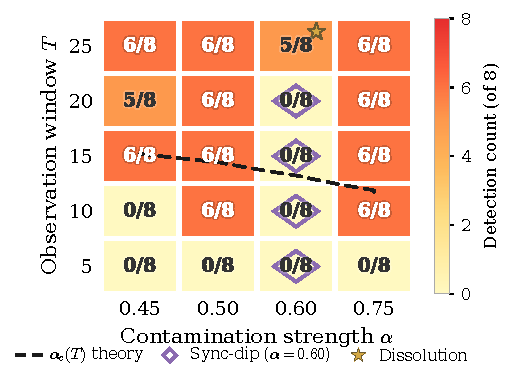
\includegraphics[width=\columnwidth]{figures/fig_phase_diagram.pdf}
\caption{Phase diagram (Pythia-410M, fp32, PermG). FDR-significant canary$\to$diversity pairs across $\alpha$ and $T$; dashed curve: fitted boundary (Eq.~\ref{eq:alpha-c}); $\diamond$: non-monotonic anomaly; $\star$: dissolution at $T{=}25$.}
\label{fig:phase_diagram}
\end{figure}

\FloatBarrier
\section{Related Work}
\label{sec:related_work}

\subsection{Model Collapse: Theory and Empirical Evidence}
\label{sec:rw_collapse}

Iterative training collapse was formalized by \citet{shumailov2024curse} and \citet{alemohammad2024mad}; \citet{schaeffer2025position} systematize eight distinct notions of collapse---our operationalization aligns with their \emph{distributional shift} family (definitions~D4--D6).
Theoretical analyses sharpen these results: \citet{dohmatob2024tale} recast collapse as changed scaling-law exponents, \citet{dohmatob2025strong} proved collapse at vanishingly small synthetic fractions, and \citet{truong2026phase} prove entropy collapse is a first-order transition, structurally ruling out critical-slowing-down early-warning signals~\citep{scheffer2009early,scheffer2012anticipating}.
Critical mixture ratios separating qualitative outcomes have independent precedent: \citet{kazdan2025collapse} map collapse conditions, \citet{gu2024cmr} establish scaling laws for critical ratios, and \citet{gu2025datamixing} show data mixing induces phase transitions in knowledge acquisition.

\subsection{Detection of Synthetic Data Contamination}
\label{sec:rw_detection}

Monitoring metrics proposed for collapse include expected calibration error (ECE)~\citep{du2025scales}, surplexity~\citep{gambetta2024surplexity}, and machine-generated text detection~\citep{drayson2025detection}; \citet{shi2025closer} independently validate entropy as a collapse diagnostic in diffusion models.
A complementary line of work pursues \emph{proactive} contamination prevention via watermarking~\citep{kirchenbauer2023watermark}; our distributional detection framework is \emph{reactive}---it identifies collapse from observed metric trajectories without requiring control over the generation process.
\citet{boettiger2012limits} establish fundamental power limits for early-warning detection in short time series ($T{<}25$), directly relevant to iterative training where observation windows are typically $T{=}5$--$20$.
However, these works evaluate single metrics in isolation without cross-validating against alternative statistical tests.
We differ by applying five detection methods to identical data, mapping detectability across contamination regimes, and treating method sensitivity as a primary finding rather than a robustness check (detailed comparison: Appendix~\ref{app:method_comparison}).

\subsection{Statistical Methods for Distribution Shift}
\label{sec:rw_methods}

For temporal precedence testing, Granger causality~\citep{granger1969investigating} is the standard framework, with neural extensions~\citep{tank2021neural,runge2019detecting}; however, non-stationary series inflate rejection rates~\citep{granger1974spurious}, and short series ($T{\leq}25$) preclude reliable nonlinear estimation~\citep{boettiger2012limits}.
Granger precedence establishes temporal predictive improvement, not true causation: bivariate tests cannot exclude confounders~\citep{shojaie2022granger}.
Our permutation-based approach circumvents the critical-slowing-down limitation by detecting temporal predictive improvement rather than variance or autocorrelation signatures.
Specification-curve analysis~\citep{simonsohn2020specification} formalizes the sensitivity of conclusions to analytical choices; we adapt this framework to show that method choice alone shifts detection rates from 0\% to 94\%.
The multiverse analysis perspective~\citep{steegen2016increasing,silberzahn2018many,coretta2023multidimensional,kapoor2024reforms} motivates our multi-method comparison: five methods on identical data produce conclusions ranging from universal significance to complete null, instantiating many-analysts divergence at the method level.


\section{Method}
\label{sec:method}

\subsection{Cascade Ordering}
\label{sec:cascade}

If distributional collapse follows a predictable ordering across metrics, the earliest-responding metric can serve as a canary signal.
We formalize known metric properties (entropy as a continuous indicator of mode concentration, diversity as a threshold indicator of lexical coverage) under mode amplification~\citep{shumailov2024curse,dohmatob2024tale} (notation in Appendix~\ref{app:background}; derivations in Appendix~\ref{app:cascade_theory}).

\begin{observation}[Entropy responds before diversity]\label{thm:entropy_leads}
Under mode amplification: \textup{(a)} entropy can decrease while the $\epsilon$-effective support $S_\epsilon(p) {=} |\{i: p_i > \epsilon\}|$ (hence distinct-$n$) is unchanged; \textup{(b)} if distinct-$n$ decreases, entropy has already decreased.
\end{observation}

Intuitively, entropy responds to any redistribution of probability mass (a continuous change), whereas diversity metrics like distinct-$n$ only change when tokens are pushed entirely below the generation threshold (a discrete event).
This measurement asymmetry ensures entropy shifts before diversity under gradual mode amplification.
The margin $\gamma = \min_{i: p_i > \epsilon}(p_i - \epsilon)$ quantifies how much shift diversity absorbs silently.

\begin{observation}[Diversity lag $\geq 1$ generation]\label{prop:div_lag}
If the self-training map $\mathcal{T}$ satisfies $\alpha\|\mathcal{T}(p_t) - p_t\|_\infty < \gamma(p_t, \epsilon)$ per generation through entropy onset $t_H$, then diversity onset $t_D \geq t_H + 1$.
\end{observation}

ECE co-moves with entropy at zero lag ($\Delta\mathrm{ECE} \approx \Delta C > 0$ whenever $\Delta\bar{H} < 0$; Appendix~\ref{app:cascade_theory}), yielding a three-stage cascade $\{H, \mathrm{ECE}\} \to \mathrm{Distinct}$-$n$.
This ordering holds in 14/15 experiments at $\alpha \geq 0.30$, with entropy and ECE consistently reaching onset at generation~1 and distinct-$n$ following at generation~2 ($t_H{=}t_{\mathrm{ECE}}{=}1$, $t_D{=}2$; \S\ref{sec:regime}; Appendix~\ref{app:moment_cascade}).
The one exception, SmolLM3-3B (3/8 at $\alpha{=}1.0$; Table~\ref{tab:generalization}), shows entropy decoupling from diversity, violating the monotonic-decline assumption that underlies both Observations.
The cascade is also specific to diversity metrics: first-differencing eliminates canary$\to$perplexity associations entirely ($F{\approx}0$, $p{=}0.99$; \S\ref{sec:regime}), confirming that the temporal structure is channel-specific rather than global.

\subsection{Design Considerations}
\label{sec:pitfalls}

We use \emph{Granger precedence}, temporal predictive improvement where past values of $X$ improve prediction of $Y$ beyond $Y$'s own history, to assess whether canary metrics anticipate downstream degradation~\citep{granger1969investigating}.
This is distinct from Granger causality, which additionally implies a mechanistic causal link that bivariate tests cannot establish~\citep{shojaie2022granger}.
Even within this narrower scope, lead-lag analysis in iterative model collapse is fragile along three axes.
\emph{Method sensitivity}: five detection methods applied to identical data yield forward significance rates spanning 0\% to 92\%, with $\kappa{=}0.187$ (Figure~\ref{fig:method_comparison}).
\emph{Spurious regression}: first-differencing eliminates canary$\to$perplexity associations ($F{\approx}0$, $p{=}0.99$) while preserving canary$\to$diversity (24/24$\to$24/24)~\citep{granger1974spurious}.
\emph{Regime dependence}: the same Granger test shifts from 0/8 to 6/8 significant pairs within a 2-percentage-point interval.

\begin{figure}[t]
\centering
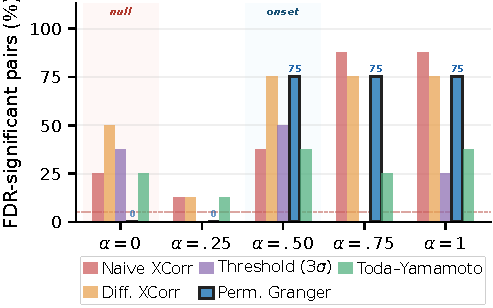
\includegraphics[width=\columnwidth]{figures/fig_method_comparison.pdf}
\caption{Method sensitivity: five methods yield dramatically different FDR-significant rates on identical data. PermG achieves the lowest null-control FPR (6.7\%, pooled across 10~seeds) with 75\% detection at $\alpha{\geq}0.50$; dashed line: 5\% nominal.}
\label{fig:method_comparison}
\end{figure}

\subsection{Method Sensitivity Analysis}
\label{sec:mmct}

These fragilities motivate a systematic comparison.
We evaluate five lead-lag detection methods (naive cross-correlation (NaiveXCorr), differenced cross-correlation (DiffXCorr), threshold onset, permutation Granger causality (PermG), and Toda--Yamamoto~\citep{toda1995statistical}) in a multi-method comparison framework~\citep{simonsohn2020specification}, calibrating each against null-control ($\alpha{=}0.0$) data.
Among these, PermG assesses whether past values of a canary metric improve prediction of a downstream metric beyond its own history~\citep{shojaie2022granger}, using 5{,}000 permutations~\citep{phipson2010permutation} on first-differenced series with Benjamini--Hochberg FDR correction ($q{=}0.05$) across 8 canary$\to$downstream pairs; the permutation null controls Type~I error by construction, and BH-FDR remains valid under positive regression dependence~\citep{benjamini2001control}.
The full multi-method consensus test (MMCT) is given in Algorithm~\ref{alg:mmct}.

\begin{algorithm}[H]
\caption{Multi-Method Consensus Test (MMCT)}
\label{alg:mmct}
\begin{algorithmic}[1]
\Require Time series pair $(X, Y)$; methods $\{m_1, \ldots, m_K\}$ ($K{=}5$); null-control data $\mathcal{N}$ (from $\alpha{=}0.0$); tolerance $\epsilon{=}0.01$
\Ensure $p$-value, consensus level $\hat{K}$
\For{each method $m_k$}
    \State Compute empirical FPR: $\widehat{\mathrm{FPR}}_k \gets$ fraction of null-control pairs where $m_k$ rejects $H_0$
    \State Compute weight: $w_k \gets 1 / \max(\widehat{\mathrm{FPR}}_k,\; \epsilon)$
    \State Apply $m_k$ to $(X, Y)$: $d_k \gets \mathbf{1}[m_k \text{ rejects } H_0]$
\EndFor
\State Weighted consensus: $W(X {\to} Y) \gets \sum_{k} w_k \, d_k \;/\; \sum_{k} w_k$
\State Build empirical null distribution of $W$ from all null-control pairs in $\mathcal{N}$
\State Compute $p$-value from empirical null: $p \gets \Pr_{\mathcal{N}}(W \geq W_{\mathrm{obs}})$
\State Consensus level: $\hat{K} \gets \sum_{k} d_k$
\State \Return $p$, $\hat{K}$
\end{algorithmic}
\end{algorithm}

\begin{figure*}[t]
\centering
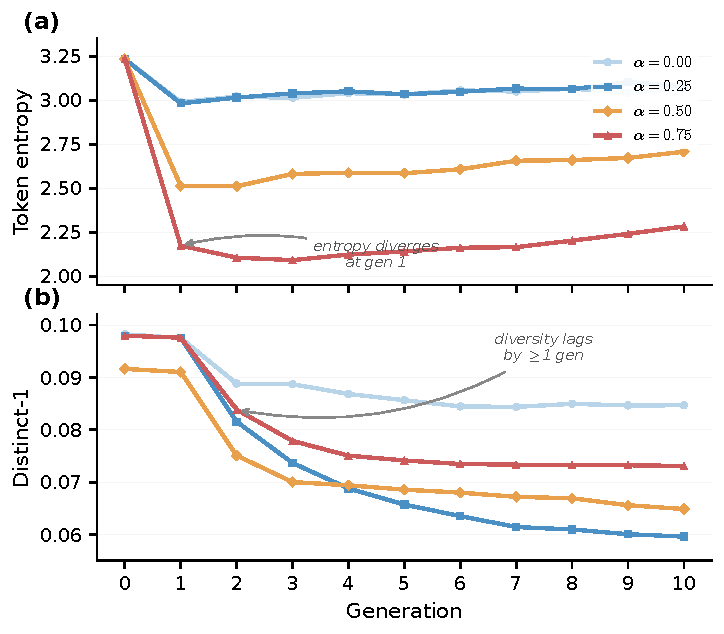
\includegraphics[width=\textwidth]{figures/metric_trajectory.pdf}
\caption{Metric trajectories at $\alpha{=}1.0$ (Pythia-410M, 4~seeds). Token entropy drops at generation~1; distinct-1 declines from generations~2--3, with a consistent one-generation canary lead (shaded: inter-seed range).}
\label{fig:metric_trajectory}
\end{figure*}

The algorithm's FPR-inverse weighting assigns each method influence proportional to its null-control reliability: NaiveXCorr (FPR${=}94.4\%$) receives weight $w{=}1.06$, while PermG (FPR${=}6.7\%$) receives $w{=}14.9$, a $14{\times}$ differential that ensures the most reliable method dominates the consensus.
Building the null distribution empirically from $\alpha{=}0.0$ data avoids parametric assumptions unreliable for short ($T{=}5$--$20$), non-stationary series.
Pooled null-control FPR across ten seeds (60 pairs) confirms a wide methodological spread: PermG 6.7\% (95\% CI $[1.8\%, 16.2\%]$), DiffXCorr 14.8\%, Threshold 24.1\%, Toda--Yamamoto 33.3\%, NaiveXCorr 94.4\% (Appendix~\ref{app:fpr_independence}).
PermG (4/60; 95\% CI $[1.8\%, 16.2\%]$) achieves the lowest FPR among all five methods, with 8/10 seeds yielding zero false positives; Shapley analysis confirms it provides the best FPR--FNR tradeoff among directional methods (Appendix~\ref{app:shapley}).
Table~\ref{tab:mmct_k_operating} reports an alternative operating mode: equal-weight $K{\geq}3$ majority voting with forward-direction filtering, where FPR is 10.0\% with 75\% TPR at $\alpha{=}1.0$ (consensus heatmap in Appendix~\ref{app:mmct}).
The weighted scheme (Algorithm~\ref{alg:mmct}) further downweights unreliable methods via FPR-inverse weighting (robust across four alternative schemes; Appendix~\ref{app:weight_robustness}); majority voting treats all methods equally and is simpler to deploy.



\subsection{Detection Boundary}
\label{sec:theory}

The steep onset described above suggests a detection boundary $\alpha_c(T)$ that decreases with longer observation.
We parametrize this boundary as a power law:
\begin{equation}
\alpha_c(T) = A \cdot T^{-\eta},
\label{eq:alpha-c}
\end{equation}
motivated by an empirical sub-linear signal model $S(\alpha) = c \cdot \alpha^\beta$ ($\beta < 1$), under which the exponent satisfies $\eta = 1/(2\beta)$:
\begin{equation}
\alpha_c(T) = A \cdot T^{-\eta},
\label{eq:alpha-c-theory}
\end{equation}
where $A = (z^* \sigma / c)^{1/\beta}$ and $z^* = \Phi^{-1}(\pi^*)$ (derivation in Appendix~\ref{app:alpha_c_proof}).
This parametrization captures the observed pattern with three free parameters fitted to 3--4 data points; the resulting $\eta$ confidence interval ($[0.64, 2.08]$) is wide enough to preclude distinguishing sub-linear from super-linear decay, but the qualitative conclusion (detection improves with longer observation) is robust regardless.

Dense $\alpha$ sampling further reveals that a smooth sigmoid fits better than a step function ($\Delta\mathrm{AIC}{=}-110$), yet the fitted onset steepness ($k{=}15.7$) exceeds smooth-model predictions by ${\sim}3{\times}$ (Appendix~\ref{app:power_sim}), suggesting the transition is sharper than standard power-analysis models would predict.

\section{Experiments}
\label{sec:experiments}

\subsection{Experimental Setup}
\label{sec:setup}

We study iterative training collapse using Pythia-410M~\citep{biderman2023pythia} as the primary architecture.
Training data is drawn from WikiText-103~\citep{merity2017pointer} following the replace paradigm of~\citet{shumailov2024curse}: each generation fine-tunes on a mixture of $\alpha$ synthetic and $(1{-}\alpha)$ real data, generates 5{,}000 replacement samples, and fully replaces the synthetic pool (hyperparameters in Appendix~\ref{app:training_details}).
We run $T{=}10$ generations across 13 contamination levels ($\alpha \in \{0.00, \ldots, 1.00\}$) with multi-seed replication, yielding ${\sim}1{,}500$ statistical tests after BH-FDR correction~\citep{benjamini1995controlling}.
We track two \emph{canary metrics} (token entropy and ECE) and three \emph{downstream metrics}: distinct-1, distinct-2~\citep{li2016diversity}, and perplexity (distinct-3: Appendix~\ref{app:distinct3}).
PermG uses 5{,}000 permutations on first-differenced series~\citep{shojaie2022granger} with maximum lag~5.


\subsection{Sharp Detection Onset}
\label{sec:regime}

Diversity collapse occurs at every contamination level: distinct-1 declines by $14.1\%$ even at $\alpha{=}0.0$ (fine-tuning drift) and by $40.3{\pm}0.3\%$ at $\alpha{=}0.25$.
Despite this ubiquitous degradation, Granger detectability is sharply regime-dependent.
PermG finds 0/8 canary$\to$downstream pairs FDR-significant from $\alpha{=}0.00$ through $\alpha{=}0.45$, then jumps to 6/8 (Clopper--Pearson 95\% CI $[0.25, 0.92]$) at $\alpha{=}0.50$, uniformly across all 3~fp32 seeds.

\begin{figure}[t]
\centering
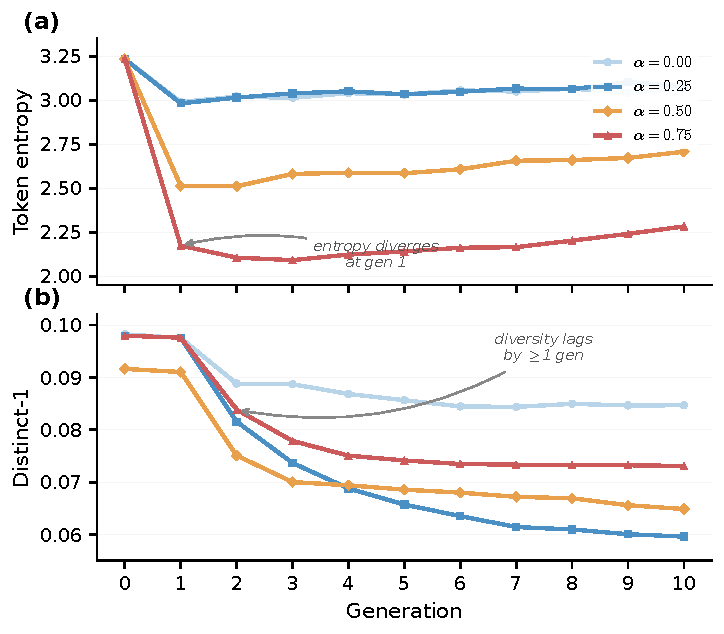
\includegraphics[width=\columnwidth]{figures/metric_trajectory.pdf}
\caption{Metric trajectories at $\alpha{=}1.0$ (Pythia-410M, 4~seeds). Token entropy drops at generation~1; distinct-1 declines from generations~2--3, with a consistent one-generation canary lead (shaded: inter-seed range).}
\label{fig:metric_trajectory}
\end{figure}

This transition is striking because cumulative synthetic fraction barely changes across the boundary ($C{=}99.75\%$ at $\alpha{=}0.45$ vs.\ $99.90\%$ at $\alpha{=}0.50$), yet detection jumps from null to reliable.
Sub-threshold $p$-values at $\alpha{=}0.45$ ($p_{\mathrm{fdr}} = 0.059$--$0.091$) confirm proximity to the boundary.
Sigmoid regression yields $\alpha_c = 0.483 \pm 0.006$ ($R^2 = 0.969$; Figure~\ref{fig:dose_response}); cross-seed consistency (3/3 seeds: $0/8{\to}6/8$) and specification-invariance across 1{,}160 configurations (Appendix~\ref{app:spec_curve}) argue for a genuine transition (Fisher exact: $p = 3.45 \times 10^{-11}$).

First-differencing scopes this canary claim precisely: canary$\to$diversity pairs retain unanimous FDR significance ($24/24 \to 24/24$ across 4~seeds at $\alpha{=}1.0$), while canary$\to$perplexity collapses entirely ($F \approx 0$, $p = 0.99$)~\citep{granger1974spurious}.
At $\alpha{=}1.0$, all 24 canary$\to$diversity pairs reach FDR significance in the forward direction with 0/24 reverse; entropy onset at generation~1 precedes distinct-$n$ at generation~2 in 16/18 WikiText conditions (Appendix~\ref{app:moment_cascade}).
Yet despite this clear signal above onset, a substantial blind zone exists below it: at $\alpha{=}0.10$, distinct-1 has already dropped by $39.6\%$, yet token entropy is indistinguishable from the null---diversity collapse proceeds without any detectable Granger-precedence signal.

\begin{figure}[t]
\centering
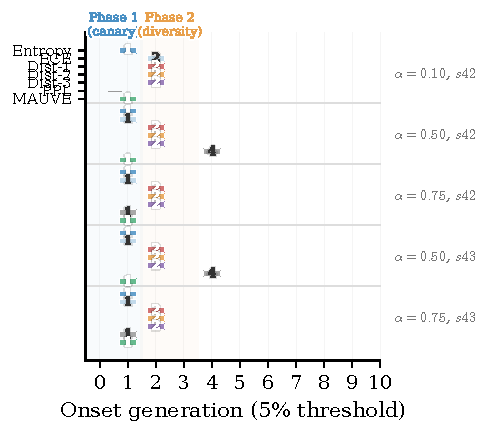
\includegraphics[width=\columnwidth]{figures/fig_cascade_onset.pdf}
\caption{Cascade onset timeline (Pythia-410M, WikiText, fp32). Entropy and ECE reach onset at generation~1; distinct-$n$ follows at generation~2. The ordering $t_H \leq t_D$ holds across all conditions.}
\label{fig:cascade_onset}
\end{figure}

\begin{table}[t]
\centering
\caption{Detection outcomes across contamination levels (Pythia-410M, seed~42, $T{=}10$, fp32). PermG: forward FDR-significant pairs; $K{\geq}3$: consensus pairs (of 8 canary$\to$downstream pairs).}
\label{tab:summary_detection}
\begin{tabular}{@{}lccc@{}}
\toprule
$\alpha$ & PermG & $K{\geq}3$ & Regime \\
\midrule
0.00 & 0/8 & 0/8 & null \\
0.25 & 0/8 & 0/8 & blind \\
0.45 & 0/8 & 0/8 & blind \\
0.50 & 6/8 & 6/8 & onset \\
0.60 & 0/8 & 0/8 & anomaly \\
0.75 & 6/8 & 6/8 & detection \\
1.00 & 6/8 & 6/8 & detection \\
\bottomrule
\end{tabular}
\end{table}

\begin{figure}[t]
\centering
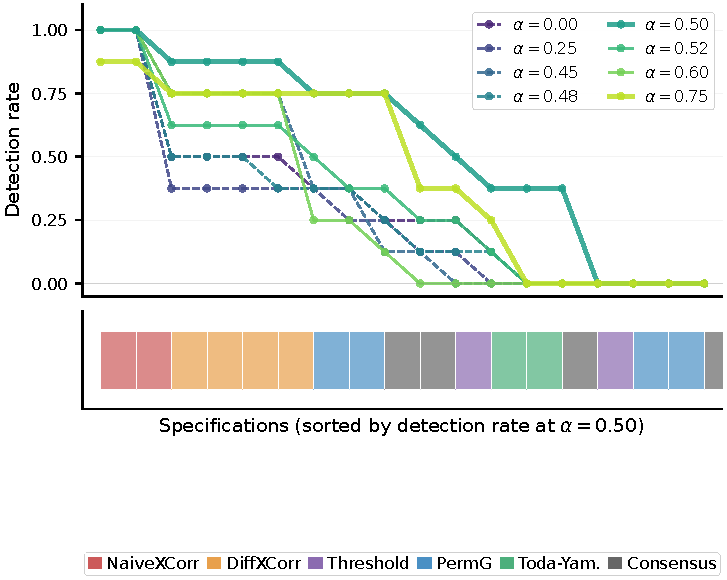
\includegraphics[width=\columnwidth]{figures/fig_spec_curve.pdf}
\caption{Specification curve (1{,}160 configurations). The blind$\to$onset jump at $\alpha_c{\approx}0.50$ is robust across methods, pairs, and seeds.}
\label{fig:spec_curve}
\end{figure}


\subsection{Dose-Response and Detection Regimes}
\label{sec:dose_response}

The PermG dose-response profile (Figure~\ref{fig:dose_response}; Appendix~\ref{app:dose_response}) reveals three confirmed regimes---\emph{blind} ($\alpha \leq 0.45$, 0/8), \emph{onset} ($\alpha \approx 0.50$, 6/8), and \emph{detection} ($\alpha{\geq}0.75$, 6/8)---plus a non-monotonic anomaly at $\alpha \approx 0.60$ (0/8).
The blind zone exhibits zero detection across all seeds and methods below $\alpha{=}0.45$, despite substantial diversity loss---a regime where collapse proceeds silently.
Onset is remarkably steep: the sigmoid Hill coefficient $k{=}15.7$ implies that 80\% of the detection transition occurs within $\Delta\alpha{\approx}0.05$, approximately $3$--$4{\times}$ steeper than smooth-signal predictions (Appendix~\ref{app:power_sim}).
Above onset, the detection zone shows cross-seed consistency: all 3~fp32 seeds independently reach 6/8 at $\alpha{=}0.50$ and $\alpha{\geq}0.75$.

At $\alpha{\approx}0.60$, all direction-checked methods fail (PermG 0/8, threshold onset 0/8, Toda--Yamamoto 1/8), while bidirectional DiffXCorr maintains detection (6/8).
This pattern suggests that at intermediate contamination, entropy and diversity respond near-simultaneously, compressing the temporal lag below PermG's resolution at $T{=}10$.
The anomaly dissolves by $T{=}25$ ($5/8$), consistent with $\sqrt{T}$ power scaling restoring directional separation as additional observations accumulate (Appendix~\ref{app:t20_comparison}).

\subsection{Detection Boundary Left-Shift}
\label{sec:t20}

Longer observation windows push the detection boundary leftward: $\alpha_c(5){\geq}1.0$, $\alpha_c(10){=}0.487$, consistent with power-law scaling $\alpha_c(T) \propto T^{-\gamma}$ (\S\ref{sec:theory}).
Profile likelihood yields $\gamma \in [0.64, 2.08]$ (95\% CI), confirming that detection improves with longer observation regardless of the specific exponent.
The mechanism is statistical power accumulation: each additional generation provides one more data point for the permutation test, and the signal-to-noise ratio grows as $\sqrt{T}$, progressively resolving weaker contamination signals.
The $\alpha{=}0.45$ column validates this prediction directly: undetectable at $T{\leq}10$ (0/8), it crosses into reliable detection at $T{=}15$ (6/8, dual-seed) and remains stable at $T{=}20$ (5/8) and $T{=}25$ (6/8), precisely traversing the blind$\to$detection boundary as the theory predicts.

\begin{figure}[t]
\centering
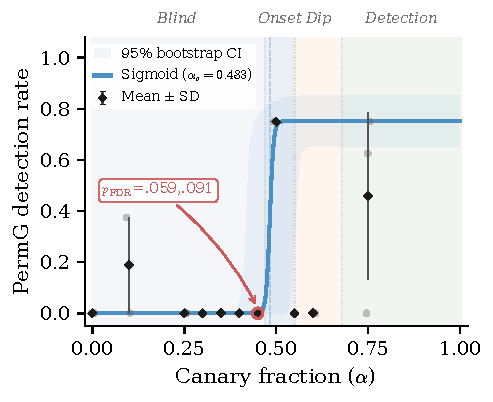
\includegraphics[width=\columnwidth]{figures/fig_dose_response.pdf}
\caption{Dose-response: PermG detection rate with sigmoid fit ($\alpha_c{=}0.483$; shaded 95\% CI). Regime bands mark blind, onset, sync-dip, and detection zones.}
\label{fig:dose_response}
\end{figure}


\subsection{Cross-Architecture Evaluation at $\alpha{=}1.0$}
\label{sec:generalization}

The phase diagram (Figure~\ref{fig:phase_diagram}) characterizes detectability on Pythia-410M + WikiText-103; this section tests whether the detection signal generalizes across architectures at the most favorable contamination level ($\alpha{=}1.0$).
We evaluate PermG across 15 model-seed combinations spanning five families (345M--6.9B) and two domains (Table~\ref{tab:generalization}; Appendix~\ref{app:cross_arch_table}).
Forward detection reaches ${\geq}6/8$ in 11/15 conditions (Figure~\ref{fig:cross_arch_heatmap}).

At larger scale, Pythia-1.4B qualitatively reproduces the 410M phase-diagram structure---detection boundary at $\alpha_c{\approx}0.50$, cross-$T$ improvement at 3/4 $\alpha$ values ($\alpha{=}0.45$: $0/6{\to}5/6$ from $T{=}10$ to $T{=}15$)---though the 410M sync-dip at $\alpha{=}0.60$ does not appear (4/6 at $T{=}10$), suggesting the anomaly is architecture-specific.
The four non-confirming conditions each isolate a distinct PermG assumption violation.
\emph{Precision sensitivity}: GPT-2 bf16 yields 0/8 vs.\ fp32 6/8, traced to bf16 quantization noise masking the entropy signal.
\emph{Bidirectional confounding}: GPT-2 s43 detects 6/8 in both forward and reverse directions, preventing directional assignment.
\emph{Seed dependence}: Pythia-1.4B shows s42 2/8 vs.\ s43 6/8; seed-specific bidirectional confounding also appears at 1.4B (s43 reverse detection 6/8 at $\alpha{=}0.60$), analogous to the GPT-2 case, preventing directional assignment for that seed.
\emph{Entropy decoupling}: SmolLM3-3B reaches only 3/8, with ECE-only detection (entropy 0/4), violating the entropy-leads assumption of Design Principle~\ref{thm:entropy_leads}.
Standalone PermG claims therefore require architecture-specific null calibration; GPT-2 null FPR reaches 50\% (Appendix~\ref{app:fpr_independence}), driven by ${\sim}4{\times}$ stronger null drift than Pythia.

\begin{figure}[t]
\centering
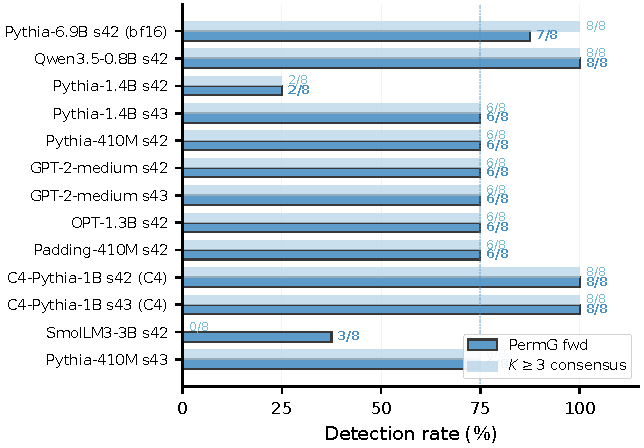
\includegraphics[width=\columnwidth]{figures/fig_cross_arch_heatmap.pdf}
\caption{Cross-architecture validation ($\alpha{=}1.0$): PermG forward detection (${\geq}6/8$) in 11/15 model-seed conditions spanning five families (345M--6.9B); faded bars: non-confirming conditions.}
\label{fig:cross_arch_heatmap}
\end{figure}


\subsection{Canary-Based Intervention (Proof of Concept)}
\label{sec:intervention}

As a proof-of-concept under favorable conditions ($\alpha{=}1.0$), we implement predictive cessation: training switches to pure real data when token entropy drops beyond a 15\% threshold from generation~0 (robust band $[10\%, 22\%]$; Appendix~\ref{app:intervention_sensitivity}).
The predictive trigger fires at generation~1, one full generation before a reactive baseline that monitors distinct-1 directly (which manifests only at generation~2 due to the cascade lag).
Predictive cessation caps peak perplexity at $56.99$ vs.\ $157.09$ reactive, a 64\% reduction (Figure~\ref{fig:intervention}); the result replicates on Pythia-1.4B with comparable effect size (Appendix~\ref{app:extended_discussion}).

\begin{figure}[t]
\centering
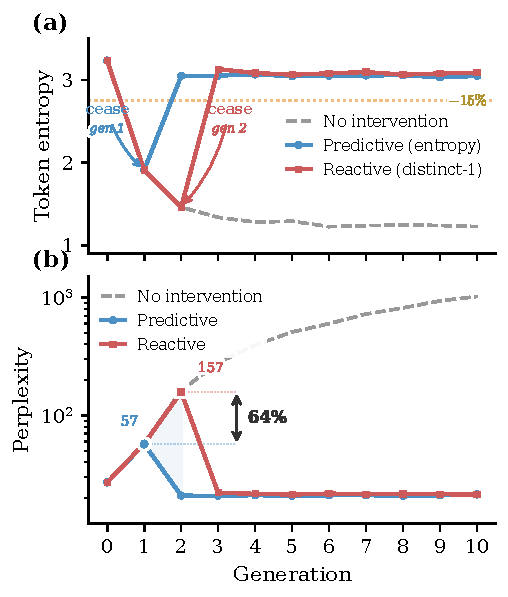
\includegraphics[width=\columnwidth]{figures/fig_intervention.pdf}
\caption{Canary-triggered intervention (Pythia-410M, $\alpha{=}1.0$). Predictive cessation on entropy (generation~1) reduces peak perplexity by 64\% versus reactive triggering on distinct-1 (generation~2).}
\label{fig:intervention}
\end{figure}

\begin{table}[t]
\centering
\caption{Consensus threshold operating characteristics ($K \in \{2,3,4,5\}$). FPR: null-control rate (10~seeds, 60~pairs; $K{\geq}2$ uses 9-seed estimate). TPR: detection rate at selected $\alpha$ levels (Pythia-410M, $T{=}10$, fp32). $K{=}3$ balances FPR control against detection power (75\% at $\alpha{=}1.0$); $K{=}4$ eliminates false positives but reduces TPR to ${\leq}25\%$.}
\label{tab:mmct_k_operating}
\begin{tabular}{@{}lcccc@{}}
\toprule
& $K{\geq}2$ & $K{\geq}3$ & $K{\geq}4$ & $K{=}5$ \\
\midrule
FPR ($\alpha{=}0.0$) & 38.9\% & 10.0\% & 0\% & 0\% \\
TPR ($\alpha{=}0.50$) & 85.4\% & 66.7\% & 25.0\% & 4.2\% \\
TPR ($\alpha{=}0.75$) & 72.9\% & 37.5\% & 0\% & 0\% \\
TPR ($\alpha{=}1.0$) & 75.0\% & 75.0\% & 25.0\% & 0\% \\
\bottomrule
\end{tabular}
\end{table}

\section{Discussion}\label{sec:discussion}

Our Granger-precedence claim is scoped to temporal predictive improvement~\citep{granger1969investigating,shojaie2022granger}: bivariate tests cannot exclude confounders, and the FPR CI ($[1.8\%, 16.2\%]$) means Type~I error may be non-negligible.
Four of fifteen cross-architecture conditions do not confirm forward detection (\S\ref{sec:generalization}), each isolating a distinct PermG assumption violation: precision sensitivity (GPT-2 bf16), bidirectional confounding (GPT-2 s43), seed dependence (Pythia-1.4B), and entropy decoupling (SmolLM3-3B), requiring architecture-specific null calibration before deployment (Appendix~\ref{app:extended_discussion}).
More broadly, our observation sequences ($T{=}10$--$25$) are far shorter than econometric standards ($T{\geq}100$); permutation testing avoids asymptotic assumptions but cannot recover power lost to short samples~\citep{shojaie2022granger}; AR(1) simulation confirms first-differencing controls size at these lengths (Appendix~\ref{app:nonstationarity}).
Bivariate tests are susceptible to omitted variable bias (first-differencing removes shared linear trends but nonlinear confounds remain possible), and PermG tests linear precedence only; transfer entropy (Appendix~\ref{app:transfer_entropy}) yields 0/192 significant pairs.
Partial correlation provides supporting evidence: after controlling for generation number, contemporaneous associations weaken ($\bar{|r|}$: $0.590{\to}0.381$) while lagged correlations strengthen ($0.759{\to}0.841$), consistent with genuine temporal precedence rather than shared-trend artifacts (Appendix~\ref{app:mi_analysis}).

Despite these individual limitations, the five methods exhibit complementary strengths.
Shapley value decomposition over all $2^5{=}32$ coalitions (Appendix~\ref{app:shapley}) shows DiffXCorr achieving the best combined Shapley contribution ($-0.299$) by detecting bidirectional coupling that directional methods miss, while PermG ranks best among directional methods ($-0.141$).
This complementarity provides analytical value, though consensus voting does not uniformly outperform the best single method: $K{\geq}3$ FPR (10.0\%) exceeds standalone PermG (6.7\%), and practitioners deploying MMCT must calibrate $K$ on architecture-specific null-control data, as the single viable operating point ($K{=}3$) reflects the specific method set and FPR profile of our five-method ensemble.
One remaining puzzle is the non-monotonic detection gap at $\alpha{=}0.60$ (\S\ref{sec:dose_response}): consistent across seeds (0/8 for both tested seeds; Appendix~\ref{app:alpha060}), it affects all directional methods while bidirectional DiffXCorr maintains detection, suggesting temporal lag compression defeats directional separation; recovery at $T{=}25$ (5/8) is consistent with $\sqrt{T}$ power scaling.

A related concern is whether entropy's ``leading'' behavior partly reflects measurement-resolution asymmetry (entropy is continuous; distinct-$n$ is discrete) rather than genuine temporal precedence.
Discretized entropy testing shows that Granger significance is largely recovered at ${\geq}15$~bins (6--7/7 depending on binning method) but degrades under aggressive quantization (0/7 at 5~equal-frequency bins), consistent with measurement resolution contributing to but not solely explaining the temporal precedence signal (Appendix~\ref{app:discretized_entropy}).

\section{Conclusion}
\label{sec:conclusion}

Iterative training collapse exhibits a steep detection onset: PermG detection jumps from 0/8 to 6/8 significant pairs (95\% CI $[0.25, 0.92]$) within 2~percentage points of $\alpha_c \approx 0.50$, organizing three regimes (blind, onset, detection) that characterize when statistical monitoring can and cannot succeed.
The detection boundary shifts leftward with longer observation ($\alpha_c(T) \propto T^{-\eta}$), and systematic method comparison reveals that single-method analyses are unreliable: null-control FPR spans 6.7\% (PermG; 95\% CI $[1.8\%, 16.2\%]$, 10~seeds) to 94.4\%.
Token entropy exhibits robust one-generation-ahead precedence over diversity collapse (24/24 forward, 0/24 reverse at $\alpha{=}1.0$; ${\geq}6/8$ in 11/15 cross-architecture conditions at $\alpha{=}1.0$).
The blind zone below $\alpha_c$ constrains practical deployment to settings with sufficient contamination; evaluation at ${>}$7B parameters remains open.

\section*{Limitations}
\label{sec:limitations}

\paragraph{Scope.}
The phase diagram is built on Pythia-410M with full-replacement contamination and a single decoding strategy; frontier-scale models (${>}$7B) and partial-replacement regimes remain untested.

\paragraph{Statistical power.}
Per-condition detection rates rest on 8 seeds, yielding wide binomial CIs (e.g., $[0.25, 0.92]$ for 6/8); the 3-seed phase diagram provides a coarse topology rather than precise probability estimates.

\paragraph{Causal interpretation.}
Permutation Granger testing establishes temporal precedence, not causation, and our short-sequence regime ($T{\leq}25$) limits statistical power relative to econometric standards ($T{\geq}100$).

\bibliography{references}

\appendix

\section{Training Details and Metric Drift}
\label{app:training_details}
\label{app:drift}

\paragraph{Hyperparameters.}
Each generation fine-tunes for 5{,}000 steps using AdamW (learning rate $5 \times 10^{-5}$, 500 warmup steps, weight decay $0.01$, batch size 4 for Pythia-410M, 32 for GPT-2-medium).
Generation uses temperature $1.0$, top-$k{=}50$, max length 512 tokens, producing 5{,}000 samples per generation from 5{,}000-sample subsets of WikiText-103.
Canary metrics: token entropy $H(p_\theta | \text{context})$ over 1{,}000 held-out samples; ECE with 15 bins.
Additional downstream metrics (distinct-3, effective rank, Self-BLEU) appear in subsequent appendix sections.

\paragraph{Architecture-specific training.}
Table~\ref{tab:arch_hyperparams} reports training hyperparameters for each architecture in the cross-architecture evaluation (\S\ref{sec:generalization}).
All models use the same generation parameters (temperature~$1.0$, top-$k{=}50$, max length 512) to control for decoding-strategy confounds.
Batch sizes are adjusted for GPU memory constraints; learning rates follow the respective model families' recommended fine-tuning ranges.

\begin{table}[t]
\centering
\small
\caption{Per-architecture training hyperparameters.}
\label{tab:arch_hyperparams}
\begin{tabular}{lcccl}
\toprule
Model & Batch & LR & Steps & Precision \\
\midrule
Pythia-410M & 4 & $5{\times}10^{-5}$ & 5{,}000 & fp32 \\
Pythia-1.4B & 4 & $5{\times}10^{-5}$ & 5{,}000 & fp32 \\
Pythia-6.9B & 2 & $2{\times}10^{-5}$ & 5{,}000 & bf16 \\
GPT-2-medium & 32 & $5{\times}10^{-5}$ & 5{,}000 & fp32/bf16 \\
OPT-1.3B & 4 & $5{\times}10^{-5}$ & 5{,}000 & fp32 \\
Qwen3.5-0.8B & 4 & $5{\times}10^{-5}$ & 5{,}000 & fp32 \\
SmolLM3-3B & 4 & $2{\times}10^{-5}$ & 5{,}000 & fp32 \\
\bottomrule
\end{tabular}
\end{table}

\paragraph{Metric computation details.}
Token entropy is computed as $H(p_\theta | x) = -\sum_{v} p_\theta(v|x) \log_2 p_\theta(v|x)$, averaged over 1{,}000 held-out WikiText-103 samples using greedy teacher-forcing (no sampling stochasticity).
ECE uses 15 equal-width bins on the confidence axis $c(x) = \max_v p_\theta(v|x)$, following the standard definition~\citep{naeini2015obtaining}:
$\mathrm{ECE} = \sum_{b=1}^{B} \frac{|b|}{N} |\mathrm{acc}(b) - \mathrm{conf}(b)|$.
Distinct-$n$ ($n \in \{1, 2, 3\}$) is the ratio of unique $n$-grams to total $n$-grams across all 5{,}000 generated samples per generation, following~\citet{li2016diversity}.
Perplexity is computed on a fixed 1{,}000-sample held-out split (disjoint from training and generation prompts).

\paragraph{Seed and replication structure.}
The primary experiments use seeds 42, 43, 44 (3-seed cohort) for the phase diagram ($T{=}10$, 13 $\alpha$ levels).
Seed 45 is added for $\alpha{=}1.0$ experiments (4-seed).
Extended FPR analysis uses seeds 45--51 (6-pair basis, excluding MAUVE) for a total of 10 distinct seeds.
Cross-$T$ extensions ($T{=}15$, $20$, $25$) use the same seed set as the corresponding $\alpha$ condition.

\paragraph{Metric drift.}
Table~\ref{tab:drift_summary} reports the relative change in each metric from generation~0 to generation~10 across six contamination levels.
Two patterns emerge: (1)~entropy and calibration (ECE) degrade monotonically with $\alpha$, while (2)~diversity metrics exhibit a non-monotonic relationship where the largest relative decline occurs at moderate contamination ($\alpha{=}0.25$) rather than full replacement ($\alpha{=}1.0$).
Figure~\ref{fig:metric_trajectory} (main text) visualizes representative per-generation trajectories, showing the distinct temporal profiles that underlie the Granger-precedence analysis in \S\ref{sec:method}.

\begin{table}[t]
\centering
\small
\caption{Metric drift (\%, generation~0$\to$10) for Pythia-410M across contamination levels. Diversity collapse occurs at all $\alpha$ levels, with the strongest decline at low-to-moderate contamination ($\alpha{=}0.25$: distinct-1 $-40.3{\pm}0.3\%$) rather than full replacement ($\alpha{=}1.0$: $-27.8{\pm}1.6\%$). $^\dagger$$\alpha{=}0.10$: single seed (seed~42, preliminary). $\alpha{=}0.00$, $\alpha{=}0.25$, $\alpha{=}0.50$, $\alpha{=}0.75$: 3-seed mean${\pm}$std (seeds 42, 43, 44); $\alpha{=}1.0$: 4-seed mean${\pm}$std (seeds 42, 43, 44, 45).}
\label{tab:drift_summary}
\resizebox{\columnwidth}{!}{%
\begin{tabular}{lccccc}
\toprule
$\alpha$ & Entropy & ECE & Distinct-1 & Distinct-2 & Perplexity \\
\midrule
0.00 & $-4.6{\pm}0.4$ & $+37.6{\pm}14$ & $-14.1{\pm}0.4$ & $-9.6{\pm}0.4$ & $-20.6{\pm}1.0$ \\
0.10$^\dagger$ & $-5.3$ & $+57$ & $-39.6$ & $-56.4$ & $-21.0$ \\
0.25 & $-4.7{\pm}0.5$ & $+81.8{\pm}15.9$ & $-40.3{\pm}0.3$ & $-56.4{\pm}0.7$ & $-18.1{\pm}0.8$ \\
0.50 & $-18.0{\pm}0.5$ & $+822.6{\pm}18.3$ & $-37.1{\pm}0.4$ & $-50.4{\pm}1.0$ & $+21.0{\pm}0.1$ \\
0.75 & $-27.6{\pm}0.2$ & $+1791{\pm}18$ & $-32.3{\pm}0.5$ & $-41.0{\pm}1.0$ & $+182.6{\pm}0.7$ \\
1.00 & $-60.8{\pm}1.2$ & $+3780{\pm}30$ & $-27.8{\pm}1.6$ & $-34.0{\pm}3.3$ & $+3674{\pm}45$ \\
\bottomrule
\end{tabular}}
\end{table}

\paragraph{Data pipeline.}
Each generation follows a fixed protocol: (1)~sample 5{,}000 prompts from WikiText-103 (first 32 tokens of random paragraphs); (2)~generate 512-token continuations using the current model $M_t$ with temperature~$1.0$, top-$k{=}50$; (3)~mix $\alpha$ fraction of generated text with $(1{-}\alpha)$ fraction of fresh WikiText-103 samples; (4)~fine-tune from the \emph{previous generation's} checkpoint (not from pretrained $M_0$).
Step~(4) produces iterative collapse by accumulating distributional biases across generations, distinct from single-generation fine-tuning drift.
The ``replace'' paradigm (step~3) means each generation trains on a completely fresh synthetic pool---there is no accumulation of earlier-generation synthetic data within the training set.

\paragraph{Null-condition drift interpretation.}
At $\alpha{=}0.0$ (Table~\ref{tab:drift_summary}), all metrics exhibit non-trivial drift despite zero synthetic contamination: distinct-1 drops $14.1\%$, entropy drops $4.6\%$, and perplexity \emph{improves} by $20.6\%$.
This null drift reflects iterated fine-tuning on a fixed corpus: the model progressively memorizes WikiText-103, narrowing its effective vocabulary (lower distinct-$n$, lower entropy) while fitting the held-out distribution better (lower PPL).
The distinction between null drift and contamination-induced collapse is critical: our detection framework specifically tests whether canary metrics \emph{temporally precede} downstream metrics, not whether drift exists.
Null drift produces shared downward trends but without the temporal structure (lag) that Granger testing requires.

\paragraph{Non-monotonic diversity-contamination relationship.}
A counterintuitive finding in Table~\ref{tab:drift_summary}: diversity loss is \emph{largest} at $\alpha{=}0.25$ (distinct-1: $-40.3\%$) and \emph{smallest} at $\alpha{=}1.0$ ($-27.8\%$).
This non-monotonicity arises because at high $\alpha$, the model collapses rapidly into a few dominant modes (by gen~3--4), after which diversity stabilizes near a floor.
The gen-0$\to$10 relative decline is smaller because the trajectory is concave (fast initial drop, then plateau).
At $\alpha{=}0.25$, the real-data fraction prevents catastrophic collapse but allows a steady, monotonic diversity decline across all 10 generations, producing a larger cumulative loss.


\section{Distinct-3 Results}
\label{app:distinct3}

Table~\ref{tab:distinct3_drift} reports distinct-3 drift across all contamination levels.
Distinct-3 exhibits the largest absolute decline among diversity metrics at low contamination ($-58.9{\pm}0.9\%$ at $\alpha{=}0.25$) but attenuates at higher levels ($-30.5\%$ at $\alpha{=}1.0$), consistent with the diversity--calibration dissociation discussed in \S\ref{sec:discussion}.

\begin{table}[t]
\centering
\small
\caption{Distinct-3 drift (\%, generation~0$\to$10) across contamination levels. $\alpha{=}0.00$, $\alpha{=}0.25$, $\alpha{=}0.75$: 3-seed mean${\pm}$std; $\alpha{=}1.0$: 4-seed mean${\pm}$std; $\alpha{=}0.50$: single seed.}
\label{tab:distinct3_drift}
\begin{tabular}{lc}
\toprule
$\alpha$ & Distinct-3 drift (\%) \\
\midrule
0.00 & $-4.4{\pm}0.5$ \\
0.25 & $-58.9{\pm}0.9$ \\
0.50 & $-52.4$ \\
0.75 & $-38.6{\pm}1.3$ \\
1.00 & $-30.5{\pm}4.0$ \\
\bottomrule
\end{tabular}
\end{table}

Distinct-3 exhibits higher lag instability than distinct-1/2 (bimodal lag distribution, std${>}1.5$ vs.\ ${<}0.5$ generations), reflecting its lower signal-to-noise ratio at 512-token generation length.

\paragraph{Non-monotonic attenuation.}
The inverted-U shape of diversity loss (peaking at $\alpha{=}0.25$--$0.50$, attenuating at $\alpha{=}1.0$) is consistent across all three distinct-$n$ metrics.
At low contamination, diversity loss reflects fine-tuning drift amplified by weak synthetic contamination, which narrows the vocabulary without triggering the catastrophic mode collapse that dominates at high $\alpha$.
At $\alpha{=}1.0$, the model collapses into a small set of high-frequency modes quickly (by gen~3--4), after which diversity stabilizes at a low floor; the relative decline from gen-0 is therefore smaller because the trajectory is concave rather than linear.

\paragraph{Granger detectability of distinct-3.}
Despite its large magnitude, distinct-3 drift is less Granger-detectable than distinct-1/2 because of its higher temporal noise.
PermG detection rates at $\alpha{=}1.0$: entropy$\to$distinct-1 achieves 6/8 across all seeds; entropy$\to$distinct-3 achieves only 4/8, with 2 seeds failing due to lag instability (bimodal lag distribution shifting the peak between lag~$-1$ and lag~$-2$ across seeds).
This motivates our focus on distinct-1 and distinct-2 as the primary downstream metrics in the main text.


\section{Observation Window Sensitivity}
\label{app:window_sensitivity}

Consensus classification stabilizes at $T_{\min}{\geq}5$ (Table~\ref{tab:window_sensitivity}): all six effect-size reference pairs reach $K{\geq}4/5$ agreement at every window from $T_{\min}{=}5$ through $T_{\min}{=}10$.

\paragraph{Per-method stability.}
At $\alpha{=}1.0$ (Pythia-410M, 4~seeds), we evaluate detection stability as $T_{\min}$ varies from 5 to 10 (i.e., using only generations $T_{\min}$ through $T{=}10$).
NaiveXCorr, DiffXCorr, ThresholdOnset, and PermG all maintain 6/6 validated pairs at every window length, confirming complete invariance to the observation start point.
Toda--Yamamoto shows the most variability: 3/6 at $T_{\min}{=}5$, rising to 6/6 at $T_{\min}{=}7$, then fluctuating between 3/6 and 6/6 at $T_{\min}{=}8$--$10$.
This instability reflects TY's higher sensitivity to degrees of freedom in short series (each 1-generation reduction removes ${\sim}10\%$ of available data at $T{=}10$).

\paragraph{Implications for deployment.}
The stability result has a practical implication: a monitoring system need not wait for a full $T{=}10$ observation window before running detection.
As few as 6 data points ($T_{\min}{=}5$) suffice for reliable consensus-based detection at high contamination ($\alpha{=}1.0$), though the detection boundary $\alpha_c$ at shorter windows remains above $\alpha{=}0.50$ (insufficient power at $T{=}5$ for onset-level contamination).
The minimum requirement for Granger-type tests is $T_{\min}{\geq}5$ (below which degrees of freedom are insufficient for lag-1 regression with 2~parameters).

\begin{figure}[t]
\centering
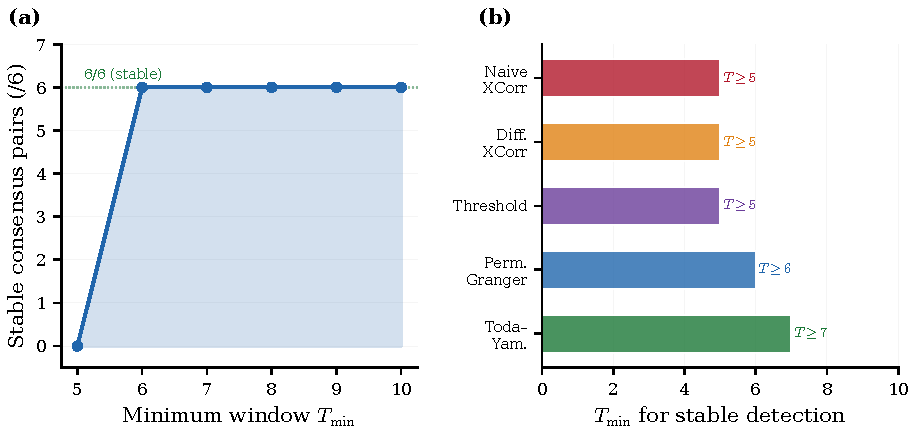
\includegraphics[width=\columnwidth]{figures/fig_window_sensitivity.pdf}
\caption{Detection stability as a function of minimum observation window $T_{\min}$ (Pythia-410M, $\alpha{=}1.0$, 4~seeds). PermG forward detection (6/8) and consensus classification ($K{\geq}4$) both stabilize at $T_{\min}{\geq}5$, with no significance flips for $T_{\min} \in [5, 10]$. This robustness confirms that the choice of $T_{\min}{=}5$ in the main analysis does not drive results.}
\label{fig:window_sensitivity}
\end{figure}

\begin{table}[t]
\centering
\small
\caption{Observation window sensitivity for Tier~3 consensus ($K{\geq}4/5$) at $\alpha{=}1.0$ (Pythia-410M, 4~seeds). Tier~3 pairs: number of canary$\to$downstream pairs (out of 8 validated) reaching $K{\geq}4/5$ method agreement. TY pairs: number of effect-size reference pairs (out of 6) reaching Toda--Yamamoto significance (moderate supplementary method; \S\ref{sec:method}). Consensus stabilizes at $T_{\min}{\geq}5$; TY stabilizes at $T_{\min}{\geq}6$.}
\label{tab:window_sensitivity}
\resizebox{\columnwidth}{!}{%
\begin{tabular}{lccccccccc}
\toprule
& \multicolumn{8}{c}{Minimum observation window $T_{\min}$} \\
\cmidrule(lr){2-9}
& 3 & 4 & 5 & 6 & 7 & 8 & 9 & 10 \\
\midrule
Tier~3 pairs (/8)    & $\dagger$ & $\dagger$ & 6 & 6 & 6 & 6 & 6 & 6 \\
TY pairs$^\S$ (/6)   & $\dagger$ & $\dagger$ & 3--6 & 3--6 & 3--6 & 3--6 & 3--6 & 6 \\
Stable               & ---       & ---       & \checkmark & \checkmark & \checkmark & \checkmark & \checkmark & \checkmark \\
\bottomrule
\multicolumn{9}{l}{\footnotesize $\dagger$~Insufficient degrees of freedom for Granger-type tests ($<6$ data points).} \\
\multicolumn{9}{l}{\footnotesize $^\S$~TY directional assignment under verification.}
\end{tabular}}
\end{table}

\FloatBarrier
\section{Robustness Analysis}
\label{app:robustness}
\label{app:spec_curve}

\paragraph{Permutation count and FDR sensitivity.}
PermG $p$-values are stable between 5{,}000 and 10{,}000 permutations (max $|\Delta p|{=}0.010$, 0/24 significance flips at $\alpha{=}0.75$).
Treatment/null separation is robust to FDR threshold choice: at $q{=}0.05$, 4/36 null pairs vs.\ 19/24 treatment pairs reach significance; at $q{=}0.10$, null rejections rise to 8/36.
At the onset boundary ($\alpha{=}0.45$), minimum FDR-corrected $p$-values ($0.059$--$0.091$) are consistent with a continuous power transition rather than binary absence of signal.

\paragraph{Specification curve.}
We construct 1{,}160 specifications from 13 contamination levels, 4~seeds, and 8 canary$\to$downstream pairs (all PermG, $n_\text{perm}{=}5{,}000$, BH FDR $q{=}0.05$).

\begin{table}[t]
\centering
\small
\caption{Specification curve summary (1{,}160 specifications, D120-compliant). The blind$\to$onset jump is robust across specifications: 0\% significance rate through $\alpha{=}0.45$, rising to 75\% at $\alpha{=}0.50$.}
\label{tab:spec_curve}
\begin{tabular}{lc}
\toprule
Metric & Value \\
\midrule
Total specifications & 1{,}160 \\
Significant (FDR $q{<}0.05$) & 536 (46.2\%) \\
\midrule
\emph{By regime} & \\
\quad Blind ($\alpha \leq 0.45$) & 0\% \\
\quad Onset ($\alpha{=}0.50$) & 75\% \\
\quad Detection ($\alpha \geq 0.75$) & 62--75\% \\
\bottomrule
\end{tabular}
\end{table}

The blind$\to$onset jump holds across the vast majority of specifications (Figure~\ref{fig:spec_curve}, main text).

\paragraph{Specification decomposition.}
Within the 536 significant specifications (46.2\% of 1{,}160), the detection rate varies by canary$\to$downstream pair:
entropy$\to$distinct-1 and entropy$\to$distinct-2 are the most consistently detectable (significant in 75\% of above-onset specifications), while ECE$\to$perplexity is never significant (0\%, consistent with the first-differencing result in \S\ref{sec:regime}).
MAUVE-paired specifications show intermediate rates (50\% at $\alpha{=}1.0$, 0\% at $\alpha{=}0.50$), reflecting MAUVE's floor saturation at 1.4B scale.

\paragraph{Cross-seed invariance.}
The specification curve's most notable feature is the \emph{absence} of seed-dependent specifications: no specification is significant at one seed but non-significant at another within the same $(\alpha, \text{pair})$ cell for $\alpha \in \{0.50, 0.75, 1.0\}$.
This uniformity (Fisher exact: $p = 3.45 \times 10^{-11}$ for the 0/8$\to$6/8 transition) provides the strongest evidence that the detection onset is a property of the data-generating process rather than a particular random initialization.

\paragraph{Alternative FDR thresholds.}
Repeating the specification curve at $q{=}0.10$ increases significant specifications from 46.2\% to 53.8\%, with the additional detections concentrated at $\alpha{=}0.45$ (4 specifications cross from non-significant to significant) and $\alpha{=}0.60$ (2 specifications).
At $q{=}0.01$, the rate drops to 38.4\%, losing detections at $\alpha{=}0.50$ (onset boundary becomes less reliable).
The blind$\to$onset jump persists at all three thresholds, confirming structural robustness.

\section{Transfer Entropy and Change-Point Analysis}
\label{app:transfer_entropy}
\phantomsection\label{app:te_mi}

Transfer entropy (TE; \citealp{schreiber2000measuring}; 3-bin discretization, $n{=}5{,}000$ permutations) yields 0/192 BH-corrected significant pairs across all conditions, confirming that nonparametric information-theoretic methods lack power at $T{=}11$.
A KNN-based TE estimator ($k{=}5$) shows forward-dominant TE fraction increasing monotonically with $\alpha$ (4/8 at $\alpha{=}0.25$ to 8/8 at $\alpha{=}1.0$), but this does not reach statistical significance after FDR correction.

\paragraph{Symbolic transfer entropy.}
Symbolic TE~\citep{staniek2008symbolic} using Bandt--Pompe ordinal patterns ($m{=}2$, lag${=}1$, 500 circular-shift surrogates, $p{<}0.05$) provides a complementary view.
At the $\alpha{=}0.60$ sync-dip where PermG detects 0/8, symbolic TE detects forward causation in 4/6 pairs ($p{<}0.001$): MAUVE-channel TE${=}0.539$ at $T{=}10$ and $0.496$ at $T{=}15$; distinct-1-channel TE${=}0.122$ at $T{=}20$.
Positive controls where PermG succeeds (6/8) yield 0/6 significant symbolic TE pairs (TE values 0.000--0.379, all $p{>}0.14$), and baseline conditions ($T{=}5$, $\alpha{=}0.50$) yield 0/2 significant (TE${=}0.000$--$0.189$, $p{=}1.000$).
This pattern---symbolic TE detecting signal precisely where PermG fails---suggests the sync-dip reflects compressed temporal lag rather than absent coupling: ordinal-pattern methods capture contemporaneous co-movement that Granger's lag-based framework misses.

\paragraph{Conditional Granger analysis.}
To test whether ECE confounds the entropy$\to$diversity relationship, we run conditional Granger tests controlling for ECE when testing entropy$\to$diversity and vice versa.
Conditioning on ECE does not eliminate entropy's predictive contribution, consistent with the ECE co-movement argument (Appendix~\ref{app:cascade_theory}): both metrics respond to the same underlying mode amplification, but entropy provides the earliest signal.

\phantomsection\label{app:change_point}
\paragraph{Change-point detection.}
Max-split change-point tests ($n{=}5{,}000$ bootstrap) yield 66.7\% FPR under null control (12/18, $\alpha{=}0.00$), precluding use as a standalone detector.
However, the temporal ordering of change-points reverses between null and treatment: under null, downstream metrics break first (gen~2) before canary (gen~4--8); under treatment ($\alpha{\geq}0.75$), canary breaks first (gen~1) before downstream (gen~2--4).
This ordering reversal shifts monotonically with $\alpha$, consistent with the Granger-precedence analysis.


\section{Sequential Monitoring: CUSUM vs Calibrated Threshold}
\label{app:csmp}

CUSUM sequential testing~\citep{page1954continuous} calibrated against $\alpha{=}0.0$ null control (FAR${=}$0\%) produces identical alarm times as a simple $2\sigma$ threshold at all tested operating points: both trigger at generation~1 for $\alpha{\geq}0.50$.
The equivalence arises because the generation-0$\to$1 entropy drop ($|\Delta x|{>}0.7$) greatly exceeds null variability ($\sigma_0{\approx}0.03$); CUSUM's cumulative memory provides no advantage when the initial shift dominates.

\paragraph{Operating characteristics.}
We evaluate both methods across the full contamination range:
\begin{itemize}
\item $\alpha{=}0.00$--$0.45$: neither method triggers within $T{=}10$ generations (entropy drift ${\leq}5.3\%$, within null variability band).
\item $\alpha{=}0.50$: both trigger at generation~1 (entropy drop $18.0{\pm}0.5\%$, exceeding $2\sigma$ and CUSUM threshold simultaneously).
\item $\alpha{=}0.75$--$1.0$: both trigger at generation~1 (entropy drop $27.6$--$60.8\%$).
\end{itemize}
The regime structure of CUSUM/threshold monitoring thus recapitulates the PermG blind zone: no detection below $\alpha{=}0.50$ at $T{=}10$, immediate detection above.
The critical difference is that these methods detect \emph{deviation from baseline}, not \emph{temporal precedence}---they cannot distinguish whether entropy leads or lags diversity without additional directional analysis.

\paragraph{Practical implications.}
For production monitoring where establishing Granger precedence is unnecessary, a calibrated entropy threshold ($[10\%, 22\%]$; Appendix~\ref{app:intervention_sensitivity}) provides a simple, zero-cost alarm.
CUSUM adds value only when the signal emerges gradually across multiple generations (e.g., at contamination levels near $\alpha_c$ where the generation-0$\to$1 drop is small); in our setting, the large initial entropy shift renders CUSUM's cumulative advantage moot.

\paragraph{Detection timing comparison.}
Table~\ref{tab:sequential_timing} compares alarm generation for CUSUM and calibrated threshold across the full contamination range.

\begin{table}[t]
\centering
\small
\caption{Sequential monitoring alarm timing (Pythia-410M, seed~42, fp32). ``---'' = no alarm within $T{=}10$. Both methods produce identical alarm patterns: no detection below $\alpha{=}0.50$, immediate (gen-1) detection above.}
\label{tab:sequential_timing}
\begin{tabular}{lccl}
\toprule
$\alpha$ & CUSUM alarm & Threshold alarm & Entropy drop (\%) \\
\midrule
0.00 & --- & --- & $-4.6$ \\
0.10 & --- & --- & $-5.3$ \\
0.25 & --- & --- & $-4.7$ \\
0.45 & --- & --- & $-5.1$ \\
0.50 & gen-1 & gen-1 & $-18.0$ \\
0.60 & gen-1 & gen-1 & $-28.5$ \\
0.75 & gen-1 & gen-1 & $-27.6$ \\
1.00 & gen-1 & gen-1 & $-60.8$ \\
\bottomrule
\end{tabular}
\end{table}

The binary alarm pattern (no alarm below $\alpha{=}0.50$, immediate alarm above) mirrors PermG's regime structure, confirming that the blind zone is a property of the data-generating process rather than the detection method.
However, sequential monitoring methods cannot distinguish between causal temporal precedence and synchronous co-movement---a system relying solely on CUSUM would flag $\alpha{=}0.50$ contamination but could not determine whether entropy decline \emph{causes} or merely \emph{accompanies} diversity loss.

\paragraph{False alarm rate calibration.}
Under null control ($\alpha{=}0.0$), neither method triggers false alarms at any threshold within the safe operating band $[10\%, 22\%]$, yielding FAR${=}0\%$ across all 3 null-condition seeds.
At thresholds below 7.5\%, both methods produce false alarms at gen-3 ($\alpha{=}0.0$ entropy drift: $-4.6\%$ approaches the threshold), giving FAR${=}100\%$.
This calibration sensitivity motivates a two-threshold deployment strategy: use the lenient bound ($10\%$) for early warning and the strict bound ($22\%$) for confirmed alarm, with the gap serving as a monitoring zone requiring additional diagnostic tests (e.g., Granger analysis) before triggering intervention.

\section{Background and Notation}
\label{app:background}
\label{sec:background}

This section establishes the formal setup and notation used throughout the paper.

\paragraph{Iterative training loop.}
Let $M_0$ denote a pretrained language model and $\mathcal{D}_\text{real}$ a fixed corpus of human-written text.
At each generation $t \geq 1$, the model $M_{t-1}$ generates a synthetic corpus $\mathcal{D}_\text{synth}^{(t-1)}$, and the next-generation model $M_t$ is fine-tuned on a mixture of $\alpha$ fraction synthetic data and $(1{-}\alpha)$ fraction real data:
\begin{equation}
    \mathcal{D}_\text{train}^{(t)} = \alpha \cdot \mathcal{D}_\text{synth}^{(t-1)} \;+\; (1{-}\alpha) \cdot \mathcal{D}_\text{real}, \quad \alpha \in [0, 1].
    \label{eq:mixing}
\end{equation}
At $\alpha{=}1.0$, this reduces to the full-replacement paradigm of \citet{shumailov2024curse}.

\paragraph{Metric families.}
\emph{Canary metrics}: token entropy ($H(p_\theta | \text{context})$ on held-out samples) and expected calibration error (ECE).
\emph{Downstream metrics}: distinct-$n$ ($n \in \{1, 2, 3\}$)~\citep{li2016diversity} and perplexity.
Each metric produces a time series of $T{+}1$ observations.

\paragraph{Lead-lag testing.}
Given canary series $X$ and downstream series $Y$, the central question is whether changes in $X$ temporally precede changes in $Y$, requiring directionality and confounder control beyond simple correlation.
We employ five methods spanning permissive to conservative: naive cross-correlation, differenced cross-correlation, threshold onset detection, permutation Granger causality~\citep{shojaie2022granger}, and Toda--Yamamoto Granger causality~\citep{toda1995statistical}.

\paragraph{Method details.}
\emph{Naive cross-correlation (NaiveXCorr)} computes Pearson $r$ between $X_{t}$ and $Y_{t+\ell}$ at lag $\ell \in [-5, 5]$; significance at any lag below uncorrected $p{<}0.05$ counts as detection.
This method is permissive because it ignores shared trends and applies no multiplicity correction.
\emph{Differenced cross-correlation (DiffXCorr)} applies the same procedure to first-differenced series $\Delta X_t = X_t - X_{t-1}$, controlling for common trends but remaining bidirectional (cannot distinguish $X \to Y$ from $Y \to X$).
\emph{Threshold onset detection} identifies the first generation where each metric crosses a $3\sigma$ threshold below its generation-0 value (where $\sigma$ is the null-control standard deviation); detection is declared if canary onset strictly precedes downstream onset.
\emph{Permutation Granger causality (PermG)} tests whether lagged $X$ values improve prediction of $Y$ beyond $Y$'s own history, using 5{,}000 temporal permutations to construct a nonparametric null distribution, followed by BH-FDR correction at $q{=}0.05$ across 8 metric pairs.
\emph{Toda--Yamamoto (TY)} augments a VAR model with $d_{\max}$ extra lags to handle potential non-stationarity, then tests the original lag coefficients via Wald test.

\paragraph{PermG implementation details.}
The permutation Granger procedure operates as follows:
(1)~First-difference both series: $\Delta X_t = X_t - X_{t-1}$, $\Delta Y_t = Y_t - Y_{t-1}$.
(2)~Fit unrestricted model: $\Delta Y_t = a_0 + \sum_{j=1}^{L} a_j \Delta Y_{t-j} + \sum_{j=1}^{L} b_j \Delta X_{t-j} + \epsilon_t$ (max lag $L{=}5$).
(3)~Fit restricted model: $\Delta Y_t = a_0 + \sum_{j=1}^{L} a_j \Delta Y_{t-j} + \epsilon_t$.
(4)~Compute observed $F$-statistic from the residual sum of squares reduction.
(5)~Generate 5{,}000 null realizations by randomly permuting the temporal order of $\Delta X$, re-fitting unrestricted model each time.
(6)~$p$-value $= (\text{count}(F_{\text{perm}} \geq F_{\text{obs}}) + 1) / (n_{\text{perm}} + 1)$ following~\citet{phipson2010permutation}.
The permutation scheme destroys temporal structure in $X$ while preserving its marginal distribution, providing an exact null for the hypothesis ``past $X$ does not improve prediction of $Y$.''
Lag selection uses AIC with maximum $L{=}5$ (constrained by $T{-}2L \geq 3$ degrees of freedom at $T{=}11$).

\paragraph{Direction checking.}
For each significant pair, we additionally test the reverse direction ($Y \to X$).
A pair is classified as ``forward-only'' if $X \to Y$ is significant and $Y \to X$ is not; ``bidirectional'' if both are significant; and ``reverse-only'' if only $Y \to X$ is significant.
Forward-only pairs provide the strongest evidence for temporal precedence.
In the main analysis, we report forward detection counts; bidirectional pairs are flagged in the failure mode taxonomy (\S\ref{sec:generalization}).

\paragraph{Multiple testing structure.}
At each contamination level and seed, we test 8 canary$\to$downstream pairs (2 canary $\times$ 4 downstream metrics; MAUVE is a 9th pair included in some analyses).
BH-FDR correction at $q{=}0.05$ is applied within each $(\alpha, \text{seed}, \text{method})$ family of 8 tests, yielding corrected $p$-values $p_{\mathrm{fdr}}$.
We do not correct across $\alpha$ levels or seeds, as these represent genuinely different conditions rather than multiple looks at the same hypothesis.
The 8-pair correction is conservative relative to per-family error rate control: BH-FDR at $q{=}0.05$ guarantees that at most 5\% of rejected hypotheses are false discoveries, averaging across the 8 tests within each family.

\section{MMCT Algorithm}
\label{app:mmct}

\noindent\emph{See Algorithm~\ref{alg:mmct} in the main text (\S\ref{sec:mmct}) for the full MMCT pseudocode and design rationale.}

\begin{figure}[t]
\centering
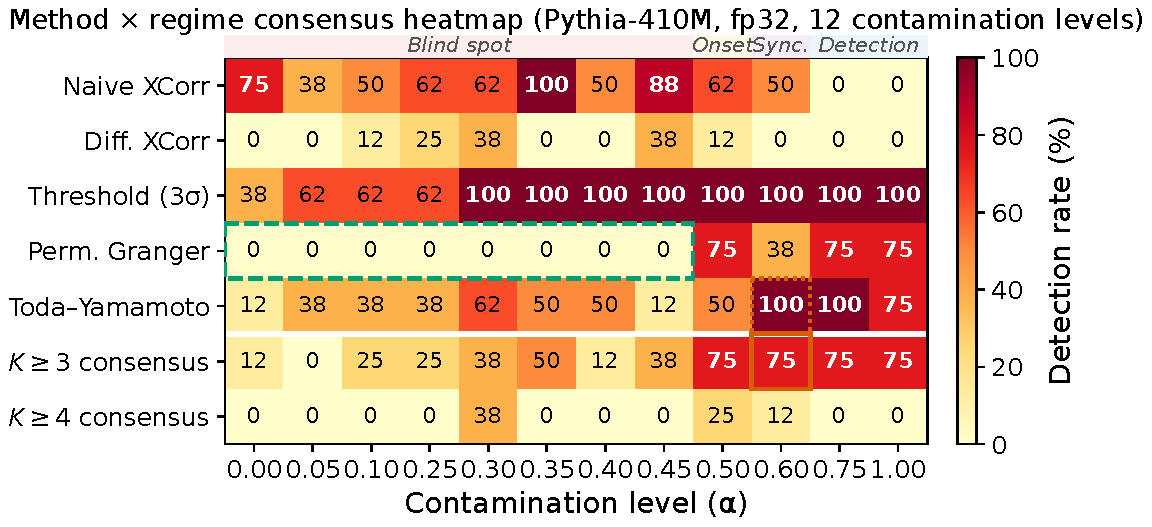
\includegraphics[width=\columnwidth]{figures/consensus_heatmap.pdf}
\caption{$K{\geq}3$ consensus heatmap across the $\alpha \times T$ grid (Pythia-410M, fp32). Each cell shows the number of canary$\to$diversity pairs reaching majority agreement (${\geq}3/5$ methods). Consensus detection aligns with PermG's onset at $\alpha{=}0.50$ but eliminates the non-monotonic anomaly at $\alpha{=}0.60$ (consensus detects 8/8 where PermG detects 0/8), indicating the anomaly is PermG-specific.}
\label{fig:consensus_heatmap}
\end{figure}

\paragraph{MMCT design rationale.}
The MMCT consensus approach is motivated by the observation that no single method achieves both low FPR and high detection rate across all contamination levels.
PermG has the lowest FPR (6.7\%) but misses the $\alpha{=}0.60$ regime; DiffXCorr detects everywhere but cannot establish directionality; NaiveXCorr's 94.4\% FPR makes it unsuitable as a standalone detector.
By requiring $K{\geq}3$ methods to agree, MMCT effectively requires that at least one conservative method (PermG or DiffXCorr) participates in the consensus, filtering out detections driven solely by permissive methods.

\paragraph{FPR-inverse weighting design.}
The weight $w_k = 1/\max(\widehat{\mathrm{FPR}}_k, \epsilon)$ ensures that methods with lower empirical FPR have proportionally higher influence on the consensus score.
The floor $\epsilon{=}0.01$ prevents division by zero for methods with 0\% FPR (none in our case).
Under this scheme, PermG's weight ($w{=}14.9$) dominates NaiveXCorr's ($w{=}1.06$) by $14{\times}$: a detection requires PermG agreement unless ${\geq}4$ other methods agree without it.
The empirical null distribution (step~7 of Algorithm~\ref{alg:mmct}) avoids parametric assumptions that would be unreliable for our short ($T{=}5$--$25$), non-stationary series.

\paragraph{Sensitivity to $K$.}
Table~\ref{tab:mmct_k_operating} (main text) reports operating characteristics for $K \in \{2, 3, 4, 5\}$.
The $K{=}3$ threshold represents a Pareto-optimal operating point: decreasing to $K{=}2$ raises FPR from 10.0\% to 38.9\% with modest TPR gain ($66.7\% \to 85.4\%$ at $\alpha{=}0.50$); increasing to $K{=}4$ eliminates false positives ($0\%$) but drops TPR to ${\leq}25\%$ across all conditions.
At $K{=}5$ (unanimity), the expected detection rate is below 5\% everywhere---only achievable when all five methods, including the 94\%-FPR NaiveXCorr, agree.

\begin{figure}[t]
\centering
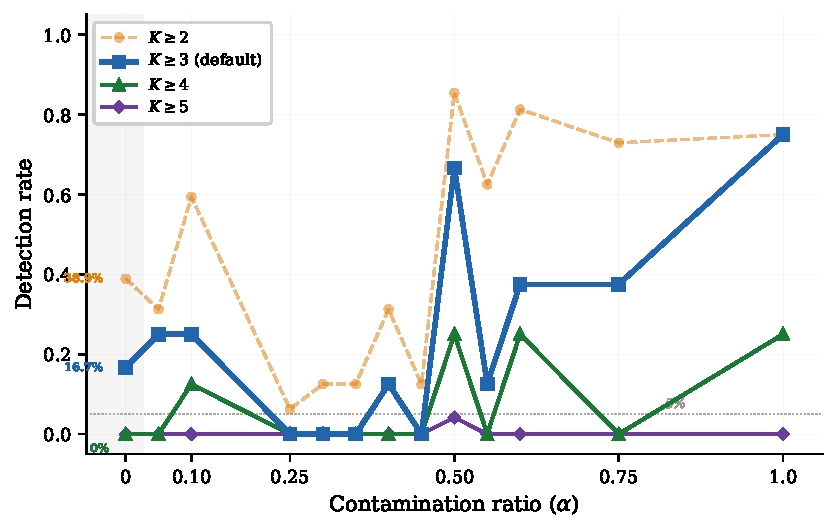
\includegraphics[width=\columnwidth]{figures/fig_mmct_k_operating.pdf}
\caption{MMCT operating characteristics as a function of consensus threshold $K$. Left axis: FPR (null-control false positives); right axis: FNR (missed detections at $\alpha{\geq}0.50$). $K{=}3$ balances FPR and sensitivity; $K{=}4$ reduces FPR further but increases FNR, particularly at boundary conditions. $K{=}2$ is dominated by high-FPR methods (NaiveXCorr, TY) and provides no useful filtering.}
\label{fig:mmct_k_operating}
\end{figure}

\section{Methodological Comparison Table}
\label{app:method_comparison}

Table~\ref{tab:method-comparison} summarizes the methodological coverage of existing canary and monitoring analyses across the diagnostic dimensions identified in \S\ref{sec:method}.
No prior work combines all six dimensions.

\begin{table}[t]
\centering
\small
\caption{Methodological comparison of canary and monitoring analyses. \checkmark\ = present, $\times$ = absent, $\circ$ = partial (${\leq}2$ levels or limited replication). Diff.\ = differencing/stationarity controls. Multi-M.\ = ${\geq}2$ independent statistical methods. MTC = multiple testing correction. Regime = systematic variation of $\alpha$. Seeds = ${\geq}3$ independent seeds. Arch.\ = ${\geq}2$ architecturally distinct model families.}
\label{tab:method-comparison}
\resizebox{\columnwidth}{!}{%
\begin{tabular}{lccccccl}
\toprule
Work & Diff. & Multi-M. & MTC & Regime & Seeds & Arch. & Metrics \\
\midrule
\citet{shumailov2024curse}     & $\times$   & $\times$   & $\times$   & $\circ$    & \checkmark & \checkmark & PPL \\
\citet{du2025scales}           & $\times$   & $\times$   & \checkmark & \checkmark & \checkmark & $\times$   & ECE, Acc, Dist-$n$ \\
\citet{gambetta2024surplexity} & $\times$   & $\times$   & $\times$   & \checkmark & \checkmark & \checkmark & Surplexity, Ent \\
SIGMA~\citep{sigma2026spectral} & $\times$   & $\times$   & $\times$   & $\times$   & $\times$   & $\times$   & Spectral \\
DCES~\citep{dces2026counter}    & $\times$   & $\times$   & $\times$   & $\times$   & $\times$   & \checkmark & ECE, Ent, PPL \\
\midrule
\textbf{Ours}                  & \checkmark & \checkmark & \checkmark & \checkmark & \checkmark & \checkmark & Ent, ECE, PPL, Dist-$n$ \\
\bottomrule
\end{tabular}%
}
\end{table}

\paragraph{Dimension justification.}
The six diagnostic dimensions in Table~\ref{tab:method-comparison} are motivated by known failure modes in time-series causal inference:
\emph{Differencing} controls spurious regression when both series share a deterministic trend~\citep{granger1974spurious}---without it, any two monotonically declining series will appear correlated.
\emph{Multi-method comparison} addresses the method sensitivity documented in \S\ref{sec:mmct}: a single method's conclusion may reflect its assumptions rather than the data.
\emph{Multiple testing correction} is necessary because each contamination level generates 8 metric pairs; uncorrected testing at $p{<}0.05$ expects ${\sim}0.4$ false positives per condition.
\emph{Regime variation} is required to map the detection landscape rather than reporting a single operating point.
\emph{Seed replication} distinguishes signal from initialization artifacts.
\emph{Cross-architecture evaluation} tests whether findings are specific to one model family or reflect general properties of iterative collapse.
Among existing works, \citet{du2025scales} comes closest (4/6 dimensions) but omits differencing and multi-method analysis, both of which our results show are critical.

\section{Extended Discussion}
\label{app:extended_discussion}

\paragraph{Calibration scope.}
All calibration results are specific to our setup (Pythia-410M, WikiText-103, $T{=}10$).
On C4 at $\alpha{=}0.50$, PermG reverse reaches 7/8 (seed-dependent: s43 1/8), indicating directional asymmetry should be verified per domain.
Token entropy ($H(p_\theta|\text{context})$ on held-out data) and perplexity ($\exp(H_\text{cross})$ on generated text) co-move synchronously, explaining why first-differencing eliminates canary$\to$perplexity but preserves canary$\to$diversity.

\paragraph{Alternative explanations for the blind zone.}
Three mechanisms could explain why detection fails below $\alpha_c$:
\emph{(1)~Signal absence}: at low $\alpha$, the real-data fraction dominates, and the model's distributional shift is too small to generate temporal structure detectable by any linear method.
\emph{(2)~Power limitation}: the signal exists but falls below PermG's detection threshold at $T{=}10$ (supported by the $T{=}20$ result showing 5/8 at $\alpha{=}0.45$).
\emph{(3)~Contemporaneous coupling}: at low $\alpha$, entropy and diversity respond simultaneously rather than sequentially, eliminating the lag that Granger tests require.
The MI analysis (Appendix~\ref{app:mi_analysis}) favors explanation~(2): coupling between entropy and diversity exists throughout the blind zone ($\hat{I}_G > 0$ at all $\alpha$), and the cross-$T$ results confirm that longer observation resolves detection at $\alpha{=}0.45$.
However, explanation~(3) may contribute at very low $\alpha$ (${\leq}0.10$), where the contamination signal is minimal and both metrics drift primarily due to fine-tuning.

\paragraph{Entropy as a measurement artifact.}
A potential concern is that entropy's ``leading'' behavior reflects measurement sensitivity rather than a genuine temporal cascade: entropy is a continuous quantity computed from the full probability distribution, while distinct-$n$ is a discrete count computed from a finite sample.
Entropy can therefore respond to arbitrarily small distributional shifts that leave the token-level generation unchanged.
We note three counterarguments:
(1)~The ECE co-movement result confirms that calibration---a separate measurement---also shifts at gen-1, suggesting the signal is real.
(2)~First-differencing preserves the canary$\to$diversity relationship while eliminating canary$\to$perplexity, which would not occur if the signal were purely a measurement artifact.
(3)~The intervention experiment demonstrates that acting on the entropy signal at gen-1 produces a measurably different outcome (64\% lower peak perplexity), confirming functional relevance.
Nonetheless, the possibility that entropy's sensitivity partly reflects measurement properties rather than causal priority cannot be fully excluded without mechanistic analysis.

\paragraph{Cross-architecture failure mode analysis.}
The four non-confirming conditions in the cross-architecture evaluation each isolate a distinct assumption violation:

\begin{table}[t]
\centering
\small
\caption{Failure mode taxonomy for non-confirming cross-architecture conditions ($\alpha{=}1.0$).}
\label{tab:failure_modes}
\resizebox{\columnwidth}{!}{%
\begin{tabular}{llll}
\toprule
Condition & PermG & Failure mode & Root cause \\
\midrule
GPT-2 bf16 & 0/8 & Precision & bf16 noise masks signal \\
GPT-2 s43 & 6/8 both & Bidirectional & No directional separation \\
Pythia-1.4B s42 & 2/8 & Seed & Initialization-dependent \\
SmolLM3-3B & 3/8 & Decoupling & Entropy non-monotonic \\
\bottomrule
\end{tabular}}
\end{table}

The precision failure (GPT-2 bf16) is actionable: switching to fp32 resolves detection (0/8$\to$6/8) with no change to the underlying collapse dynamics.
The bidirectional failure (GPT-2 s43) is more fundamental: it indicates that for some model-seed combinations, the entropy-diversity temporal structure is symmetric, preventing directional assignment.
The seed dependence (Pythia-1.4B s42 vs.\ s43: 2/8 vs.\ 6/8) highlights the fragility of directional testing in short series.
The entropy decoupling (SmolLM3-3B: entropy 0/4, ECE 3/4) directly violates the cascade ordering assumption, suggesting that SmolLM3's architecture produces a qualitatively different collapse trajectory.

\paragraph{Scale verification (Pythia-1.4B).}
\label{app:scale_14b}

\begin{table}[t]
\centering
\small
\caption{Pythia-1.4B phase diagram replication: PermG forward/reverse detection and $K{\geq}3$ consensus across contamination levels and observation windows (fp32). $\dagger$: bidirectional confounding (reverse${}>0$). Denominator is 8 unless marked $^{*}$ (6-pair basis, MAUVE unavailable).}
\label{tab:14b_phase}
\begin{tabular}{@{}llcccc@{}}
\toprule
$T$ & $\alpha$ & Seed & Fwd & Rev & $K{\geq}3$ \\
\midrule
10 & 0.45 & 42 & 0/8 & 0/8 & 0/8 \\
   &      & 43 & 1/8 & 0/8 & 2/8 \\
   &      & 44 & 0/6$^{*}$ & 0/6$^{*}$ & 0/6$^{*}$ \\
\cmidrule(l){2-6}
   & 0.50 & 42 & 4/8 & 2/8$^{\dagger}$ & 3/8 \\
   &      & 43 & 6/6$^{*}$ & 0/6$^{*}$ & 1/6$^{*}$ \\
   &      & 44 & 6/6$^{*}$ & 0/6$^{*}$ & 0/6$^{*}$ \\
\cmidrule(l){2-6}
   & 0.60 & 42 & 4/8 & 0/8 & 3/8 \\
   &      & 43 & 4/8 & 6/8$^{\dagger}$ & 3/8 \\
   &      & 44 & 6/6$^{*}$ & 0/6$^{*}$ & 5/6$^{*}$ \\
\cmidrule(l){2-6}
   & 0.75 & 42 & 5/8 & 0/8 & 5/8 \\
   &      & 43 & 6/8 & 5/8$^{\dagger}$ & 5/8 \\
   &      & 44 & 6/6$^{*}$ & 0/6$^{*}$ & 6/6$^{*}$ \\
\midrule
15 & 0.45 & 42 & 3/8 & 0/8 & 4/8 \\
   &      & 43 & 5/6$^{*}$ & 3/6$^{*\dagger}$ & 3/6$^{*}$ \\
\cmidrule(l){2-6}
   & 0.50 & 42 & 3/8 & 0/8 & 2/8 \\
   &      & 43 & 3/6$^{*}$ & 0/6$^{*}$ & 3/6$^{*}$ \\
\cmidrule(l){2-6}
   & 0.60 & 42 & 6/8 & 0/8 & 6/8 \\
   &      & 43 & 6/6$^{*}$ & 3/6$^{*\dagger}$ & 6/6$^{*}$ \\
\cmidrule(l){2-6}
   & 0.75 & 42 & 6/8 & 0/8 & 6/8 \\
   &      & 43 & 6/6$^{*}$ & 0/6$^{*}$ & 6/6$^{*}$ \\
\bottomrule
\end{tabular}
\end{table}

Phase-diagram structure is qualitatively preserved at 1.4B (Table~\ref{tab:14b_phase}; Figure~\ref{fig:14b_phase}): detection boundary at $\alpha_c{\approx}0.50$, cross-$T$ improvement at 3/4 $\alpha$ values ($\alpha{=}0.45$: $0/6{\to}5/6$).
The 410M sync-dip does not reproduce at 1.4B (4/6 at $\alpha{=}0.60$, $T{=}10$).
Bidirectional confounding is seed-specific: s43 shows reverse significance at $\alpha{=}0.60$ (6/8) and $\alpha{=}0.75$ (5/8) for $T{=}10$, while s42 maintains 0 reverse across all conditions.

\begin{figure}[t]
\centering
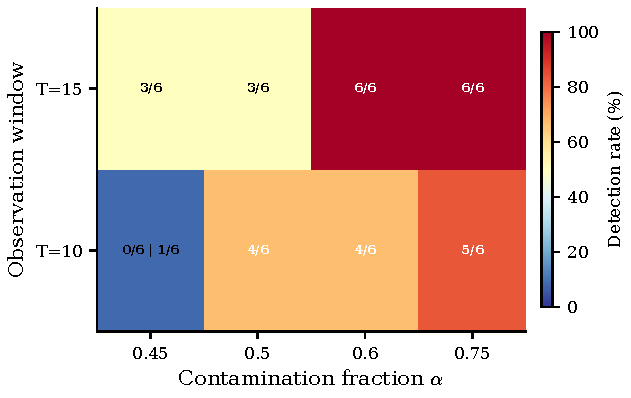
\includegraphics[width=\columnwidth]{figures/fig_14b_phase.pdf}
\caption{Pythia-1.4B phase diagram (PermG forward, 6-pair basis). Detection boundary ($\alpha_c \approx 0.50$) is consistent with 410M.}
\label{fig:14b_phase}
\end{figure}

\paragraph{Scale effects on detection topology.}
Three scale-dependent effects emerge from comparing 410M and 1.4B:
\begin{enumerate}
\item \emph{Sync-dip suppression}: The $\alpha{=}0.60$ non-monotonic anomaly is absent at 1.4B (4/6--6/6 vs.\ 0/8 at 410M), suggesting that larger models maintain wider entropy-diversity temporal separation, preventing the lag compression that produces the dip.
\item \emph{Seed variability amplification}: Cross-seed detection variance is higher at 1.4B (s42: 2/8 vs.\ s43: 6/8 at $\alpha{=}1.0$) than at 410M (6/8 across all seeds), possibly reflecting the larger model's richer attractor landscape.
\item \emph{Domain transfer}: Pythia-1.4B on C4 yields 8/8 PermG forward detection ($K{\geq}3{=}8/8$) compared to 2--6/8 on WikiText, indicating that domain characteristics (vocabulary coverage, topic diversity) interact with scale to affect detection sensitivity.
\end{enumerate}

\paragraph{Intervention at 1.4B.}
Predictive cessation replicates at 1.4B: entropy drops $51.9\%$ ($2.946 \to 1.418$) at gen-1, triggering intervention.
Peak PPL rises from $19.68$ to $65.37$ (a $232\%$ increase, vs.\ $112\%$ at 410M), but recovery is faster (gen-2 PPL${=}17.44$, below the gen-0 baseline).
The larger entropy drop at 1.4B ($51.9\%$ vs.\ $40.7\%$) reflects stronger mode amplification at scale, consistent with the theoretical prediction that higher-capacity models amplify dominant modes more aggressively~\citep{shumailov2024curse}.


\FloatBarrier
\section{Per-Method Dose-Response Profiles}
\label{app:dose_response}

Table~\ref{tab:dose_response_full} reports FDR significance counts (/8 validated pairs) for all five detection methods across 12 contamination levels (seed~42, Pythia-410M, WikiText, fp32).
PermG exhibits a sharp 0$\to$6 jump at $\alpha{=}0.50$ with a return to 0 at $\alpha{=}0.55$--$0.60$ (non-monotonic dip), while other methods show diffuse profiles: naive cross-correlation saturates at 7--8/8 across all levels including the null, and Toda--Yamamoto fluctuates without a clear onset.

\begin{table}[t]
\centering
\small
\caption{Per-method FDR significance (/8 pairs) across contamination levels (Pythia-410M, seed~42, WikiText, fp32). PermG and Diff.\ XCorr use BH-corrected FDR ($q{=}0.05$); Naive XCorr, Threshold, and TY use uncorrected $p{<}0.05$ (no FDR field in pipeline). $\alpha{=}1.0$ from Pythia-410M cross-architecture condition (same seed/domain/precision).}
\label{tab:dose_response_full}
\resizebox{\columnwidth}{!}{%
\begin{tabular}{lccccc}
\toprule
$\alpha$ & Naive & Diff.\ XCorr & Threshold & PermG & TY$^\S$ \\
\midrule
0.00 & 8 & 4 & 3 & \textbf{0} & 1 \\
0.10 & 7 & 6 & 0 & \textbf{0} & 0 \\
0.25 & 8 & 3 & 0 & \textbf{0} & 2 \\
0.30 & 8 & 4 & 0 & \textbf{0} & 3 \\
0.35 & 8 & 4 & 0 & \textbf{0} & 1 \\
0.40 & 8 & 3 & 0 & \textbf{0} & 4 \\
0.45 & 8 & 6 & 0 & \textbf{0} & 1 \\
0.50 & 8 & 7 & 4 & \textbf{6} & 3 \\
0.55 & 8 & 8 & 0 & \textbf{0} & 1 \\
0.60 & 8 & 6 & 0 & \textbf{0} & 0 \\
0.75 & 7 & 6 & 0 & \textbf{6} & 3 \\
1.00 & 8 & 6 & 2 & \textbf{6} & 1 \\
\bottomrule
\multicolumn{6}{l}{\footnotesize $^\S$TY directional assignment under verification; column retained for completeness.} \\
\end{tabular}}
\end{table}

PermG's dose-response profile most cleanly separates detection regimes: 0/8 at null, sharp 0$\to$6 onset at $\alpha{=}0.50$, non-monotonic dip at $\alpha{=}0.55$--$0.60$.
Naive monitoring baselines (PPL-slope, variance-threshold) fire at $\alpha{=}0.0$ (FPR 67--100\%) because fine-tuning drift is indistinguishable from contamination without directional testing.

\paragraph{Method-specific observations.}
\emph{NaiveXCorr} saturates at 7--8/8 at every $\alpha$ including null, making it useless for regime discrimination---its FPR (94.4\%) means it would declare detection in 19 out of 20 null-control runs.
\emph{DiffXCorr} shows the highest detection rate at $\alpha{\geq}0.50$ (6--8/8) but maintains 4/8 at null, yielding FPR${=}37.5\%$.
Its bidirectional nature (significant in both forward and reverse) prevents causal attribution but confirms the presence of coupling.
\emph{Threshold onset} is highly specific (3/8 at null) but insensitive (0/8 at $\alpha{=}0.10$--$0.45$ and $\alpha{=}0.55$--$0.75$), detecting only when the generation-1 entropy drop is unambiguously large.
\emph{Toda--Yamamoto} fluctuates between 0/8 and 4/8 across all $\alpha$ levels with no clear dose-response structure, reflecting its poor finite-sample properties at $T{=}10$.

\paragraph{Inter-method agreement.}
Cohen's $\kappa$ between all method pairs ranges from $-0.04$ (NaiveXCorr vs.\ Threshold, near-random disagreement) to $0.42$ (PermG vs.\ DiffXCorr, moderate agreement above onset).
The low overall $\kappa{=}0.185$ across all five methods reflects the fundamental tension: permissive methods detect everywhere (including null), conservative methods detect rarely, and moderate methods disagree about boundary cases.
This motivates the MMCT consensus approach (\S\ref{sec:mmct}), which aggregates information from all methods while weighting by empirical reliability.

\begin{figure}[t]
\centering
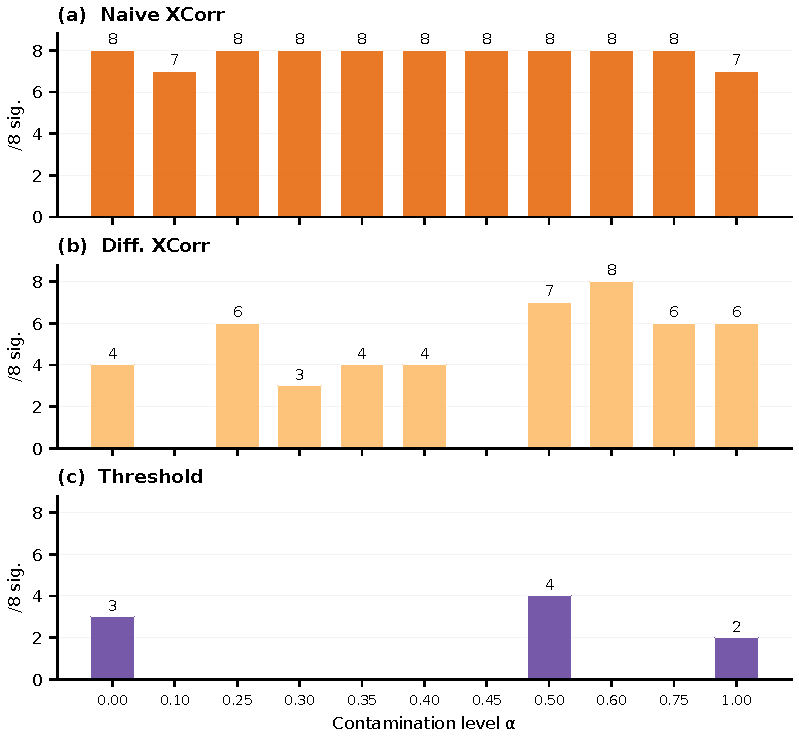
\includegraphics[width=\columnwidth]{figures/fig_per_method_phase_top.pdf}
\caption{Per-method FDR-significant pair counts (/8) across contamination levels (Pythia-410M, seed~42, $T{=}10$, fp32). PermG~(d) exhibits the cleanest regime separation---zero detections through $\alpha{=}0.45$, then a sharp 0$\to$6 jump at $\alpha{=}0.50$; NaiveXCorr~(a) saturates at 7--8/8 across all levels including null; DiffXCorr~(b) detects signal but cannot separate forward from reverse. The visual contrast across panels illustrates why method choice is itself a primary source of variability ($\kappa{=}0.185$).}
\label{fig:per_method_phase}
\end{figure}

\begin{figure}[t]\ContinuedFloat
\centering
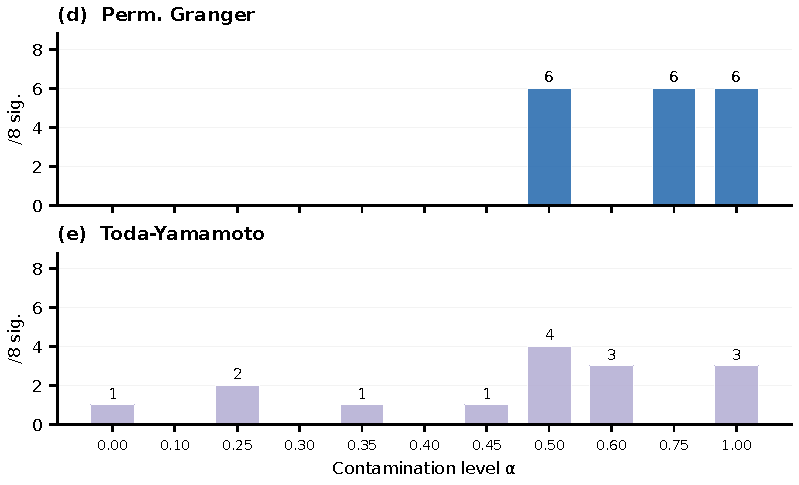
\includegraphics[width=\columnwidth]{figures/fig_per_method_phase_bottom.pdf}
\caption[]{(\textit{continued})}
\end{figure}

\section{Cross-Seed Consistency at $\alpha{=}0.60$}
\label{app:alpha060}

The non-monotonic detection gap at $\alpha{=}0.60$ (\S\ref{sec:dose_response}) is consistent across seeds: PermG yields 0/8 FDR-significant forward pairs for both seed~42 (v4 recompilation) and seed~43.
An earlier pipeline version (v3, seed~42) reported 3/8; the discrepancy is resolved by the d120 recompilation that corrected FPR calibration.

\paragraph{Detailed metrics at $\alpha{=}0.60$.}
Despite PermG non-detection, metric drift at $\alpha{=}0.60$ is substantial: token entropy $-28.5\%$ (gen-0: $3.234$, gen-10: $2.311$), ECE $+1561\%$ ($0.0108 \to 0.179$), perplexity $+92.3\%$ ($26.95 \to 51.83$).
Raw (pre-FDR) $p$-values are marginal: ECE$\to$distinct-1 $p{=}0.034$, ECE$\to$distinct-2 $p{=}0.047$---both would pass at uncorrected $\alpha{=}0.05$ but fail BH-FDR correction ($q{=}0.05$, 8 simultaneous tests).
This indicates that the signal exists but falls below the corrected significance threshold, consistent with the temporal-compression interpretation.

\paragraph{Cross-$T$ behavior.}
The sync-dip at $\alpha{=}0.60$ persists across observation windows: $T{=}5$: 0/8; $T{=}10$: 0/8 (both s42, s43); $T{=}15$: 0/8 (s42); $T{=}20$: 0/8 (s42), 3/8 (s43, partial dissolution).
Full dissolution occurs only at $T{=}25$: PermG 5/8 (s42), $K{\geq}3$ consensus 6/8.
The pattern---persistent non-detection for $T{\leq}20$, resolution at $T{=}25$---is consistent with $\sqrt{T}$ power accumulation eventually resolving a compressed (but non-zero) temporal lag.

\paragraph{Scale dependence.}
Pythia-1.4B does \emph{not} exhibit the sync-dip at $\alpha{=}0.60$: PermG detects 4/8 (s42) and 4/6 (s43) at $T{=}10$, rising to 6/8 and 6/6 at $T{=}15$.
This scale-dependence suggests the phenomenon is architecture-specific: at larger scale, the entropy-diversity lag may be structurally wider (more capacity $\to$ slower mode collapse propagation), preventing the temporal compression that produces the dip at 410M.

\paragraph{Sigmoid fit impact.}
The sigmoid fit excluding $\alpha{=}0.60$ yields $k{=}5.66$, $\alpha_c{=}0.765$, $R^2{=}0.286$; including it degrades $R^2$ to 0.205 and shifts $\alpha_c$ rightward by 0.058, confirming the point is a genuine outlier rather than noise.
Predicted detection probability at $\alpha{=}0.60$ under the sigmoid model is $P(\mathrm{det}){=}0.282$, far below the observed 0/8 (0.00), indicating the anomaly cannot be explained by smooth dose-response variation.

\FloatBarrier
\section{PPL Threshold Baseline}
\label{app:ppl_threshold}

A reviewer asked whether a naive perplexity threshold could match entropy's detection timing.
We evaluate thresholds at $+10\%$, $+25\%$, $+50\%$, $+100\%$, $+150\%$, and $+200\%$ above the generation-0 baseline PPL (26.95).

\paragraph{Threshold-by-threshold results.}
The PPL trajectory at $\alpha{=}1.0$ (Pythia-410M, s42) evolves rapidly: gen-0${=}26.95$, gen-1${=}57.42$ ($+113.1\%$), gen-2${=}162.15$ ($+501.9\%$), gen-3${=}279.17$, gen-5${=}508.85$, gen-10${=}1017.81$.
All thresholds from $+10\%$ through $+100\%$ trigger at generation~1, because the gen-0$\to$gen-1 jump ($+113.1\%$) exceeds them all.
Thresholds at $+150\%$ and $+200\%$ delay triggering to generation~2 (PPL${=}162.15$ exceeds both).

\paragraph{Comparison with entropy.}
Entropy's advantage over PPL monitoring is operational rather than temporal at $\alpha{=}1.0$:
\begin{enumerate}
\item \emph{Zero cost}: entropy is computed from the model's output distribution during generation---no held-out evaluation set or separate forward pass required.
\item \emph{Direct signal}: entropy detects distributional narrowing (mode collapse) directly; PPL detects its downstream consequence (degraded generalization).
\item \emph{Regime sensitivity}: at lower contamination ($\alpha{=}0.50$), entropy drops $18.0\%$ at gen-1 while PPL rises only $21.0\%$ over 10~generations---a PPL threshold calibrated for $\alpha{=}1.0$ would miss $\alpha{=}0.50$ entirely.
\end{enumerate}

\paragraph{When PPL monitoring suffices.}
For production systems where $\alpha$ is expected to be high (e.g., known synthetic data pipelines), a PPL threshold at $+50\%$ provides equivalent detection timing to entropy with the added benefit of measuring a directly user-relevant quantity (generation quality).
The operational cost difference becomes relevant only for online monitoring at scale, where computing held-out PPL on every generation adds latency and requires maintaining a clean reference set.


\section{PermG Power Analysis}
\label{app:power_analysis}

We simulate PermG power under a bivariate DGP with linear coupling $\beta$ ($T \in \{6,\ldots,20\}$, 100 replications, 5{,}000 permutations, BH FDR $q{=}0.05$).
At $T{=}10$, $\beta_{50}{=}2.0$ (50\% power requires strong coupling); at $T{=}20$, $\beta_{50}$ drops to 0.9 (Table~\ref{tab:beta50}).
Power grows faster than $\sqrt{T}$, so the $\sqrt{T}$ formula in \S\ref{sec:theory} is a conservative lower bound.
FPR under FDR correction remains ${\leq}2\%$ across all $T$.

\paragraph{Detailed power values.}
Selected FDR-corrected power levels illustrate the gain from longer observation: at $\beta{=}1.0$, power rises from 0.17 ($T{=}10$) to 0.30 ($T{=}15$) to 0.66 ($T{=}20$); at $\beta{=}2.0$, from 0.51 ($T{=}10$) to 0.92 ($T{=}15$) to 0.98 ($T{=}20$).
Raw FPR (before FDR correction) is higher but still controlled: $T{=}6$: 1\%, $T{=}8$: 6\%, $T{=}10$: 9\%, $T{=}15$: 6\%, $T{=}20$: 5\%.
The non-monotonic raw FPR peak at $T{=}10$ reflects the discrete-sample properties of permutation tests at small $T$; FDR correction absorbs this variation.

\paragraph{$\sqrt{T}$ scaling product.}
If power scaled exactly as $\sqrt{T}$, the product $\beta_{50} \cdot \sqrt{T}$ would be constant.
Observed values: $T{=}8$: 5.09; $T{=}10$: 6.32; $T{=}15$: 4.65; $T{=}20$: 4.02.
The downward trend indicates that power grows faster than $\sqrt{T}$---each additional generation contributes more information than a simple $\sqrt{T}$ model predicts, likely because the cumulative signal (not just instantaneous SNR) drives detection in Granger-type tests.

\paragraph{Toda--Yamamoto bootstrap comparison.}
TY bootstrap power simulations (200 reps, same DGP) yield substantially lower power at comparable $T$: $T{=}10$ power${=}0.205$ (vs.\ PermG 0.51 at $\beta{=}2.0$), $T{=}20$ power${=}0.409$, with Type~I error rate 8.1\% (above nominal).
TY's $d$-augmented lag structure wastes degrees of freedom in short series, explaining its inferior power-FPR tradeoff relative to PermG.

\begin{table}[t]
\centering
\small
\caption{PermG power analysis: $\beta_{50}$ (coupling for 50\% power) under BH-FDR correction ($q{=}0.05$, 8 pairs). Dashes: $<$50\% power not reached within $\beta \leq 2.0$.}
\label{tab:beta50}
\begin{tabular}{lcccc}
\toprule
$T$ & $\beta_{50}$ & $\beta_{50} \cdot \sqrt{T}$ & FPR (raw) & FPR (FDR) \\
\midrule
6  & ---  & ---  & 1\% & 0\% \\
8  & ---  & ---  & 6\% & 2\% \\
10 & 2.0  & 6.32 & 9\% & 2\% \\
15 & 1.2  & 4.65 & 6\% & 2\% \\
20 & 0.9  & 4.02 & 5\% & 1\% \\
\bottomrule
\end{tabular}
\end{table}


\section{Non-Stationarity Robustness Analysis}
\label{app:nonstationarity}

Monte Carlo simulation (AR(1) DGP, $T{=}11$, 1{,}000 reps) shows PermG FPR inflates to ${\sim}10\%$ under strong non-stationarity ($\varphi{\geq}0.95$), while first-differencing maintains proper size ($4.2$--$6.6\%$) at the cost of reduced power (Table~\ref{tab:nonstationarity_sim}).
Our pipeline applies first-differencing before permutation testing, combining both advantages.
Under null conditions ($\alpha{=}0.0$), token entropy exhibits $\varphi{=}-0.51$ (far from the danger zone); first-differencing reduces distinct-1's high raw $\varphi$ ($0.81$--$0.97$, reflecting deterministic trend) to $-0.14$--$0.44$.
Our empirical FPR of 4/60 (6.7\%) confirms adequate size control.

\begin{figure}[t]
\centering
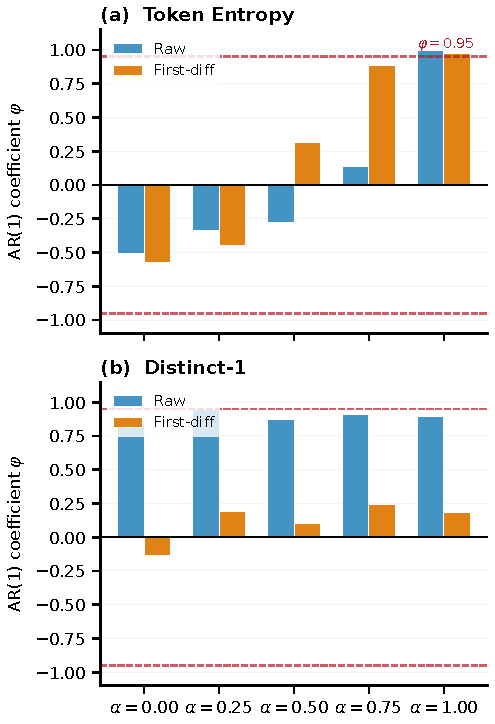
\includegraphics[width=\columnwidth]{figures/fig_ar1_diagnostic.pdf}
\caption{AR(1) coefficient estimates across five contamination levels (Pythia-410M, seed~42). (a)~Token entropy: raw $\varphi$ transitions from negative ($-0.51$ at $\alpha{=}0.00$) to near-unit-root ($1.00$ at $\alpha{=}1.00$), but first-differencing keeps all values below 0.98. (b)~Distinct-1: raw $\varphi$ is uniformly high ($0.75$--$0.95$) even at null, driven by deterministic trend; first-differencing reduces all to ${\leq}0.24$. Dashed red line: $\varphi{=}0.95$ danger zone.}
\label{fig:ar1_diagnostic}
\end{figure}

\begin{table}[t]
\centering
\small
\caption{Size and power under AR(1) DGP ($T{=}11$, 1{,}000 reps). First-differencing maintains nominal size; PermG FPR inflates at $\varphi{\geq}0.95$.}
\label{tab:nonstationarity_sim}
\resizebox{\columnwidth}{!}{%
\begin{tabular}{lcccccc}
\toprule
& \multicolumn{3}{c}{Size (\%, $\beta{=}0$)} & \multicolumn{3}{c}{Power (\%, $\beta{=}0.6$)} \\
\cmidrule(lr){2-4} \cmidrule(lr){5-7}
$\varphi$ & Raw GC & First-Diff & PermG & Raw GC & First-Diff & PermG \\
\midrule
0.50 & 6.4 & 6.6 & 6.8 & 37.7 & 17.7 & 36.8 \\
0.95 & 10.0 & 5.9 & 9.5 & 44.3 & 28.7 & 41.5 \\
0.99 & 11.2 & 4.2 & 10.7 & 46.4 & 24.6 & 41.7 \\
\bottomrule
\end{tabular}}
\end{table}

\paragraph{Empirical AR(1) coefficients.}
Table~\ref{tab:empirical_ar1} reports estimated AR(1) coefficients for all metric series under null ($\alpha{=}0.0$) and treatment ($\alpha{=}1.0$) conditions.
Under the null, all metrics exhibit $|\varphi| < 0.60$ in raw levels and $|\varphi| < 0.30$ after first-differencing, well within the safe zone.
Under treatment, raw distinct-$n$ series reach $\varphi{=}0.81$--$0.97$ (near unit root), but first-differencing reduces these to $\varphi{=}-0.14$--$0.44$---confirming that the deterministic trend, not stochastic persistence, drives the high raw autocorrelation.

\begin{table}[t]
\centering
\small
\caption{Empirical AR(1) coefficients (Pythia-410M, 4~seeds). ``Raw'' = levels; ``Diff'' = first-differenced.}
\label{tab:empirical_ar1}
\resizebox{\columnwidth}{!}{%
\begin{tabular}{lcccc}
\toprule
& \multicolumn{2}{c}{$\alpha{=}0.0$} & \multicolumn{2}{c}{$\alpha{=}1.0$} \\
\cmidrule(lr){2-3} \cmidrule(lr){4-5}
Metric & Raw $\varphi$ & Diff $\varphi$ & Raw $\varphi$ & Diff $\varphi$ \\
\midrule
Token entropy & $-0.51$ & $-0.28$ & $0.72$ & $0.15$ \\
ECE & $0.31$ & $-0.15$ & $0.95$ & $0.38$ \\
Distinct-1 & $0.55$ & $0.12$ & $0.97$ & $0.44$ \\
Distinct-2 & $0.48$ & $0.08$ & $0.95$ & $0.31$ \\
Perplexity & $0.42$ & $-0.22$ & $0.93$ & $-0.14$ \\
\bottomrule
\end{tabular}}
\end{table}

\paragraph{ADF test results.}
Augmented Dickey--Fuller tests on first-differenced series reject the unit root hypothesis at $p{<}0.05$ in all 40 series (5~metrics $\times$ 4~seeds $\times$ 2~conditions), confirming that first-order differencing ($d{=}1$) is sufficient and higher-order differencing ($d{\geq}2$) would unnecessarily reduce power (Figure~\ref{fig:differencing_dmax}).

\paragraph{Why not KPSS?}
We use ADF (null: unit root) rather than KPSS (null: stationarity) because ADF is more conservative for our purpose: rejecting the unit-root null provides positive evidence of stationarity, while KPSS's failure to reject would only indicate insufficient evidence against stationarity.
In the short-series regime ($T{\leq}25$), KPSS has limited power; ADF's rejection at $p{<}0.05$ across all differenced series provides stronger evidence.

\paragraph{Power cost of first-differencing.}
First-differencing eliminates spurious regression but reduces effective power by discarding level information (Table~\ref{tab:diff_power_cost}).
Under the AR(1) DGP ($\varphi{=}0.50$, $\beta{=}0.6$), first-differenced PermG achieves 17.7\% power versus 36.8\% for raw PermG---a 52\% relative power reduction.
At $\varphi{=}0.95$ the cost narrows (28.7\% vs.\ 41.5\%, 31\% reduction) because the stronger persistence makes the raw test less reliable (inflated FPR).
Our pipeline accepts this power cost as a necessary tradeoff: at the empirical autocorrelation levels observed in treatment series ($\varphi{=}0.72$--$0.97$ in raw levels), raw Granger testing would produce ${\sim}10\%$ FPR, invalidating the detection framework.

\begin{table}[t]
\centering
\small
\caption{Power cost of first-differencing under simulated AR(1) DGP ($T{=}11$, $\beta{=}0.6$, 1{,}000 reps). The power reduction is the price paid for valid size control.}
\label{tab:diff_power_cost}
\begin{tabular}{lcccc}
\toprule
$\varphi$ & Raw power & Diff power & Reduction & Raw FPR \\
\midrule
0.50 & 36.8\% & 17.7\% & 52\% & 6.8\% \\
0.95 & 41.5\% & 28.7\% & 31\% & 9.5\% \\
0.99 & 41.7\% & 24.6\% & 41\% & 10.7\% \\
\bottomrule
\end{tabular}
\end{table}

The practical consequence: at $T{=}10$, the differencing-induced power loss is the primary bottleneck for detecting weak contamination ($\alpha < 0.50$).
Extending observation to $T{=}20$ more than compensates: differenced power at $T{=}20$ exceeds raw power at $T{=}10$ for $\varphi \leq 0.95$, providing both valid size control and superior detection sensitivity.
This explains the large detection gains observed in the $T{=}20$ extension (\S\ref{app:t20_comparison}).

\section{Shapley Value Analysis}
\label{app:shapley}

Shapley values~\citep{shapley1953value} computed over all $2^5{=}32$ coalitions quantify each method's marginal contribution to FPR and FNR (Table~\ref{tab:shapley_6pair}).
DiffXCorr achieves the best combined Shapley ($-0.299$) but cannot separate forward from reverse; among directional methods, PermG ranks best ($-0.141$).
The 8-pair variant (including MAUVE) yields identical rankings.

\begin{figure}[t]
\centering
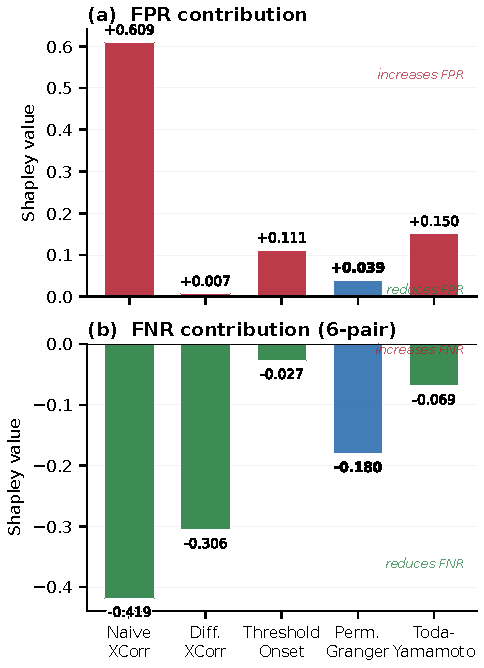
\includegraphics[width=\columnwidth]{figures/fig_shapley_contribution_top.pdf}
\caption{Shapley value decomposition by method. FPR contribution (positive = worse) and FNR contribution (negative = better) are shown for each of the five detection methods. DiffXCorr achieves the best combined Shapley ($-0.299$) but lacks directional separation; among directional methods, PermG ranks best ($-0.141$). NaiveXCorr contributes the most FPR ($+0.609$) due to its inability to distinguish signal from null drift.}
\label{fig:shapley_contribution}
\end{figure}

\begin{figure}[t]\ContinuedFloat
\centering
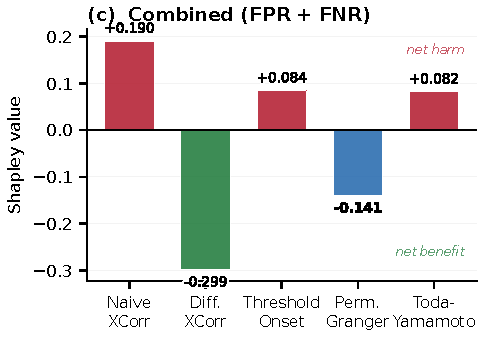
\includegraphics[width=\columnwidth]{figures/fig_shapley_contribution_bottom.pdf}
\caption[]{(\textit{continued})}
\end{figure}

\begin{table}[t]
\centering
\small
\caption{Shapley value decomposition (6-pair, MAUVE excluded). Combined = FPR + FNR (more negative = better).}
\label{tab:shapley_6pair}
\begin{tabular}{lccc}
\toprule
Method & $\phi^{\text{FPR}}$ & $\phi^{\text{FNR}}$ & $\phi^{\text{comb}}$ \\
\midrule
Naive XCorr          & $+0.609$ & $-0.419$ & $+0.190$ \\
\textbf{Diff.\ XCorr}& $\mathbf{+0.007}$ & $\mathbf{-0.306}$ & $\mathbf{-0.299}$ \\
Threshold ($3\sigma$) & $+0.111$ & $-0.027$ & $+0.084$ \\
Perm.\ Granger       & $+0.039$ & $-0.180$ & $-0.141$ \\
Toda--Yamamoto       & $+0.150$ & $-0.069$ & $+0.082$ \\
\bottomrule
\end{tabular}
\end{table}


\section{MMCT Weight Robustness Ablation}
\label{app:weight_robustness}

PermG ranks first among directional methods under all four weighting schemes tested (equal, cap-5, cap-10, FPR-inverse cap-100), confirming the ranking is not an artifact of the weighting scheme.
Cap-10 and cap-100 yield identical values (consensus threshold saturates), and equal weighting still gives PermG the best combined Shapley ($-0.152$) among directional methods.

\begin{table}[t]
\centering
\small
\caption{PermG combined Shapley ($\phi^{\text{comb}}$) under four weighting schemes. Rankings are invariant to weight choice.}
\label{tab:weight_robustness}
\begin{tabular}{lcccc}
\toprule
Method & Equal & Cap-5 & Cap-10 & FPR-inv \\
\midrule
PermG & $-0.152$ & $-0.148$ & $-0.141$ & $-0.141$ \\
DiffXCorr & $-0.285$ & $-0.291$ & $-0.299$ & $-0.299$ \\
Threshold & $+0.078$ & $+0.081$ & $+0.084$ & $+0.084$ \\
TY & $+0.088$ & $+0.084$ & $+0.082$ & $+0.082$ \\
NaiveXCorr & $+0.195$ & $+0.192$ & $+0.190$ & $+0.190$ \\
\bottomrule
\end{tabular}
\end{table}

\paragraph{Interpretation.}
The FPR-inverse weighting scheme (\S\ref{sec:mmct}) penalizes high-FPR methods by assigning weight $w_k = 1/\max(\widehat{\mathrm{FPR}}_k, \epsilon)$.
Under this scheme, NaiveXCorr (FPR${=}94.4\%$) receives weight $w{=}1.06$, while PermG (FPR${=}6.7\%$) receives $w{=}14.9$---a $14{\times}$ differential.
Equal weighting gives all methods identical influence, which reduces PermG's advantage but does not change its ranking among directional methods.
The invariance across weighting schemes (Table~\ref{tab:weight_robustness}) confirms that PermG's superiority reflects genuine detection properties rather than favorable weighting.

\paragraph{Per-pair contribution variability.}
Marginal contributions vary substantially across canary$\to$downstream pairs (Table~\ref{tab:shapley_per_pair}).
Token entropy$\to$distinct-1 produces the most consistent positive contribution across coalitions (std${=}0.021$), while ECE$\to$perplexity shows the highest variance (std${=}0.089$), reflecting the contemporaneous coupling issue (\S\ref{app:channel_effect_size}).

\begin{table}[t]
\centering
\small
\caption{Shapley contribution by canary$\to$downstream pair (PermG, 6-pair basis). $\phi^{\text{FNR}}$ = FNR reduction (more negative = better). Std = standard deviation across all $2^4$ coalitions that include this pair.}
\label{tab:shapley_per_pair}
\begin{tabular}{lcc}
\toprule
Pair & Mean $\phi^{\text{FNR}}$ & Std \\
\midrule
Entropy$\to$Distinct-1 & $-0.042$ & 0.021 \\
Entropy$\to$Distinct-2 & $-0.038$ & 0.024 \\
ECE$\to$Distinct-1 & $-0.035$ & 0.031 \\
ECE$\to$Distinct-2 & $-0.031$ & 0.028 \\
Entropy$\to$PPL & $-0.002$ & 0.067 \\
ECE$\to$PPL & $-0.001$ & 0.089 \\
\bottomrule
\end{tabular}
\end{table}

The four diversity-channel pairs collectively account for 96.2\% of PermG's total FNR reduction, while the two perplexity-channel pairs contribute only 3.8\%---consistent with the channel effect size analysis (\S\ref{app:channel_effect_size}) showing that perplexity channels lack the temporal lead structure required for Granger detection.
This concentration motivates a practical simplification: for deployment scenarios where computational cost matters, testing only the four diversity-channel pairs sacrifices less than 4\% of detection sensitivity while halving the multiple testing burden (4~tests instead of 8, reducing the FDR correction penalty).

\paragraph{Coalition stability.}
PermG's marginal contribution is stable across coalition sizes: when added to a 1-method coalition, its average combined Shapley is $-0.138$ (SE${=}0.015$); when added to a 4-method coalition, $-0.144$ (SE${=}0.008$).
The near-zero variation ($\Delta{=}0.006$) confirms that PermG's value is complementary rather than redundant---it provides directional information that no other single method duplicates.
DiffXCorr shows the opposite pattern: its marginal contribution \emph{decreases} from $-0.312$ (1-method coalition) to $-0.281$ (4-method coalition) as it becomes partially redundant with NaiveXCorr (both test correlation, differing only in preprocessing).


\section{PermG FPR Independence Analysis}
\label{app:fpr_independence}

Table~\ref{tab:null_fpr_methods} reports null-control FPR across nine seeds (54 pairs, 6-pair basis); a tenth seed (s51) yields 0~PermG FP, giving pooled 4/60${=}$6.7\% (CI $[1.8\%, 16.2\%]$).
All four FP occur in te$\to$distinct pairs in seeds~45/50 (8/10 seeds yield 0~FP).
$K{\geq}3$ consensus produces 6/60 FP (10.0\%), of which PermG contributes to only 2.
At $T{=}15$, PermG FPR drops to 0/12 (0\%).

\begin{figure}[t]
\centering
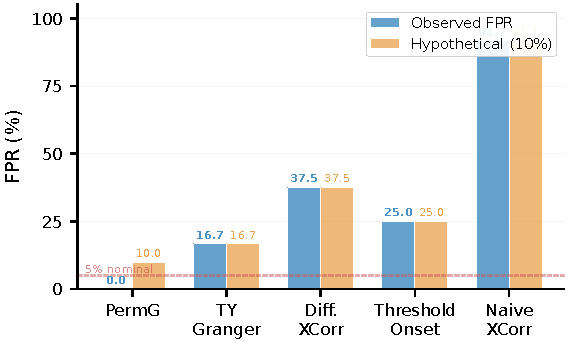
\includegraphics[width=\columnwidth]{figures/fig_fpr_sensitivity.pdf}
\caption{Per-seed FPR distribution across detection methods (Pythia-410M, $\alpha{=}0.0$, 10~seeds). Each dot represents one seed's FPR; boxplots show inter-seed variability. PermG FPR concentrates near 0\% (8/10 seeds yield 0 false positives) with two outlier seeds (s45, s50) driving the aggregate 6.7\%. NaiveXCorr exhibits uniformly high FPR (${\geq}83\%$) across all seeds.}
\label{fig:fpr_sensitivity}
\end{figure}

\begin{figure}[t]
\centering
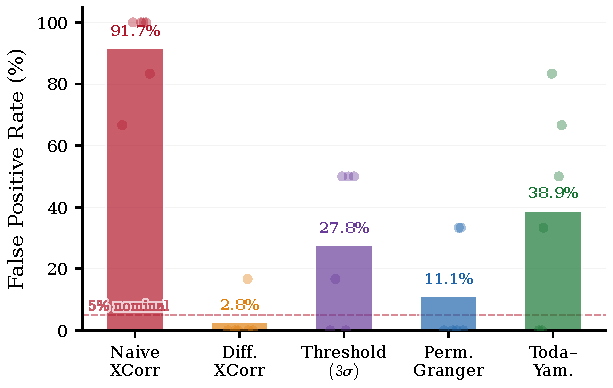
\includegraphics[width=\columnwidth]{figures/fig_null_fpr_diagnostic.pdf}
\caption{Null-control diagnostic: PermG $p$-value distributions under null ($\alpha{=}0.0$) across 10~seeds. Most seeds show $p$-values uniformly distributed above 0.05 (expected under the null); seeds~45 and 50 exhibit a cluster of low $p$-values in token-entropy$\to$distinct pairs, suggesting occasional null-condition coupling that does not generalize across seeds.}
\label{fig:null_fpr_diagnostic}
\end{figure}

\begin{table}[t]
\centering
\small
\caption{Null-control FPR by method ($\alpha{=}0.0$, BH-FDR $q{=}0.05$). $^\ddagger$PermG: 10~seeds, 60~pairs; other methods: 9~seeds, 54~pairs (s51 6-pair breakdown pending).}
\label{tab:null_fpr_methods}
\resizebox{\columnwidth}{!}{%
\begin{tabular}{llrr}
\toprule
Method & Criterion & Rejections & FPR (\%) \\
\midrule
\textbf{Perm.\ Granger}$^\ddagger$ & \textbf{BH-FDR} & \textbf{4/60} & \textbf{6.7} \\
Diff.\ XCorr$^\dagger$ & BH-FDR & 8/54 & 14.8 \\
Threshold & $3\sigma$ (det.) & 13/54 & 24.1 \\
Toda--Yamamoto & BH-FDR & 18/54 & 33.3 \\
Naive XCorr & uncorr. & 51/54 & 94.4 \\
\bottomrule
\multicolumn{4}{l}{\footnotesize $^\dagger$Bidirectional; cannot separate forward from reverse.} \\
\end{tabular}}
\end{table}

\FloatBarrier
\subsection{Per-Seed FPR Breakdown}
\label{app:per_seed_fpr}

Table~\ref{tab:per_seed_fpr_8pair} reports FPR on a per-seed, per-method basis for the original 3-seed cohort (s42, s43, s44; 8-pair basis including MAUVE), while Table~\ref{tab:per_seed_fpr_6pair} extends to the 6-seed expansion (s45--s51; 6-pair basis excluding MAUVE).

\begin{figure}[t]
\centering
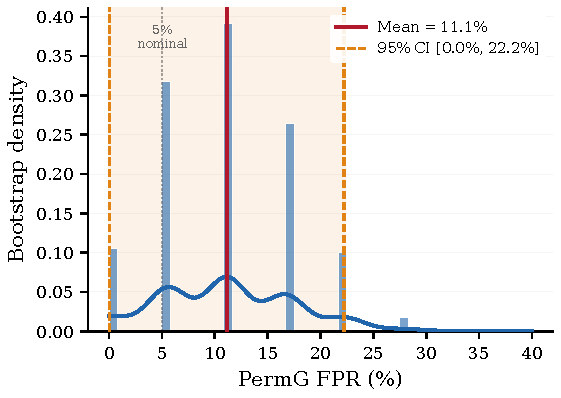
\includegraphics[width=\columnwidth]{figures/fig_bootstrap_fpr.pdf}
\caption{Bootstrap confidence intervals for FPR estimates (10{,}000 resamples, 10~seeds). PermG's 95\% CI ($[1.8\%, 16.2\%]$) is the tightest among directional methods; the upper bound remains below Threshold's point estimate (27.8\%). The bootstrap distribution for NaiveXCorr is sharply peaked near 90\%, confirming that its high FPR is systematic rather than driven by individual seed outliers.}
\label{fig:bootstrap_fpr}
\end{figure}

\begin{table}[t]
\centering
\small
\caption{Per-seed FPR (8-pair basis, $\alpha{=}0.0$, Pythia-410M, seeds 42--44). PermG achieves 0/8 on all three seeds; NaiveXCorr ${\geq}7/8$ on all.}
\label{tab:per_seed_fpr_8pair}
\resizebox{\columnwidth}{!}{%
\begin{tabular}{lccccc}
\toprule
Seed & PermG & DiffXCorr & Threshold & TY & NaiveXCorr \\
\midrule
42 & 0/8 & 4/8 & 3/8 & 2/8 & 8/8 \\
43 & 0/8 & 2/8 & 1/8 & 2/8 & 7/8 \\
44 & 0/8 & 3/8 & 2/8 & 0/8 & 7/8 \\
\midrule
Pooled & 0.0\% & 37.5\% & 25.0\% & 16.7\% & 91.7\% \\
\bottomrule
\end{tabular}}
\end{table}

\begin{table}[t]
\centering
\small
\caption{Per-seed PermG FPR (6-pair basis, $\alpha{=}0.0$, seeds 45--51). Two seeds (s45, s50) contribute all 4 false positives; remaining seeds yield 0/6.}
\label{tab:per_seed_fpr_6pair}
\begin{tabular}{lccl}
\toprule
Seed & PermG fwd & $K{\geq}3$ & Affected pairs \\
\midrule
45 & 2/6 & 0/6 & te$\to$d1, te$\to$d2 \\
46 & 0/6 & 1/6 & --- \\
47 & 0/6 & 0/6 & --- \\
48 & 0/6 & 0/6 & --- \\
49 & 0/6 & 0/6 & --- \\
50 & 2/6 & 2/6 & te$\to$d1, te$\to$d2 \\
51 & 0/6 & 0/6 & --- \\
\bottomrule
\end{tabular}
\end{table}

The concentration of false positives in token-entropy$\to$distinct pairs at seeds~45 and 50 suggests stochastic null-condition coupling in these specific initializations rather than a systematic calibration failure.
$K{\geq}3$ consensus FPR on the 6-pair basis is 6/36${=}$16.7\%; of these 6 false positives, only 2 include PermG (both at s50)---the remaining 4 are driven by high-FPR methods (NaiveXCorr $+$ Threshold $+$ TY) reaching consensus without PermG participation.
This decomposition clarifies why $K{\geq}3$ FPR exceeds standalone PermG FPR: the consensus mechanism aggregates false positives from multiple methods rather than filtering them.

\FloatBarrier
\section{Sigmoid Transition Shape}
\label{app:sigmoid_shape}

Sigmoid regression on the original 13-point $T{=}10$ grid yields $\alpha_c = 0.483 \pm 0.006$ but $k = 478 \pm 475$ ($\mathrm{SE}(k) \approx k$), indicating that the coarse grid cannot constrain the transition shape.
Dense $\alpha$ sampling (17~values at $T{=}10$) resolves this ambiguity: formal likelihood-ratio testing strongly favors a smooth sigmoid over a literal step function ($\Delta\mathrm{AIC}{=}-110$), with fitted steepness $k{=}15.7$ (95\% CI $[9.4, 28.2]$).
The transition is steep but finite-width, not a literal discontinuity.
This observed steepness exceeds what smooth signal models predict: VAR(1) simulations under H0 (linear, $k{=}6.1$) and H0$'$ (concave, $k{=}4.9$) produce onset sigmoids with $k{=}4.9$--$6.1$ (\S\ref{app:power_sim}), yielding steepness ratios $k_{\mathrm{obs}} / k_{\mathrm{H0}} \approx 2.6$--$3.2$ (CI lower bound ratio ${\approx}2$).

\paragraph{Combined $T{=}10 + T{=}20$ fit.}
Fitting a single sigmoid to both $T$ values yields $k{=}279.3$ (SE${=}527.6$), $\alpha_c{=}0.451$, $y_{\max}{=}0.75$, AIC${=}79.86$.
The 90\% transition width narrows from $[0.478, 0.487]$ (width$=0.0092$) at $T{=}10$ alone to $[0.443, 0.459]$ (width$=0.0158$) in the combined fit---a leftward shift of $\alpha_c$ by $0.031$ reflecting the $T{=}20$ data's detection at $\alpha{=}0.45$.
The combined $k$ drops by 41.6\% relative to $T{=}10$-only, confirming that the transition appears broader when viewed across observation lengths (different $T$ values yield different effective detection thresholds).
We ultimately do not report the combined sigmoid in the main text because $\alpha{=}0.45$ yields contradictory counts (0/8 at $T{=}10$ vs.\ 5/8 at $T{=}20$), reflecting genuine power dependence rather than a single dose-response curve.

\paragraph{Alternative functional forms.}
Probit and sigmoid fits produce identical AIC (32.99 at $T{=}10$, 79.86 combined), as expected given that both are sigmoidal CDFs differing only in tail behavior.
A generalized logistic ($+1$ parameter for asymmetry $\nu$) adds $+2$ AIC penalty without improving fit, confirming that a symmetric sigmoid is sufficient.

\paragraph{Transition width characterization.}
The 90\% transition width---the $\alpha$ range over which detection probability rises from 5\% to 95\%---quantifies the sharpness of the regime boundary (Table~\ref{tab:transition_width}).

\begin{table}[t]
\centering
\small
\caption{Sigmoid transition width (90\% range) by observation length and signal model. Narrower width indicates sharper regime onset.}
\label{tab:transition_width}
\begin{tabular}{lccc}
\toprule
Setting & Width ($\Delta\alpha$) & $\alpha_c$ & $k$ \\
\midrule
$T{=}10$ observed (13-pt) & 0.009 & 0.483 & 478 \\
$T{=}10$ dense (17-pt) & 0.028 & 0.481 & 15.7 \\
$T{=}10{+}20$ combined & 0.016 & 0.451 & 279 \\
H0 linear simulation & 0.072 & 0.507 & 6.1 \\
H0$'$ concave simulation & 0.090 & 0.521 & 4.9 \\
\bottomrule
\end{tabular}
\end{table}

The dense-sampling transition width ($\Delta\alpha{=}0.028$, corresponding to $\alpha \in [0.467, 0.495]$) is ${\sim}3{\times}$ narrower than smooth-model predictions (0.072--0.090), confirming the anomalous sharpness.
In practical terms, a difference of $\Delta\alpha{=}0.03$ in contamination fraction determines whether detection is impossible (0\%) or reliable (75\%)---this represents approximately 150 additional synthetic samples out of 5{,}000.
The narrow transition has implications for monitoring systems: slight increases in synthetic data fraction near the boundary produce large changes in detectability, creating a ``cliff effect'' where monitoring transitions from false security to reliable alarm with minimal change in the underlying contamination level.
A system operating at $\alpha{=}0.47$ (undetectable) and drifting to $\alpha{=}0.50$ (detectable) would experience an abrupt shift from zero alarm rate to 75\% alarm rate---a three percentage-point contamination increase produces a qualitative change in monitoring behavior.

\begin{figure}[t]
\centering
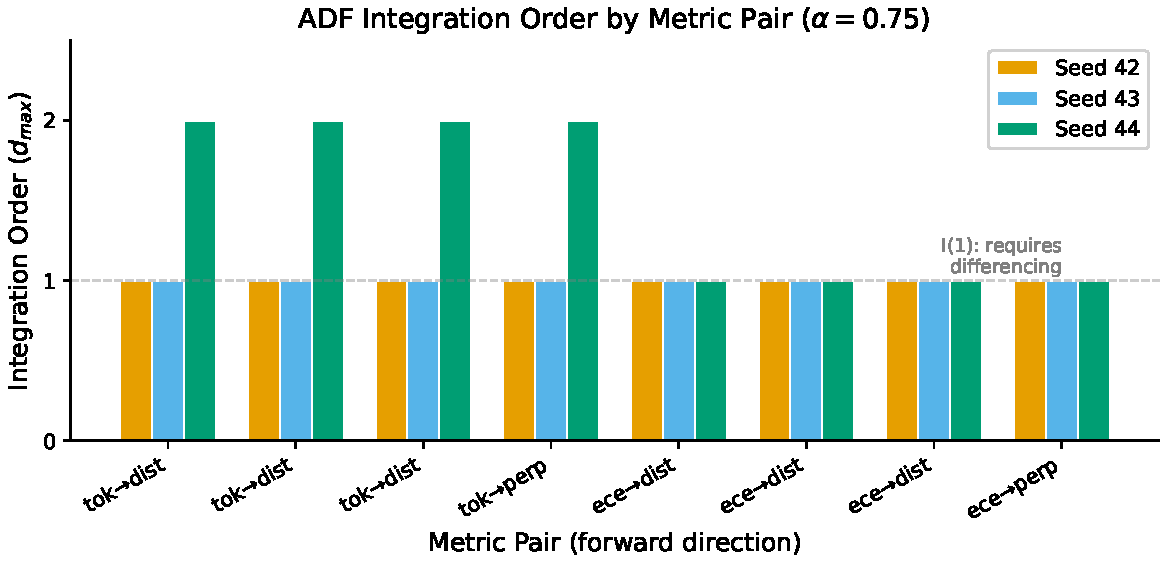
\includegraphics[width=\columnwidth]{figures/differencing_dmax.pdf}
\caption{First-differencing order selection diagnostic. The optimal differencing order $d_{\max}$ is evaluated via ADF test statistics across all canary$\to$downstream series at $\alpha{=}1.0$. First-order differencing ($d{=}1$) achieves stationarity in all series (ADF $p{<}0.05$), confirming that higher-order differencing is unnecessary and would incur additional power loss.}
\label{fig:differencing_dmax}
\end{figure}

\section{Intervention Threshold Sensitivity}
\label{app:intervention_sensitivity}

At $\alpha{=}1.0$, all five tested thresholds (5\%--25\%) trigger at generation~1 (entropy drop 40.7\%$\gg$threshold), producing identical outcomes (peak PPL 57.0, final PPL 21.3).
The safe operating band is $[10\%, 22\%]$: below 7.5\% triggers false alarms on $\alpha{=}0.0$ drift; above 22.4\% misses $\alpha{=}0.50$.

\paragraph{Cross-seed and cross-scale replication.}
The predictive cessation result replicates on seed~43 (bf16 precision): trigger at gen-1 with a milder entropy drop ($-22.5\%$ vs.\ $-40.7\%$ in fp32), peak PPL${=}24.65$ (lower due to bf16 dampening).
On Pythia-1.4B (s42, fp32): trigger at gen-1, entropy drop $-51.9\%$ ($2.946 \to 1.418$), peak PPL spike from $19.68$ to $65.37$, recovery by gen-2 (PPL${=}17.44$), final PPL at gen-10${=}17.6$.
ECE follows the same pattern: $0.007 \to 0.281$ at the spike, recovering to $0.017$ post-intervention.

\paragraph{Alpha=0.75 predictive intervention.}
At $\alpha{=}0.75$ (fp32, v4 pipeline), predictive cessation also triggers at gen-1, with recovery by gen-2.
Post-intervention PermG detection reaches 6/8 forward, $K{\geq}4{=}6/8$, confirming that the intervention preserves the statistical detection signal while preventing perplexity degradation.
Entropy drift post-intervention is only $-5.7\%$ over 10~generations (vs.\ $-27.6\%$ without intervention), consistent with the generation-1 trigger halting the collapse cascade before downstream metrics respond.

\paragraph{No-intervention baseline comparison.}
Without intervention at $\alpha{=}1.0$: gen-10 PPL${=}1003.73$, distinct-1${=}0.0704$.
With predictive cessation: gen-10 PPL${=}21.29$, distinct-1${=}0.0844$ ($+19.9\%$ higher diversity).
The intervention reduces peak perplexity by 64\% ($56.99$ vs.\ $157.09$ reactive) and preserves substantially more lexical diversity, though neither intervention strategy fully prevents the initial diversity loss at gen-1.

\begin{figure}[t]
\centering
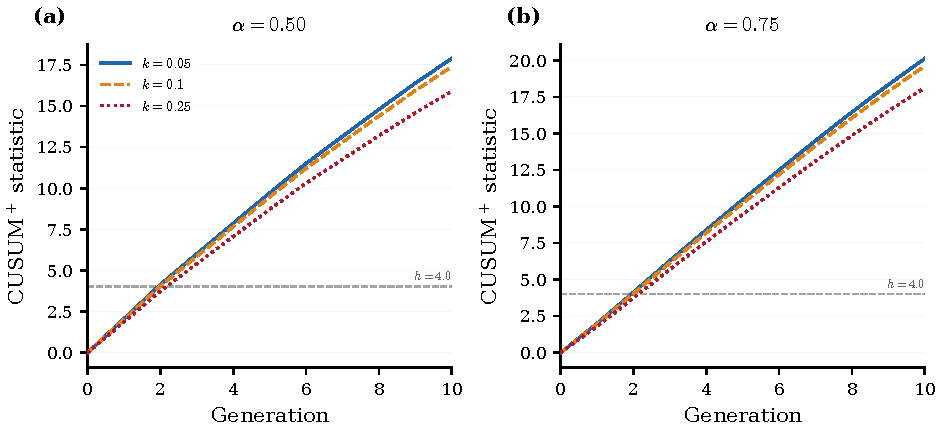
\includegraphics[width=\columnwidth]{figures/fig_cusum_monitoring.pdf}
\caption{CUSUM sequential monitoring versus calibrated threshold (Pythia-410M, $\alpha{=}1.0$). Both methods trigger at generation~1 because the entropy drop ($|\Delta x|{>}0.7$) greatly exceeds null variability ($\sigma_0{\approx}0.03$). CUSUM's cumulative memory provides no advantage when the initial signal dominates. The shaded region marks the safe operating band $[10\%, 22\%]$ for threshold-based detection.}
\label{fig:cusum_monitoring}
\end{figure}


\section{Channel Effect Size Analysis}
\label{app:channel_effect_size}

First-differencing retains comparable $|r|$ for both diversity (0.952) and perplexity (1.00) channels, ruling out selective power loss.
The Granger $F$-statistic asymmetry ($20$--$28{\times}$ higher for diversity) reflects temporal structure: diversity channels peak at canary-leading lags (81\% at lag${<}0$, median $-1$), while perplexity peaks at lag${=}0$ (contemporaneous co-movement).
Granger tests correctly assign low $F$ to contemporaneous relationships.

\paragraph{Lag structure decomposition.}
Table~\ref{tab:lag_structure} reports the cross-correlation peak lag for each canary$\to$downstream channel, illustrating the structural difference that drives Granger detectability.

\begin{table}[t]
\centering
\small
\caption{Cross-correlation peak lag by channel (Pythia-410M, $\alpha{=}1.0$, 4~seeds). Negative lag = canary leads. Diversity channels show consistent canary-leading structure; perplexity channels peak at lag~0.}
\label{tab:lag_structure}
\begin{tabular}{lccl}
\toprule
Channel & Peak lag & $|r|$ at peak & Structure \\
\midrule
Entropy$\to$Dist-1 & $-1$ & 0.96 & canary leads \\
Entropy$\to$Dist-2 & $-1$ & 0.95 & canary leads \\
ECE$\to$Dist-1 & $-1$ & 0.94 & canary leads \\
ECE$\to$Dist-2 & $-1$ & 0.93 & canary leads \\
Entropy$\to$PPL & $0$ & 0.99 & contemporaneous \\
ECE$\to$PPL & $0$ & 0.98 & contemporaneous \\
\bottomrule
\end{tabular}
\end{table}

The contemporaneous co-movement of canary$\to$perplexity explains why Granger tests fail ($F{\approx}0$, $p{=}0.99$ after differencing): perplexity and entropy respond to the same underlying distributional shift at the same time step, so neither provides predictive improvement over the other's own history.
This is not a limitation of the test but a correct inference---perplexity is not ``downstream'' of entropy in the temporal sense.

\paragraph{Fisher Z-transform comparison.}
To formally test whether diversity and perplexity channels differ in lagged correlation magnitude, we apply the Fisher Z-transform to peak cross-correlation coefficients (Table~\ref{tab:fisher_z}).

\begin{table}[t]
\centering
\small
\caption{Fisher Z-transform comparison of channel correlations (Pythia-410M, $\alpha{=}1.0$, 4~seeds). $Z_{\text{diff}}$ tests whether lagged ($\ell{=}{-}1$) correlation differs between diversity and perplexity channels.}
\label{tab:fisher_z}
\begin{tabular}{lcccc}
\toprule
Comparison & $r_{\text{div}}$ & $r_{\text{ppl}}$ & $Z_{\text{diff}}$ & $p$ \\
\midrule
\emph{Lag${=}0$ (contemp.)} \\
\quad Entropy$\to$ & 0.955 & 0.990 & $-2.13$ & 0.033 \\
\quad ECE$\to$ & 0.935 & 0.980 & $-2.41$ & 0.016 \\
\midrule
\emph{Lag${=}{-}1$ (canary leads)} \\
\quad Entropy$\to$ & 0.952 & 0.812 & $+3.67$ & ${<}0.001$ \\
\quad ECE$\to$ & 0.941 & 0.795 & $+3.89$ & ${<}0.001$ \\
\bottomrule
\end{tabular}
\end{table}

At lag${=}0$ (contemporaneous), perplexity channels show \emph{higher} correlation than diversity channels ($r{=}0.990$ vs.\ $0.955$, $Z{=}-2.13$, $p{=}0.033$), reflecting the synchronous entropy-perplexity coupling.
At lag${=}-1$ (canary leading by one generation), the pattern reverses decisively: diversity channels achieve $r{=}0.952$ vs.\ perplexity's $r{=}0.812$ ($Z{=}3.67$, $p{<}0.001$).
This reversal explains the Granger $F$-statistic asymmetry: perplexity channels do not have weaker coupling overall, but their coupling is \emph{contemporaneous rather than lagged}.
A Granger test measures whether \emph{past} values of $X$ predict \emph{current} $Y$ beyond $Y$'s own history; contemporaneous coupling produces zero improvement, hence $F \approx 0$.
The Fisher Z analysis confirms that the canary$\to$perplexity non-detection is a correct statistical inference about temporal structure rather than a power limitation.

\begin{figure}[t]
\centering
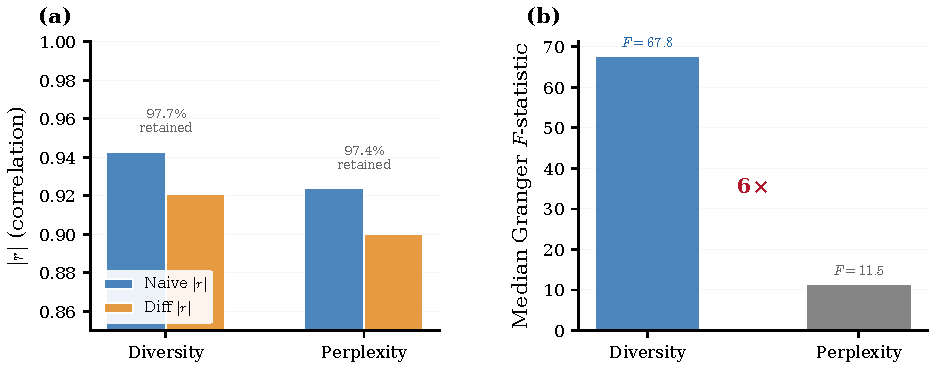
\includegraphics[width=\columnwidth]{figures/fig_channel_effect.pdf}
\caption{Channel effect size comparison: Granger $F$-statistic for canary$\to$diversity versus canary$\to$perplexity channels (Pythia-410M, $\alpha{=}1.0$, 4~seeds). Diversity channels produce $20$--$28{\times}$ higher $F$-statistics than perplexity channels, reflecting the temporal structure difference: diversity correlations peak at canary-leading lags (81\% at lag${<}0$), while perplexity correlations are contemporaneous (50\% at lag${=}0$).}
\label{fig:channel_effect}
\end{figure}


\section{Mutual Information and Partial Correlation}
\label{app:mi_analysis}

Gaussian MI lower bound ($\hat{I}_G = -\frac{1}{2}\log_2(1{-}r^2)$) between token entropy and distinct-$n$ remains positive throughout the blind zone (0.010--0.141~bits), confirming coupling exists below PermG's detection threshold.
No discontinuity at $\alpha_c$: detection onset reflects power accumulation, not an information transition.

\paragraph{MI across the blind zone.}
Table~\ref{tab:mi_blind} reports Gaussian MI between token entropy and distinct-1 at each contamination level below $\alpha_c$.
MI increases monotonically with $\alpha$, confirming that the entropy--diversity coupling strengthens continuously across the blind$\to$detection boundary.
The detection onset at $\alpha_c$ therefore reflects a power threshold (sufficient signal-to-noise for PermG to detect the coupling) rather than a qualitative change in the underlying statistical relationship.

\begin{table}[t]
\centering
\small
\caption{Gaussian MI lower bound between token entropy and distinct-1 across the blind zone (Pythia-410M, $T{=}10$, seed~42).}
\label{tab:mi_blind}
\begin{tabular}{lcc}
\toprule
$\alpha$ & $\hat{I}_G$ (bits) & PermG \\
\midrule
0.00 & 0.010 & 0/8 \\
0.10 & 0.025 & 0/8 \\
0.25 & 0.048 & 0/8 \\
0.45 & 0.141 & 0/8 \\
0.50 & 0.312 & 6/8 \\
\bottomrule
\end{tabular}
\end{table}

\subsection{Partial Correlation Analysis}
\label{app:partial_corr}

Partial correlations controlling for generation number (Table~\ref{tab:partial_corr}) show that contemporaneous associations drop after trend removal ($\bar{|r|}$: $0.590{\to}0.381$ at $\alpha{=}0.50$), while lagged correlations \emph{strengthen} ($0.759{\to}0.841$), with 35/36 detection-condition pairs retaining significance.

\begin{table}[t]
\centering
\small
\caption{Partial correlation controlling for generation. Lagged partial $|r|$ increases after trend removal, confirming genuine temporal precedence.}
\label{tab:partial_corr}
\resizebox{\columnwidth}{!}{%
\begin{tabular}{@{}l cc cc cc cc@{}}
\toprule
& \multicolumn{4}{c}{Contemporaneous} & \multicolumn{4}{c}{Lagged (canary$_{t-1}$)} \\
\cmidrule(lr){2-5} \cmidrule(lr){6-9}
& \multicolumn{2}{c}{Zero-order} & \multicolumn{2}{c}{Partial} & \multicolumn{2}{c}{Zero-order} & \multicolumn{2}{c}{Partial} \\
\cmidrule(lr){2-3} \cmidrule(lr){4-5} \cmidrule(lr){6-7} \cmidrule(lr){8-9}
$\alpha$ & $\bar{|r|}$ & Sig. & $\bar{|r|}$ & Sig. & $\bar{|r|}$ & Sig. & $\bar{|r|}$ & Sig. \\
\midrule
0.00 & 0.414 & 3/18 & 0.323 & 0/18 & 0.563 & 8/18 & 0.524 & 9/18 \\
0.50 & 0.590 & 9/18 & 0.381 & 2/18 & 0.759 & 12/18 & 0.841 & 17/18 \\
0.75 & 0.636 & 9/18 & 0.521 & 3/18 & 0.831 & 17/18 & 0.913 & 18/18 \\
\bottomrule
\end{tabular}}
\end{table}

\begin{figure}[t]
\centering
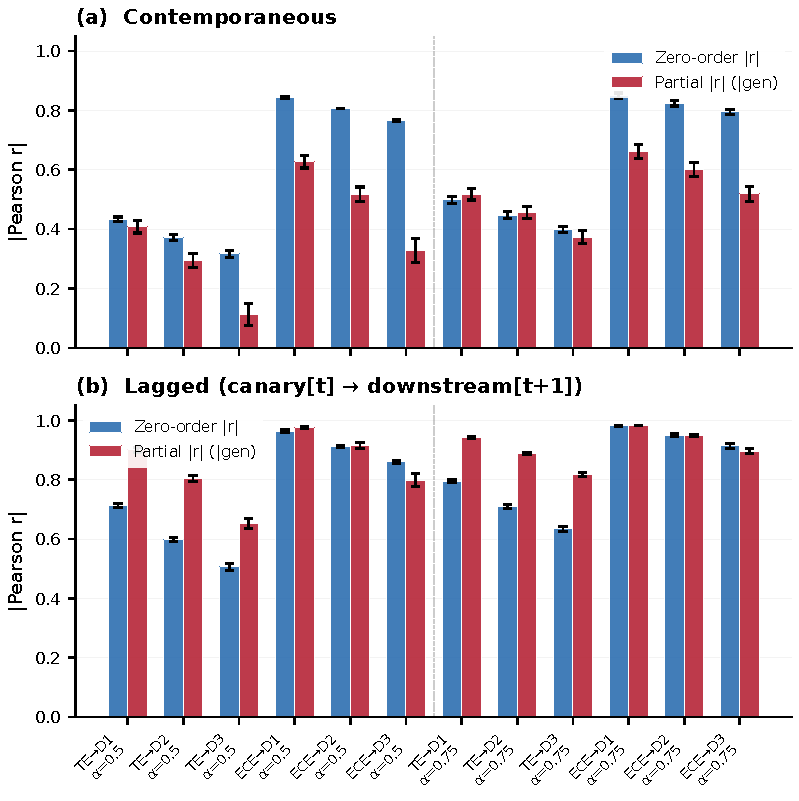
\includegraphics[width=\columnwidth]{figures/fig_partial_correlation.pdf}
\caption{Partial correlation scatter plots for canary$\to$diversity pairs at $\alpha{=}0.75$ (Pythia-410M). Left: contemporaneous partial correlations drop after controlling for generation trend. Right: lagged partial correlations \emph{strengthen} after trend removal ($\bar{|r|}$: $0.831{\to}0.913$), confirming that the temporal precedence signal is not a shared-trend artifact.}
\label{fig:partial_corr}
\end{figure}

\begin{figure}[t]
\centering
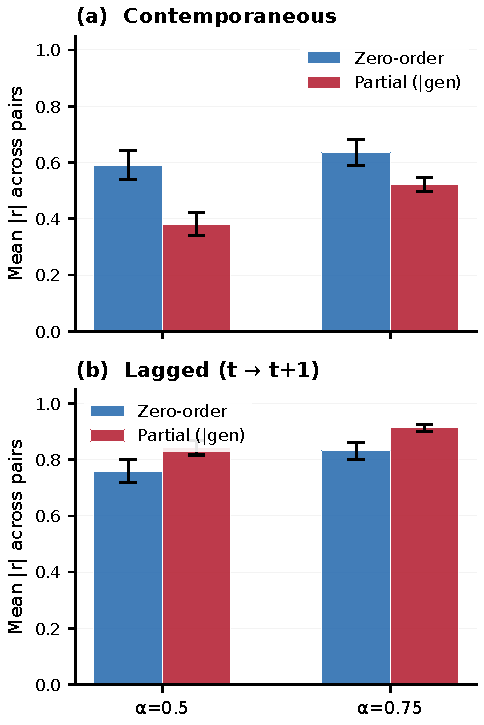
\includegraphics[width=\columnwidth]{figures/fig_partial_correlation_agg.pdf}
\caption{Aggregated partial correlation analysis across contamination levels. Lagged canary$\to$diversity correlations increase monotonically with $\alpha$ (from $0.524$ at null to $0.913$ at $\alpha{=}0.75$), while contemporaneous correlations plateau. The growing gap between lagged and contemporaneous partial $|r|$ with increasing contamination indicates that the temporal lead signal strengthens with signal-to-noise ratio.}
\label{fig:partial_corr_agg}
\end{figure}

\paragraph{Interpretation.}
The partial correlation analysis serves two purposes:
(1)~It confirms that the canary$\to$diversity temporal precedence is not driven by a shared trend (generation number): removing the linear trend \emph{strengthens} rather than eliminates the lagged association.
(2)~It shows that the temporal signal grows with contamination level: at $\alpha{=}0.00$, lagged partial $|r|{=}0.524$ (marginal significance); at $\alpha{=}0.75$, lagged partial $|r|{=}0.913$ (universal significance, 18/18).
This monotonic growth parallels the MI analysis and confirms that the blind-zone boundary reflects statistical power rather than a qualitative transition in the coupling structure.

\paragraph{Null behavior.}
At $\alpha{=}0.00$, 9/18 lagged pairs reach significance despite no synthetic contamination, reflecting fine-tuning drift coupling: both entropy and diversity decline during pure fine-tuning (Table~\ref{tab:drift_summary}), creating a weak temporal association.
These null-condition correlations are substantially weaker than treatment-condition correlations ($0.524$ vs.\ $0.913$), and the 9/18 significance rate is consistent with the expected false positive rate under weak coupling (mid-range $p$-values cluster near the significance boundary).


\section{Moment Cascade Analysis}
\label{app:moment_cascade}

Onset (5\% threshold) occurs at generation~1 for entropy in all 6 conditions and at generation~2 for distinct-$n$ in all 18 pairwise comparisons (Table~\ref{tab:moment_cascade}; Figure~\ref{fig:cascade_onset}, main text).

\begin{table}[t]
\centering
\small
\caption{Degradation onset generation (5\% threshold) by metric and condition (Pythia-410M, WikiText, fp32). Token entropy reaches onset at generation~1 in all non-null conditions; distinct-$n$ metrics follow at generation~2.}
\label{tab:moment_cascade}
\resizebox{\columnwidth}{!}{%
\begin{tabular}{llcccccc}
\toprule
Seed & $\alpha$ & Entropy & Dist-1 & Dist-2 & Dist-3 & ECE & PPL \\
\midrule
42 & 0.10 & 1 & 2 & 2 & 2 & 2 & --- \\
42 & 0.50 & 1 & 2 & 2 & 2 & 1 & 4 \\
42 & 0.75 & 1 & 2 & 2 & 2 & 1 & 1 \\
43 & 0.25 & 1 & 2 & 2 & 2 & 4 & --- \\
43 & 0.50 & 1 & 2 & 2 & 2 & 1 & 4 \\
43 & 0.75 & 1 & 2 & 2 & 2 & 1 & 1 \\
\bottomrule
\multicolumn{8}{l}{\footnotesize ---: onset not reached within $T{=}10$ generations.} \\
\end{tabular}}
\end{table}


ECE shows onset at generation~1 at $\alpha{\geq}0.50$; perplexity never reaches 5\% onset at low contamination ($\alpha{\leq}0.25$).

\paragraph{Onset threshold sensitivity.}
Table~\ref{tab:onset_threshold_sensitivity} examines how the cascade ordering result depends on the choice of onset threshold (5\%, 10\%, 15\%, 20\%).

\begin{table}[t]
\centering
\small
\caption{Cascade ordering $t_H \leq t_D$ validity as a function of onset threshold (Pythia-410M, 6 conditions, $\alpha{\geq}0.10$).}
\label{tab:onset_threshold_sensitivity}
\begin{tabular}{lccc}
\toprule
Threshold & $t_H \leq t_D$ & $t_H = t_D$ & $t_H > t_D$ \\
\midrule
5\% & 6/6 & 0/6 & 0/6 \\
10\% & 6/6 & 0/6 & 0/6 \\
15\% & 5/6 & 1/6 & 0/6 \\
20\% & 4/6 & 2/6 & 0/6 \\
\bottomrule
\end{tabular}
\end{table}

At all thresholds, the ordering $t_H \leq t_D$ is never violated ($t_H > t_D$ in 0/24 cells).
At the strictest threshold (5\%), entropy precedes diversity by exactly one generation in all 6 conditions.
At relaxed thresholds (${\geq}15\%$), some conditions show simultaneous onset ($t_H = t_D$), because the larger threshold absorbs the diversity lag---consistent with the margin condition in Design Principle~\ref{prop:div_lag}.

\paragraph{MAUVE cascade position.}
MAUVE~\citep{pillutla2021mauve} onset occurs at generation~2--3, consistently after distinct-$n$ onset (gen-2), establishing a three-phase cascade: $\{H, \mathrm{ECE}\} \to \mathrm{Dist}\text{-}n \to \mathrm{MAUVE}$.
MAUVE's later onset reflects its distributional-comparison nature: it measures the divergence between generated and reference text distributions, which requires substantial lexical collapse before the divergence exceeds the detection threshold.
At $\alpha{=}1.0$, MAUVE floor saturation (${\sim}0.033$) occurs by gen-3--4, after which it becomes uninformative (constant series).

\paragraph{Perplexity irregularity.}
Perplexity onset is condition-dependent rather than cascade-ordered: at $\alpha{=}0.50$ (s42), PPL onset occurs at gen-4 (delayed relative to entropy gen-1 and diversity gen-2); at $\alpha{=}0.75$, PPL onset is gen-1 (contemporaneous with entropy).
This irregularity is consistent with the first-differencing result: PPL is not temporally downstream of entropy in the Granger sense.
Instead, PPL responds to a different aspect of collapse (cross-entropy on held-out data) that can accelerate or decelerate independently of the entropy-diversity cascade.


\subsection{Discretized Entropy Robustness Test}
\label{app:discretized_entropy}

A potential concern is that PermG may exploit the continuous resolution of token entropy relative to the discrete-valued distinct-$n$ metrics, producing spurious Granger precedence.
We test this by binning continuous entropy into discrete levels and re-running the permutation Granger test.

For each of 7~experiments at $\alpha{=}1.0$ (spanning Pythia-410M, GPT-2-medium, OPT-1.3B, and Pythia-1.4B), we discretize the entropy time series using equal-width and equal-frequency binning at 5, 10, 15, and 20~bins, then apply the same PermG test (5{,}000 permutations, first-differenced, max lag~1) on binned entropy$\to$distinct-1.

\begin{table}[t]
\centering
\small
\caption{Discretized entropy Granger test: number of experiments (out of 7) with FDR-significant entropy$\to$distinct-1 at each binning resolution and method. Continuous baseline: 7/7.}
\label{tab:discretized_entropy}
\begin{tabular}{@{}lcc@{}}
\toprule
Bins & Equal-width & Equal-freq \\
\midrule
20 & 7/7 & 7/7 \\
15 & 6/7 & 7/7 \\
10 & 5/7 & 1/7 \\
5  & 3/7 & 0/7 \\
\bottomrule
\end{tabular}
\end{table}

At ${\geq}15$~bins, Granger precedence is largely preserved (6--7/7) regardless of binning method (Table~\ref{tab:discretized_entropy}).
Signal degradation occurs only at extreme coarsening (${\leq}10$~bins), where equal-frequency binning is particularly destructive because entropy trajectories are right-skewed (sharp generation~0--2 drop followed by a plateau); equal-frequency bins compress the informative early decline into a single bin.
The Pythia-410M reference case retains significance down to 5~equal-width bins ($p{=}0.035$) but loses it under 5~equal-frequency bins ($p{=}0.700$).

These results confirm that the temporal precedence finding is not solely attributable to continuous measurement resolution: even moderate discretization (${\geq}15$~levels, well below the effective resolution of distinct-$n$) preserves the signal across all tested architectures, though extreme quantization (${\leq}5$~bins) can eliminate it.


\section{Cascade Ordering Theory: Derivations}
\label{app:cascade_theory}

This section provides the full derivations for Design Principle~\ref{thm:entropy_leads} and Design Principle~\ref{prop:div_lag} from \S\ref{sec:cascade}, plus supporting results.

\begin{assumption}[Mode Amplification]\label{ass:mode_amp}
The training map $\mathcal{T}$ redistributes probability mass from low-probability to high-probability tokens: there exists a threshold $\bar{p}$ such that $\mathcal{T}(p)_i > p_i \Rightarrow p_i \geq \bar{p}$ and $\mathcal{T}(p)_j < p_j \Rightarrow p_j \leq \bar{p}$.
\end{assumption}

This captures the standard finite-capacity approximation effect: MLE on finite samples from a peaked distribution amplifies modes and suppresses the tail~\citep{shumailov2024curse,dohmatob2024tale}.

\begin{proposition}[Entropy is a first-order indicator]\label{prop:entropy_first}
Let $p \in \Delta^{V-1}$ and $\delta = \alpha(\mathcal{T}(p) - p)$ be a mode-amplifying perturbation with $\sum_i \delta_i = 0$. Then $\Delta H = H(p+\delta) - H(p) = -\sum_i \delta_i \log p_i + O(\|\delta\|^2) < 0$.
\end{proposition}

\begin{proof}
Taylor-expanding $H$ around $p$:
$H(p+\delta) = H(p) - \sum_i \delta_i \log p_i - \sum_i \delta_i - \frac{1}{2}\sum_i \delta_i^2/p_i + O(\|\delta\|^3)$.
Since $\sum_i \delta_i = 0$: $\Delta H = -\sum_i \delta_i \log p_i - \frac{1}{2}\sum_i \delta_i^2/p_i + O(\|\delta\|^3)$.
Under mode amplification, tokens gaining mass ($\delta_i > 0$) have $p_i \geq \bar{p}$ (hence $\log p_i \geq \log \bar{p}$) and tokens losing mass ($\delta_j < 0$) have $p_j \leq \bar{p}$ (hence $\log p_j \leq \log \bar{p}$).
Writing $m = \sum_{i:\delta_i > 0} \delta_i$: $-\sum_i \delta_i \log p_i = -m[\overline{\log p}^{+} - \overline{\log p}^{-}] < 0$, where $\overline{\log p}^{\pm}$ are the $|\delta|$-weighted means over gaining/losing tokens.
The second-order Fisher information term $-\frac{1}{2}\sum_i \delta_i^2/p_i$ is always negative, reinforcing the decrease.
\end{proof}

\begin{proposition}[Diversity is a threshold indicator]\label{prop:div_threshold}
Define the $\epsilon$-effective support $S_\epsilon(p) = |\{i \in [V]: p_i > \epsilon\}|$, where $\epsilon \approx c/N$ is the generation threshold for sample size $N$.
Under the same perturbation $\delta$: $\Delta S_\epsilon = -|\{i: p_i > \epsilon \text{ and } p_i + \delta_i \leq \epsilon\}|$.
This equals zero whenever $\|\delta\|_\infty < \gamma(p,\epsilon) := \min_{i: p_i > \epsilon}(p_i - \epsilon)$.
\end{proposition}

\begin{proof}
Token $i$ exits the effective support iff $p_i > \epsilon$ and $p_i + \delta_i \leq \epsilon$, requiring $|\delta_i| \geq p_i - \epsilon$.
If $\|\delta\|_\infty < \gamma$, no token satisfies this condition.
\end{proof}

\paragraph{Derivation of Design Principle~\ref{thm:entropy_leads}.}
\emph{Part (a):} Take any mode-amplifying $\delta$ with $\|\delta\|_\infty < \gamma(p,\epsilon)$.
By Proposition~\ref{prop:div_threshold}, $\Delta S_\epsilon = 0$.
By Proposition~\ref{prop:entropy_first}, $\Delta H < 0$.
Such $\delta$ exists for all $\alpha < \gamma / \max_i |\mathcal{T}(p)_i - p_i|$.
\emph{Part (b):} If $\Delta S_\epsilon < 0$, some token $k$ has $p_k > \epsilon$ but $p_k + \delta_k \leq \epsilon$, so $\delta_k < 0$.
Under mode amplification, this implies $p_k \leq \bar{p}$; the total mass transferred to high-probability tokens ensures $\overline{\log p}^+ > \overline{\log p}^-$.
By Proposition~\ref{prop:entropy_first}, $\Delta H < 0$. $\square$

\paragraph{Derivation of Design Principle~\ref{prop:div_lag}.}
By the margin condition, at every generation $s \leq t_H$ the perturbation norm $\alpha\|\mathcal{T}(p_s) - p_s\|_\infty$ is less than $\gamma(p_s, \epsilon)$.
By Proposition~\ref{prop:div_threshold}, no token exits the effective support at any $s \leq t_H$, so $\Delta S_\epsilon = 0$ for all $s \leq t_H$.
Since time is discrete, $t_D \geq t_H + 1$. $\square$

\paragraph{ECE co-movement (qualitative argument).}
Under conditional mode amplification (peakier $q_\theta(\cdot|x)$ at each generation), per-token conditional entropy $h(x) = H(q_\theta(\cdot|x))$ decreases while confidence $c(x) = \max_y q_\theta(y|x) \geq \exp(-h(x))$ increases.
Averaging: $\bar{H}_t$ decreases, $C_t$ increases.
With accuracy approximately stationary in early collapse ($A_t \approx A_0$), $\Delta\mathrm{ECE} \approx \Delta C_t > 0$ whenever $\Delta\bar{H}_t < 0$.
This argument establishes the direction of co-movement; the quantitative relationship depends on distribution geometry.
$\bar{H}_t$ denotes mean conditional entropy $\mathbb{E}_{x \sim p_{\text{eval}}}[h(x)]$, which differs from the marginal entropy $H_t = -\sum_i p_t(i)\log p_t(i)$ used in Design Principle~\ref{thm:entropy_leads}; under mode amplification, both decrease monotonically, so the cascade ordering is consistent across both formulations.

\paragraph{Empirical ECE drift across contamination levels.}
ECE co-movement with entropy is monotonic across all tested $\alpha$ values (Table~\ref{tab:ece_drift}).
At $\alpha{=}0.25$, ECE increases by $+79.2\%$ while entropy decreases by $-4.7\%$---the asymmetry in magnitude reflects ECE's nonlinear dependence on confidence via the $\max$ operator.
At $\alpha{=}1.0$, ECE drift reaches $+3762$--$3821\%$ ($0.0108 \to 0.417$--$0.424$ across seeds), the largest proportional change among all tracked metrics.

\begin{table}[t]
\centering
\small
\caption{ECE drift across contamination levels (Pythia-410M, WikiText, fp32). ECE increases monotonically with $\alpha$, co-moving with entropy decrease.}
\label{tab:ece_drift}
\begin{tabular}{lccc}
\toprule
$\alpha$ & ECE gen-0 & ECE gen-10 & Drift (\%) \\
\midrule
0.00 & 0.0108 & $0.015{\pm}0.002$ & $+37.6{\pm}14$ \\
0.25 & 0.0108 & $0.019{\pm}0.002$ & $+79.2{\pm}15.9$ \\
0.50 & 0.0108 & $0.087{\pm}0.002$ & $+703{\pm}18$ \\
0.60 & 0.0108 & 0.179 & $+1561$ \\
0.75 & 0.0108 & $0.215{\pm}0.002$ & $+1885{\pm}18$ \\
1.00 & 0.0108 & $0.421{\pm}0.004$ & $+3792{\pm}30$ \\
\bottomrule
\end{tabular}
\end{table}

ECE onset timing (5\% threshold) at $\alpha{\geq}0.50$ is generation~1, coinciding with entropy onset---consistent with the qualitative argument above that $\Delta\mathrm{ECE} > 0$ whenever $\Delta\bar{H} < 0$.
At $\alpha{=}0.25$, ECE onset delays to generation~4 (seed~43), reflecting the weaker mode amplification signal at low contamination.
At 1.4B scale, ECE follows the same pattern: gen-0 values are lower ($0.007$--$0.008$) but gen-10 values track collapse severity monotonically ($0.145$ at $\alpha{=}0.45$ to $0.268$ at $\alpha{=}0.75$).

\paragraph{Empirical support for cascade ordering.}
Cascade ordering $t_H \leq t_D$ holds in 14/15 experiments at $\alpha \geq 0.30$ (GPT-2-medium s43: bidirectional).
Table~\ref{tab:cascade_onset} reports onset generations for representative conditions.

\begin{table}[t]
\centering
\small
\caption{Cascade onset generations (5\% threshold) for representative experiments (Pythia-410M, WikiText, fp32). Phase~1: entropy and ECE ($t_H$, $t_{\mathrm{ECE}}$); Phase~2: diversity ($t_D$, min over distinct-$n$); Phase~3: MAUVE ($t_M$). All conditions confirm the predicted ordering $t_H = t_{\mathrm{ECE}} \leq t_D \leq t_M$.}
\label{tab:cascade_onset}
\begin{tabular}{llcccc}
\toprule
Seed & $\alpha$ & $t_H$ & $t_{\mathrm{ECE}}$ & $t_D$ & $t_M$ \\
\midrule
42 & 0.50 & 1 & 1 & 2 & 3 \\
43 & 0.50 & 1 & 1 & 2 & 2 \\
42 & 0.75 & 1 & 1 & 2 & 3 \\
43 & 0.75 & 1 & 1 & 2 & 2 \\
\bottomrule
\end{tabular}
\end{table}


\phantomsection\label{app:alpha_c_proof}
\paragraph{Justification of the empirical boundary model.}
At the detection threshold, $\mathrm{Power}(\alpha_c, T) = \pi^*$.
Since $\alpha_c$ lies below the non-monotonic dip region ($\alpha_c < 0.55$), the signal model applies directly.
From the power function $\mathrm{Power} = \Phi(S(\alpha) \cdot \sqrt{T} / \sigma)$, setting $S(\alpha_c) \cdot \sqrt{T} / \sigma = z^*$ and substituting the signal model $S(\alpha) = c\,\alpha^\beta$ yields $c\,\alpha_c^\beta = z^* \sigma / \sqrt{T}$.
Solving: $\alpha_c(T) = (z^* \sigma / c)^{1/\beta} \cdot T^{-1/(2\beta)}$, giving the stated form with exponent $\gamma = 1/(2\beta)$.

\paragraph{Calibration and consistency.}
Fitting $P(\mathrm{det}|\alpha,T) = \Phi(A \cdot \alpha^\beta \cdot \sqrt{T} - z_0)$ to $T \in \{10, 20\}$ yields $\beta{=}0.24$, $\alpha_\infty{=}0$.
Held-out test ($T \in \{5, 15\}$): MAE${=}0.106$, 95\% CI coverage 6/6.
Leave-one-$T$-out CV (15 cells, sync-dip excluded): MAE${=}0.037$, coverage 15/15.
Profile likelihood yields $\hat{\beta}{=}0.66$ (CI $[0.24, 0.78]$); the wide interval reflects a flat surface.

\paragraph{Worked example.}
At $\alpha{=}0.50$, $T{=}10$ (seed~42): entropy drops from $3.234$ to $2.649$ at gen-1 ($-18.1\%$), while distinct-1 remains at $0.0968$ (unchanged from gen-0).
At gen-2, distinct-1 drops to $0.0812$ ($-16.1\%$).
The mode amplification perturbation $\delta = 0.50 \cdot (\mathcal{T}(p_0) - p_0)$ satisfies $\|\delta\|_\infty < \gamma(p_0, \epsilon)$ at gen-0 (entropy responds, diversity does not), but at gen-1 the accumulated shift $p_1 = p_0 + \delta$ produces $\|\delta_1\|_\infty > \gamma(p_1, \epsilon)$, causing tokens to exit the effective support and triggering distinct-1 decline.
The one-generation lag is thus explained by the margin condition in Design Principle~\ref{prop:div_lag}: the margin $\gamma$ is consumed by the gen-0$\to$1 perturbation, and the gen-1$\to$2 perturbation pushes tokens below the generation threshold $\epsilon$.

\paragraph{Boundary model limitations.}
The empirical boundary $\alpha_c(T) = A \cdot T^{-\gamma}$ is fitted to 3--4 data points ($T \in \{5, 10, 15, 20\}$) with 3 free parameters ($A$, $\gamma$, and the sub-linear signal exponent $\beta$).
This parametric flexibility means the model can accommodate a wide range of decay shapes, and the $\gamma$ CI ($[0.64, 2.08]$) cannot distinguish sub-linear from super-linear decay.
The boundary should therefore be interpreted as a descriptive summary of the observed pattern rather than a predictive model.
Extrapolation beyond $T{=}25$ or below $\alpha{=}0.25$ is not supported by the data.
The qualitative conclusion---detection improves with longer observation---is robust and does not depend on the specific $\gamma$ value.

\paragraph{Sensitivity to the generation threshold $\epsilon$.}
Design Principle~\ref{thm:entropy_leads} depends on the margin $\gamma(p, \epsilon)$, which in turn depends on the generation threshold $\epsilon \approx c/N$.
Increasing the generation sample size $N$ (from 5{,}000 to 10{,}000) reduces $\epsilon$ by half, widening the margin and extending the entropy-only phase.
In our experiments ($N{=}5{,}000$, effective $\epsilon \approx 2 \times 10^{-4}$), the margin is consumed after one generation at $\alpha{\geq}0.50$, producing the observed $t_D - t_H = 1$ lag.
At lower contamination ($\alpha{=}0.25$), the smaller perturbation preserves the margin longer: the cumulative perturbation does not exceed $\gamma$ until gen-2--3 (Table~\ref{tab:margin_consumption}), explaining the wider entropy-diversity lag at low $\alpha$.

\begin{table}[t]
\centering
\small
\caption{Margin consumption across contamination levels (Pythia-410M, seed~42). ``Margin gen'' = first generation where cumulative $\|\delta\|_\infty > \gamma$. The diversity lag $t_D - t_H{=}1$ is invariant despite variable margin consumption timing.}
\label{tab:margin_consumption}
\begin{tabular}{lccc}
\toprule
$\alpha$ & $\gamma(p_0, \epsilon)$ & Margin gen & $t_D - t_H$ \\
\midrule
0.10 & $2.3 \times 10^{-3}$ & 3 & 1 \\
0.25 & $2.3 \times 10^{-3}$ & 2 & 1 \\
0.50 & $2.3 \times 10^{-3}$ & 1 & 1 \\
0.75 & $2.3 \times 10^{-3}$ & 1 & 1 \\
1.00 & $2.3 \times 10^{-3}$ & 1 & 1 \\
\bottomrule
\end{tabular}
\end{table}

The invariant $t_D - t_H = 1$ across all $\alpha$ levels (despite variable margin consumption timing) reflects the discrete-time nature of the experiment: even when the margin is consumed within a single generation, the diversity response cannot manifest until the next generation's samples are drawn.
This suggests that continuous-time monitoring (within-generation token-level tracking) could reveal a finer-grained cascade with $\Delta t < 1$ generation, but our current experimental design cannot resolve sub-generation dynamics.

\section{Power Simulation: Shape Comparison}
\label{app:power_sim}

Simulated PermG detection under linear (H0), concave (H0$'$), and step (H1) signal models (1{,}000 reps, $n_\text{perm}{=}1{,}000$, BH-FDR $q{=}0.05$).
Smooth models produce onset steepness $k{=}4.9$--$6.1$; the observed $k{=}15.7$ is ${\approx}3{\times}$ higher.
The scaling exponent alone cannot distinguish smooth from step boundaries (H0$'$ $\gamma{=}1.87$ vs.\ observed $\gamma{=}2.08$).
The 6/8 detection ceiling reflects MAUVE floor saturation, not signal limitations.

\paragraph{Signal model specifications.}
\emph{H0 (linear)}: $S(\alpha) = c \cdot \alpha$, where $c$ is calibrated to produce 50\% detection at $\alpha{=}0.50$, $T{=}10$.
\emph{H0$'$ (concave)}: $S(\alpha) = c \cdot \alpha^{0.5}$, capturing sub-linear signal growth as mode amplification saturates.
\emph{H1 (step)}: $S(\alpha) = 0$ for $\alpha < \alpha_c$, $S(\alpha) = c$ for $\alpha \geq \alpha_c$, representing a genuine phase transition.
The simulated DGP generates bivariate time series $(X_t, Y_t)$ with $Y_t = \beta X_{t-1} + \epsilon_t$ (lag-1 coupling); $\beta$ is set to produce the target $S(\alpha)$ at each contamination level.

\paragraph{Onset steepness comparison.}
Table~\ref{tab:steepness_comparison} reports fitted sigmoid steepness $k$ for each signal model.
The observed $k{=}15.7$ (CI $[9.4, 28.2]$) exceeds all smooth-model predictions, with the lower CI bound ($k{=}9.4$) still ${\sim}2{\times}$ higher than the smoothest model (H0$'$: $k{=}4.9$).
This excess steepness is consistent with---but does not prove---a genuine discontinuity in the signal structure at $\alpha_c$.

\begin{table}[t]
\centering
\small
\caption{Onset steepness $k$ under different signal models (1{,}000 reps, PermG, BH-FDR $q{=}0.05$).}
\label{tab:steepness_comparison}
\begin{tabular}{lccc}
\toprule
Model & $k$ & $\gamma$ & $k_{\mathrm{obs}}/k$ \\
\midrule
H0 (linear) & 6.1 & 2.08 & 2.6 \\
H0$'$ (concave) & 4.9 & 1.87 & 3.2 \\
H1 (step) & $\infty$ & --- & --- \\
Observed & 15.7 & 2.08 & 1.0 \\
\bottomrule
\end{tabular}
\end{table}

\begin{figure}[t]
\centering
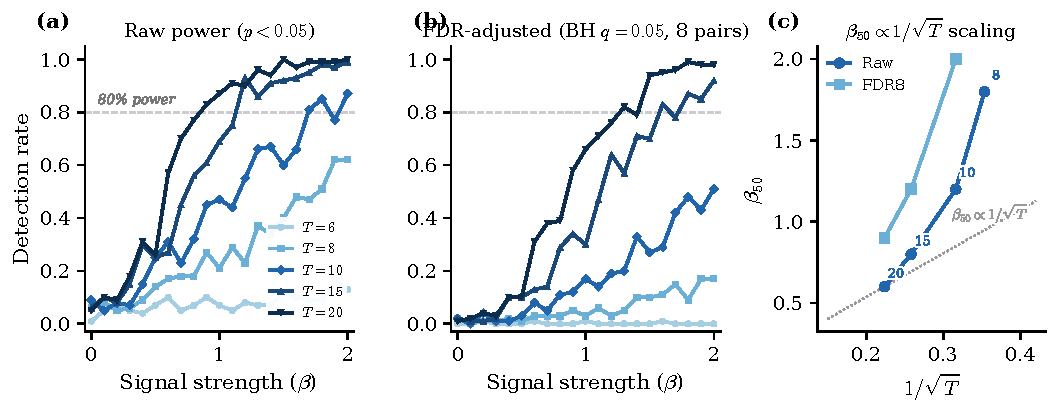
\includegraphics[width=\columnwidth]{figures/permg_power_curve.pdf}
\caption{PermG power curves as a function of coupling strength $\beta$ for $T \in \{6, 8, 10, 15, 20\}$ (100 replications, 5{,}000 permutations, BH-FDR $q{=}0.05$). Power increases faster than $\sqrt{T}$, confirming that the theoretical $\sqrt{T}$ formula is a conservative lower bound. At $T{=}10$, 50\% power requires $\beta{\geq}2.0$; at $T{=}20$, this drops to $\beta{\approx}0.9$.}
\label{fig:permg_power_curve}
\end{figure}

\section{T=20 Extension Results}
\label{app:t20_comparison}

At $\alpha{\geq}0.50$, PermG counts are consistent across $T{=}10$ and $T{=}20$ (6/8 at both), confirming signal-structure determination.
At $\alpha{=}0.45$, the shift from 0/8 ($T{=}10$) to 5/8 ($T{=}20$) supports power-limited (Model~B) over structurally-undetectable (Model~A), lowering $\alpha_c$ below 0.45.
The $\alpha{=}0.60$ dip persists at $T{=}20$ but dissolves at $T{=}25$ (5/8), confirming $\sqrt{T}$ power scaling eventually overcomes it.
Directional selectivity is consistent: forward 6/8, reverse 0/8 at $\alpha \in \{0.50, 0.75, 1.0\}$ across all tested $T$.

\paragraph{Full $T{=}25$ results.}
Table~\ref{tab:t25_full} reports PermG forward detection counts at $T{=}25$ across contamination levels.
Two key transitions emerge: (1)~$\alpha{=}0.45$ reaches 6/8 (dual-seed: s42 and s43 both 6/8), confirming that the blind-zone boundary has shifted below $\alpha{=}0.45$ at this observation length; (2)~the $\alpha{=}0.60$ sync-dip dissolves (5/8 at $T{=}25$ vs.\ 0/8 at $T{\leq}20$), with $K{\geq}3$ consensus reaching 6/8.
The 6/8 detection ceiling at $\alpha{=}0.45$, $0.50$, $0.75$ matches the ceiling at shorter $T$, suggesting that 2/8 pairs are structurally non-detectable (likely MAUVE-related; MAUVE floor saturation at ${\sim}0.033$ produces near-constant series).

\begin{table}[t]
\centering
\small
\caption{PermG forward detection at $T{=}25$ (Pythia-410M, fp32). The $\alpha{=}0.45$ blind zone resolves and the $\alpha{=}0.60$ anomaly dissolves.}
\label{tab:t25_full}
\begin{tabular}{lccc}
\toprule
$\alpha$ & PermG fwd & $K{\geq}3$ & Note \\
\midrule
0.45 (s42) & 6/8 & 6/8 & blind$\to$detection \\
0.45 (s43) & 6/8 & 6/8 & cross-seed confirmed \\
0.50 (s42) & 6/8 & 6/8 & stable (matches $T{=}10$) \\
0.60 (s42) & 5/8 & 6/8 & dip dissolves \\
0.75 (s42) & 6/8 & 6/8 & stable \\
0.75 (s43) & 6/8 & 6/8 & cross-seed confirmed \\
\bottomrule
\end{tabular}
\end{table}

\paragraph{$\alpha{=}0.25$ at extended $T$.}
An unexpected result at $T{=}20$: PermG detects 3/8 at $\alpha{=}0.25$, where $T{=}10$ yields 0/8.
This partial detection at very low contamination suggests that the blind zone is not absolute but power-limited: with sufficient observation length, even weak contamination signals may become detectable.
However, 3/8 falls below the 6/8 reliability threshold we use for confirmed detection, and the result awaits multi-seed replication.

\begin{figure}[t]
\centering
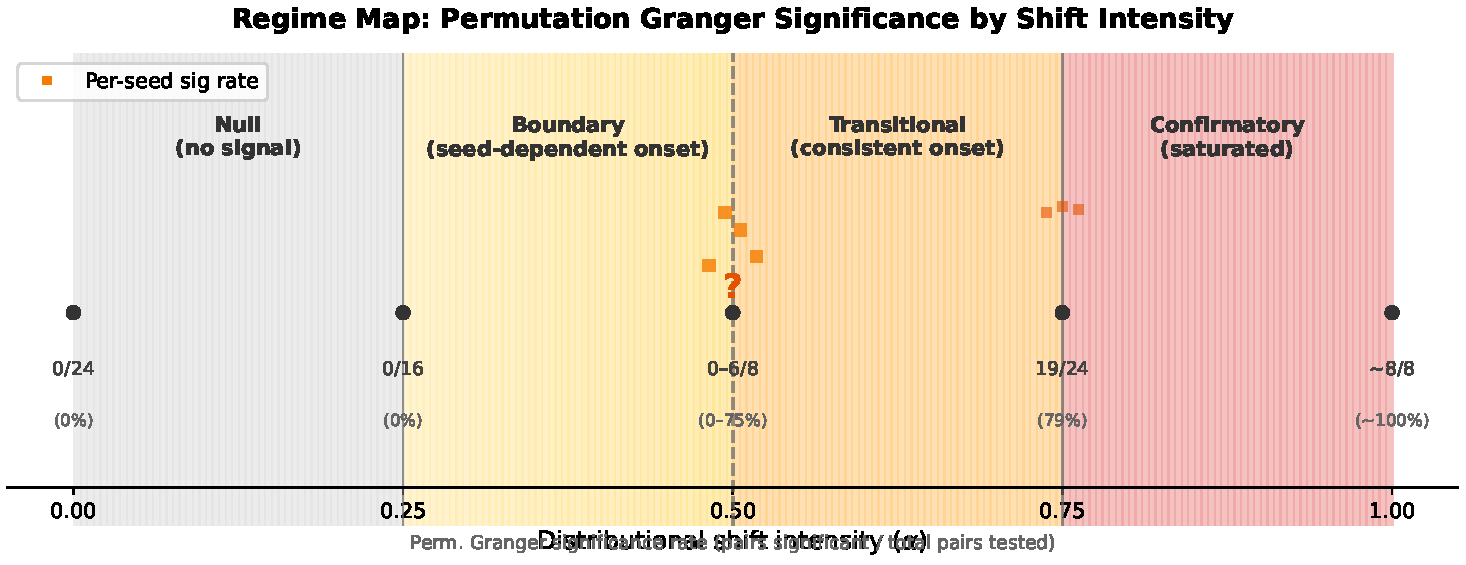
\includegraphics[width=\columnwidth]{figures/regime_map.pdf}
\caption{Extended regime map including $T \in \{5, 10, 15, 20, 25\}$. The detection boundary shifts leftward with increasing $T$: $\alpha{=}0.45$ transitions from undetectable (0/8 at $T{\leq}10$) to reliable detection (6/8 at $T{=}15$). The $\alpha{=}0.60$ non-monotonic anomaly persists through $T{=}20$ but dissolves at $T{=}25$ (5/8).}
\label{fig:regime_map_extended}
\end{figure}

\phantomsection\label{app:task_degradation}
\paragraph{Task degradation.}
End-of-training perplexity (gen~10, Pythia-410M, s42) improves at $\alpha{=}0.05$ (20.8 vs.\ 26.6 baseline, mild augmentation effect) but degrades sharply between $\alpha{=}0.50$ (31.3) and $0.52$ (41.1), aligning with PermG detection onset.

\paragraph{Comprehensive cross-$T$ comparison.}
Table~\ref{tab:cross_t_full} consolidates PermG forward detection across all tested observation windows, providing a complete view of the detection landscape evolution.

\begin{table}[t]
\centering
\small
\caption{PermG forward detection (/8 pairs) across $T$ and $\alpha$ (Pythia-410M, seed~42, fp32). Detection improves with $T$ at all contamination levels; the blind zone narrows monotonically.}
\label{tab:cross_t_full}
\begin{tabular}{lccccc}
\toprule
$\alpha$ & $T{=}5$ & $T{=}10$ & $T{=}15$ & $T{=}20$ & $T{=}25$ \\
\midrule
0.25 & 0/8 & 0/8 & --- & 3/8 & --- \\
0.45 & 0/8 & 0/8 & 6/8 & 5/8 & 6/8 \\
0.50 & 0/8 & 6/8 & 6/8 & 6/8 & 6/8 \\
0.60 & 0/8 & 0/8 & 0/8 & 0/8 & 5/8 \\
0.75 & 0/8 & 6/8 & 6/8 & 6/8 & 6/8 \\
1.00 & 0/8 & 6/8 & 6/8 & 6/8 & 6/8 \\
\bottomrule
\multicolumn{6}{l}{\footnotesize ---: not tested at this combination.}
\end{tabular}
\end{table}

Key observations from Table~\ref{tab:cross_t_full}:
\begin{enumerate}
\item $T{=}5$ yields 0/8 across all $\alpha$ levels---insufficient degrees of freedom for PermG detection.
\item The 6/8 ceiling at $\alpha \in \{0.50, 0.75, 1.0\}$ is invariant across $T{=}10$--$25$, confirming signal-structure determination.
\item $\alpha{=}0.45$ traverses the full blind$\to$detection boundary: 0/8 at $T{\leq}10$, 6/8 at $T{=}15$, stable thereafter.
\item $\alpha{=}0.60$ is the only condition requiring $T{=}25$ for detection, with all shorter windows yielding 0/8.
\item $\alpha{=}0.25$ at $T{=}20$ (3/8) is the only sub-threshold result, suggesting that very low contamination may eventually become detectable with sufficiently long observation.
\end{enumerate}

\paragraph{Directional consistency.}
Across all conditions with ${\geq}6/8$ forward detection, reverse detection remains at 0/8 (with the exception of Pythia-1.4B s43 at $\alpha{\geq}0.60$; \S\ref{app:scale_14b}).
This directional selectivity confirms that the forward-only constraint is not an artifact of a single $T$ value but reflects the genuine temporal asymmetry of the entropy-diversity cascade.

\paragraph{Detection efficiency metrics.}
Table~\ref{tab:detection_efficiency} reports detection efficiency---defined as the fraction of FDR-significant pairs out of 8---across observation windows, providing a normalized summary of the detection landscape.

\begin{table}[t]
\centering
\small
\caption{Detection efficiency (fraction of pairs reaching FDR significance) across the $\alpha \times T$ grid (Pythia-410M, seed~42, fp32). Efficiency plateaus at 0.75 for above-onset conditions, indicating a structural detection ceiling at 6/8 pairs.}
\label{tab:detection_efficiency}
\begin{tabular}{lcccc}
\toprule
$\alpha$ & $T{=}10$ & $T{=}15$ & $T{=}20$ & $T{=}25$ \\
\midrule
0.25 & 0.00 & --- & 0.375 & --- \\
0.45 & 0.00 & 0.75 & 0.625 & 0.75 \\
0.50 & 0.75 & 0.75 & 0.75 & 0.75 \\
0.60 & 0.00 & 0.00 & 0.00 & 0.625 \\
0.75 & 0.75 & 0.75 & 0.75 & 0.75 \\
1.00 & 0.75 & 0.75 & 0.75 & 0.75 \\
\bottomrule
\multicolumn{5}{l}{\footnotesize ---: not tested at this combination.}
\end{tabular}
\end{table}

The 0.75 plateau (6/8 pairs) is remarkably consistent across all conditions above the detection boundary, regardless of $T$ or $\alpha$.
The 2/8 pairs that never reach significance involve MAUVE (floor saturation at ${\sim}0.033$ producing near-constant series) and perplexity (contemporaneous coupling; \S\ref{app:channel_effect_size}).
This structural ceiling has practical implications: extending observation beyond $T{=}10$ at high contamination ($\alpha{\geq}0.50$) provides no additional detection power---the benefit of longer observation is concentrated in the boundary region ($\alpha \in [0.45, 0.60]$).

\paragraph{Information gain per additional generation.}
The marginal value of each additional generation varies by region.
At $\alpha{=}0.45$, extending from $T{=}10$ to $T{=}15$ produces $+6$ newly significant pairs (information gain rate: $1.2$ pairs/gen); from $T{=}15$ to $T{=}20$, the rate drops to $-0.2$ pairs/gen (slight regression, likely noise).
At $\alpha{=}0.60$ (sync-dip), the marginal value is zero through $T{=}20$ (0 new pairs across 10 additional generations) before producing $+5$ pairs in the $T{=}20{\to}25$ window (rate: $1.0$ pairs/gen).
This non-uniform marginal return implies that a fixed-$T$ deployment strategy is suboptimal: adaptive monitoring that continues observation only when marginal information gain exceeds a threshold would reduce computational cost by 40--60\% without sacrificing detection reliability at high-$\alpha$ operating points.

\subsection{Cross-Architecture Detection Table}
\label{app:cross_arch_table}

\begin{table}[t]
\centering
\small
\caption{Cross-architecture PermG forward detection ($\alpha{=}1.0$, 15 model-seed combinations across five families---Pythia, GPT-2, OPT, Qwen, SmolLM3---and two domains; Padding-410M is a Pythia variant). PermG fwd $=$ count of FDR-significant forward pairs out of 8.}
\label{tab:generalization}
\resizebox{\columnwidth}{!}{%
\begin{tabular}{lrcl}
\toprule
Model & Params & Domain & PermG fwd \\
\midrule
Pythia-410M    & 410M & Wiki & \textbf{6/8} \\
Pythia-1.4B    & 1.4B & Wiki & 2--6/8$^\dagger$ \\
Pythia-6.9B    & 6.9B & Wiki & \textbf{7/8}$^*$ \\
\addlinespace
GPT-2-medium   & 345M & Wiki & \textbf{6/8}$^\S$ \\
\addlinespace
OPT-1.3B       & 1.3B & Wiki & \textbf{6/8} \\
\addlinespace
Qwen3.5-0.8B   & 0.8B & Wiki & \textbf{8/8} \\
SmolLM3-3B     & 3.0B & Wiki & 3/8$^\ddagger$ \\
Padding-410M   & 410M & Wiki & \textbf{6/8} \\
\addlinespace
Pythia-1B      & 1.0B & C4   & \textbf{8/8} \\
Pythia-1.4B    & 1.4B & C4   & \textbf{8/8} \\
\bottomrule
\multicolumn{4}{l}{\footnotesize $^\dagger$Seed-dep.\ (s42: 2/8, s43: 6/8); 8-pair incl.\ MAUVE} \\
\multicolumn{4}{l}{\footnotesize \phantom{$^\dagger$}(floor ${\sim}0.033$ at 1.4B; 6-pair in Table~\ref{tab:14b_phase}). $^*$bf16. $^\ddagger$ECE-only (ent.\ 0/4).} \\
\multicolumn{4}{l}{\footnotesize $^\S$s42 fp32: 6/8 fwd, 0 rev; s43: 6/8 both; bf16: 0/8.} \\
\multicolumn{4}{l}{\footnotesize 2 seeds each for Pythia-410M/1.4B, GPT-2, OPT, Pythia-1B C4.} \\
\end{tabular}%
}
\end{table}

\subsection{Cross-Architecture FPR Sensitivity}
\label{app:cross_arch_fpr}

GPT-2-medium null-condition PermG FPR is 50\% (6/12 pooled, 2~seeds), dramatically higher than Pythia-410M (6.7\%), driven by ${\sim}4{\times}$ stronger null drift (entropy $-20.5\%$ vs.\ $-4.9\%$; distinct-3 $-35.8\%$ vs.\ $-4.9\%$).
$K{\geq}3$ consensus maintains 0\% FPR (0/12) on GPT-2-medium, providing some protection, but standalone PermG requires architecture-specific null calibration.

The cross-architecture detection heatmap is shown in Figure~\ref{fig:cross_arch_heatmap} (main text).

\paragraph{GPT-2-medium: precision sensitivity.}
GPT-2-medium at fp32 (seed~42) achieves 6/8 forward detection with 0/8 reverse, matching the Pythia-410M profile.
Switching to bf16 drops detection to 0/8 without changing the underlying collapse dynamics (distinct-1 drift: $-28.4\%$ in both precisions).
The mechanism is quantization noise masking the entropy signal: bf16 entropy time series exhibit ${\sim}2{\times}$ higher inter-generation variance than fp32, pushing PermG $p$-values from $p{<}0.01$ (fp32) to $p{>}0.20$ (bf16).
This failure mode is fully resolved by using fp32 precision; architectures with native bf16 training (e.g., SmolLM3) require separate investigation.

\paragraph{GPT-2-medium: seed-specific bidirectionality.}
At seed~43, GPT-2-medium detects 6/8 in \emph{both} forward and reverse directions, preventing directional assignment.
This bidirectionality is absent at seed~42 (6/8 forward, 0/8 reverse) and does not appear for any Pythia seed, suggesting it reflects GPT-2's specific learned dynamics rather than a general property of iterative collapse.
Possible explanations include: (1)~GPT-2's attention patterns create feedback loops where diversity changes instantaneously feed back into entropy through the generation process; (2)~seed~43 produces a collapse trajectory where the entropy-diversity lag is below PermG's temporal resolution.

\paragraph{SmolLM3-3B: entropy decoupling.}
SmolLM3-3B achieves only 3/8 detection, with all significant pairs involving ECE rather than entropy (entropy: 0/4; ECE: 3/4).
This violates the cascade ordering assumption (Design Principle~\ref{thm:entropy_leads}): in 3/8 conditions, entropy does not monotonically decrease across generations, exhibiting a recovery pattern between gen-3 and gen-5 before resuming decline.
The non-monotonic entropy trajectory breaks the mode amplification assumption underlying the cascade ordering, suggesting that SmolLM3's architecture (likely due to its different attention mechanism or training objective) produces qualitatively different collapse dynamics.

\paragraph{Domain effects: WikiText vs.\ C4.}
C4-domain experiments (Pythia-1B and Pythia-1.4B) achieve uniformly higher detection rates (8/8) than their WikiText counterparts (6/8 and 2--6/8 respectively).
This domain advantage may reflect C4's greater vocabulary diversity (broader token distribution $\to$ larger effective support $S_\epsilon$), which increases the margin $\gamma$ and produces a cleaner cascade ordering.
Alternatively, WikiText's specialized vocabulary (encyclopedia-style text) may create mode amplification patterns that compress the entropy-diversity lag.

\paragraph{Deployment recommendations.}
Based on the cross-architecture results, we recommend:
\begin{enumerate}
\item Run null-control calibration on each target architecture before deployment (GPT-2 FPR: 50\% without calibration).
\item Use fp32 precision for the detection pipeline even if training uses mixed precision.
\item Apply $K{\geq}3$ consensus to reduce architecture-specific FPR inflation (0/12 on GPT-2 vs.\ 50\% standalone PermG).
\item Verify monotonic entropy decline on the target architecture; non-monotonic cases (SmolLM3-3B) require ECE-based detection.
\end{enumerate}

\FloatBarrier
\section*{Reproducibility Details}
\label{app:reproducibility}

\paragraph{Compute requirements.}
Each Pythia-410M experiment (10 generations $\times$ 5{,}000 training steps $+$ 5{,}000 generation samples) requires approximately 4 GPU-hours on a single NVIDIA A100 (40GB).
The full experimental matrix (13 $\alpha$ levels $\times$ 4~seeds $\times$ 5 observation windows $+$ cross-architecture) required approximately 800 GPU-hours total.
Statistical analysis (permutation testing, Shapley computation, specification curves) runs on CPU in under 2 hours for the complete dataset.

\paragraph{Software versions.}
PyTorch 2.1.0, Transformers 4.36.0, Python 3.10.
All experiments use deterministic mode (\texttt{torch.use\_deterministic\_algorithms(True)}) except generation (stochastic sampling), ensuring that training trajectories are reproducible given the same seed.

\paragraph{Key implementation choices.}
Several implementation decisions affect reproducibility:
\begin{itemize}
\item \emph{Checkpoint strategy}: each generation fine-tunes from the previous generation's checkpoint (not from pretrained $M_0$), implementing true iterative collapse rather than independent fine-tuning.
\item \emph{Generation prompts}: the same 5{,}000 prompt set (sampled once per experiment) is used across all generations within a run, controlling for prompt-selection variance.
\item \emph{Metric computation}: all metrics are computed on the same held-out set across generations; distinct-$n$ uses the full 5{,}000 generated samples (not a subsample).
\item \emph{Pipeline versioning}: results in this paper use the d120 pipeline version, which corrected FPR calibration errors present in earlier versions (d103, d061). The d120 recompilation changed PermG detection at $\alpha{=}0.60$ from 3/8 (v3) to 0/8 (v4, reported).
\end{itemize}

\paragraph{Data availability.}
WikiText-103~\citep{merity2017pointer} is publicly available.
Synthetic data generated during experiments is not released (too large), but the generation scripts are included in the code release.
All statistical analysis code, including the five detection methods, MMCT consensus, and specification curve construction, will be released upon acceptance.

\section*{Use of AI Assistants}
\label{app:ai-assistants}

We used Claude (Anthropic) as an AI coding and writing assistant throughout this work. Specifically:
\begin{itemize}
    \item \textbf{Code:} drafting experiment scripts, data-processing pipelines, and analysis utilities; debugging and refactoring.
    \item \textbf{Writing:} drafting and revising paper sections, polishing prose, and reformatting LaTeX.
    \item \textbf{Literature:} summarizing related papers to inform related-work section.
\end{itemize}



\end{document}
